\documentclass[10pt]{memoir}
\setstocksize{220mm}{155mm} 	        
\settrimmedsize{220mm}{155mm}{*}	
\settypeblocksize{170mm}{116mm}{*}	
\setlrmargins{18mm}{*}{*}
\setulmargins{*}{*}{1.2}
%\setlength{\headheight}{5pt}%
\checkandfixthelayout[lines]
\linespread{1.16}
\flushbottom

%%% Hyphenation settings
\usepackage[htt]{hyphenat}
\hyphenation{he-lio-trope opos-sum}
\tracingparagraphs=1
%Hyphenation in Devanāgarī of the edition still missing? Probably this needs to be modified in babel-iast package? 

%%% babel
\usepackage[english]{babel}
\usepackage{babel-iast/babel-iast}

\babelfont[iast]{rm}[Renderer=Harfbuzz, Scale=1.3]{AdishilaSan}%AdishilaSan}
\babelfont[english]{rm}{Adobe Text Pro}

%%% more functionality
\PassOptionsToPackage{hyphens}{url}
\usepackage{hyperref}
\usepackage{pdflscape}
\usepackage{cleveref}
\usepackage{url}
\usepackage{cleveref}
\usepackage{microtype}
\usepackage{lineno}

%\usepackage{bigfoot}
%%% more functions
\usepackage[dvipsnames]{xcolor}
%\usepackage[para,perpage]{footmisc}

%%%für den Counter von Kapiteln und Sätzen! 
\newcommand{\uproman}[1]{\uppercase\expandafter{\romannumeral#1}}
\newcommand{\lowroman}[1]{\romannumeral#1\relax}

\makeindex
\newfontfamily\sanskritfont[Script=Devanagari,Mapping=RomDev,Scale=1.1]{Sanskrit2003}
\usepackage{pifont,fourier-orns,lettrine,psvectorian,paralist,enumitem,pdfpages,wrapfig,tabulary,lettrine,longtable}
\setlist[enumerate]{itemsep=0mm}
\usepackage[autostyle]{csquotes}
\usepackage[defaultlines=2,all]{nowidow}
\usepackage{ellipsis,adforn,booktabs,longtable,url,tikz}
\lineskiplimit=-3pt          

\makechapterstyle{IeT}{%
  \chapterstyle{default}
  \renewcommand*{\printchapternonum}{\centering}
  \renewcommand*{\clearforchapter}{\cleartorecto} 
  \aliaspagestyle{chapter}{empty}}
\chapterstyle{IeT}
\setsecnumdepth{none}  \openright  \nouppercaseheads
\settocdepth{subsubsection}

%%%% test better pagebreaks
%\def\fussy{%
%  \emergencystretch\z@
%  \tolerance 200%
%  \hfuzz .1\p@
%  \vfuzz\hfuzz}

%\interfootnotelinepenalty=10000\relax

%\usepackage[maxfloats=256]{morefloats}

%\maxdeadcycles=500

%raggedbottomsectiontrue
%%\checkandfixthelayout


%%%%%%%  biblatex
%\newcommand{\noun}[1]{\textsc{#1}}    %  philosophy-verbose
\usepackage[backend=biber, sorting=nyt, style=verbose]{biblatex} %%%%ORIGINAL TiE
\renewcommand*{\mkbibnamefamily}[1]{\textsc{#1}}


\DeclareFieldFormat{url}{%
  \mkbibacro{URL}\addcolon\space
  \href{#1}{\nolinkurl{\thefield{urlraw}}}}

\DeclareFieldFormat{citeurl}{%
  \href{#1}{\nolinkurl{\thefield{urlraw}}}} 


\DeclareFieldFormat{postnote}{#1}
\renewcommand{\postnotedelim}{, }
\addbibresource{bindu.bib}

%%% ekdosis
\usepackage[teiexport=tidy,parnotes=true]{ekdosis}% =tidy cleans up HTML and XML documents by fixing markup errors and upgrading legacy code to modern standards. parnotes=footnotes below or above critical apparatus

\SetLineation{lineation=page, modulo} %lineation=page sets thenumbering to start afresh at the top of each page. =modulo makes every fifth line numbered. {lineation=page} makes every line numbered! 

\renewcommand{\linenumberfont}{\selectlanguage{english}\footnotesize} %sets language of lines to English

\SetTEIxmlExport{autopar=false} %autopar=falseinstructs ekdosis to ignore blank lines in the.tex sourcefile as markers for paragraph boundaries. As a result, each paragraph of the edition must be found within an environment associated with the xml <p> element

\SetHooks{
  lemmastyle=\bfseries,
  %refnumstyle=\selectlanguage{english}\bfseries,
  refnumstyle=\selectlanguage{english}\color{blue}\bfseries,
  appheight=0.8\textheight,
}

\newif\ifinapparatus
\DeclareApparatus{source}[
%bhook=\inapparatustrue,
lang=english,
notelang=english,
% bhook=\selectlanguage{english},
bhook=\selectlanguage{english}\textbf{Sources:},%
%maxentries=4, 
%ehook=.]
%sep={] },
%nosep,
]

\newif\ifinapparatus
\DeclareApparatus{testium}[
%bhook=\inapparatustrue,
lang=english,
notelang=english,
% bhook=\selectlanguage{english},
bhook=\selectlanguage{english}\textbf{Testimonia:},
%maxentries=4, 
%ehook=.]
%nosep, 
]

% Declare \ifinapparatus and set \inapparatustrue at the beginning of
% the apparatus criticus block. Also set the language.  
\newif\ifinapparatus
  \DeclareApparatus{default}[
  %bhook=\inapparatustrue, 
  lang=english,
  %maxentries=33,
  %bhook=\selectlanguage{english},
  sep = {] },
  delim=\hskip 0.75em,
  rule=\rule{0.7in}{0.4pt},
]

\newif\ifinapparatus
\DeclareApparatus{philcomm}[
%bhook=\inapparatustrue,
lang=english,
notelang=english,
bhook=\selectlanguage{english}\textbf{Philological Commentary:},
%bhook=\selectlanguage{english},
sep={: },
]

\ekdsetup{
showpagebreaks,
spbmk = \textcolor{blue}{spb},
hpbmk = \textcolor{red}{hpb}
}

%\usepackage{fnpos}
%\makeFNmid
%\makeFNbottom
\usepackage[bottom]{footmisc}
%%%%%%%%%%%%%%%%%%%%%%%%%%%
\makeatletter
\def\blfootnote{\gdef\@thefnmark{}\@footnotetext}
\makeatother
%%%%%%%%%%%%%%%%%%%%%%%%%


% Macros and Definitions for the Print of Sigla
\def\acpc#1#2#3{{#1}\rlap{\textrm{\textsuperscript{#3}}}\textsubscript{\textrm{#2}}\space}
\def\sigl#1#2{{{#1}}\textsubscript{\textrm{#2}}}
\def\None{{\sigl{N}{1}}} \def\Noneac{\acpc{N}{1}{ac}\,} \def\Nonepc{\acpc{N}{1}{pc}\,}
\def\Ntwo{{\sigl{N}{2}}} \def\Noneac{\acpc{N}{2}{ac}\,} \def\Nonepc{\acpc{N}{2}{pc}\,}
\def\Done{{\sigl{D}{1}}} \def\Doneac{\acpc{D}{1}{ac}\,} \def\Donepc{\acpc{D}{1}{pc}\,}
\def\Dtwo{{\sigl{D}{2}}} \def\Dtwoac{\acpc{D}{2}{ac}\,} \def\Dtwopc{\acpc{D}{2}{pc}\,}
\def\Uone{{\sigl{U}{1}}} \def\Uoneac{\acpc{U}{1}{ac}\,} \def\Uonepc{\acpc{U}{1}{pc}\,}                 
\def\Utwo{{\sigl{U}{2}}} \def\Utwoac{\acpc{U}{2}{ac}\,} \def\Utwopc{\acpc{U}{2}{pc}\,}

%%%%%%%%%%%%%% Tattvabinduyoga - List of Witnesses   %%%%%%%%%%%%%%%%%%%
\DeclareWitness{ceteri}{\selectlanguage{english}cett.}{ceteri}[]   
\DeclareWitness{E}{\selectlanguage{english}E}{Printed Edition}[]    
\DeclareWitness{P}{\selectlanguage{english}P}{Pune BORI 664}[]  
\DeclareWitness{B}{\selectlanguage{english}B}{Bodleian 485}[]       
\DeclareWitness{N1}{\selectlanguage{english}N\textsubscript{1}}{NGMPP 38/31}[]
\DeclareWitness{N2}{\selectlanguage{english}N\textsubscript{2}}{NGMPP B 38/35}[]
\DeclareWitness{L}{\selectlanguage{english}L}{LALCHAND 5876}[]  
\DeclareWitness{D}{\selectlanguage{english}D}{IGNCA 30019}[] 
%\DeclareWitness{D2}{\selectlanguage{english}D\textsubscript{2}}{IGNCA 30020}[]  
\DeclareWitness{U1}{\selectlanguage{english}U\textsubscript{1}}{SORI 1574}[] 
\DeclareWitness{U2}{\selectlanguage{english}U\textsubscript{2}}{SORI 6082}[]
%%%%%%%%%%%%%% Tattvabinduyoga - Groups of Witnesses   %%%%%%%%%%%%%%%%%%%
\DeclareWitness{X}{\selectlanguage{english}\alpha}{Alpha Group: D,N1,N2,U1}[]
\DeclareWitness{Y}{\selectlanguage{english}\beta}{Beta Group: B,E,L,P,U2}[]
%%%%%%%%%%%%% Testimonia
\DeclareWitness{Ysv}{\selectlanguage{english}Ysv}{Yogasvarodaya}[] %%%add infos!  

%%%%%%%%%%%%%%%%%%%%%%%%%%%%%%%%%%%%%%%%%%%
% Macro for Editing Abbrevs.
\def\om{\textrm{\footnotesize \textit{om.}\ }} %prints om. for omitted in apparatus
\def\korr{\textrm{\footnotesize \textit{em.}\ }} %prints em. for emended in apparatus
\def\conj{\textrm{\footnotesize \textit{conj.}\ }} %prints conj. for conjectured in apparatus

% \supplied{text} EDITORIAL ADDITION -> Within \lem oder \rdg
% \surplus{text} EDITORIAL DELETION -> Within \lem oder \rdg
% \sic{text} CRUX
% \gap{text} LACUNAE -> [reason=??, unit=??, quantity=??, extent=??]


%%%%%%%%%%%%%%%%%%%%%%%%%%%%%%%%%%%%%%%%%%% All macros of this list can be used in 
% Macro for Editing Abbrevs.
\def\eyeskip{\textrm{{ab.\,oc. }}}
\def\aberratio{\textrm{{ab.\,oc. }}}
\def\ad{\textrm{{ad}}}
\def\add{\textrm{{add.\ }}}
\def\ann{\textrm{{ann.\ }}}
\def\ante{\textrm{{ante }}} 
\def\post{\textrm{{post }}}
%\def\ceteri{cett.\,}                   
\def\codd{\textrm{{codd.\ }}}

\def\coni{\textrm{{coni.\ }}}
\def\contin{\textrm{{contin.\ }}}
\def\corr{\textrm{{corr.\ }}}
\def\del{\textrm{{del.\ }}}
\def\dub{\textrm{{ dub.\ }}}

\def\expl{\textrm{{explic.\ }}} 
\def\explica t{\textrm{{explic.\ }}}
\def\fol{\textrm{{fol.\ }}}
\def\foll{\textrm{{foll.\ }}}
\def\gloss{\textrm{{glossa ad }}}
\def\ins{\textrm{{ins.\ }}}      
\def\inseruit{\textrm{{ins.\ }}} 
\def\im{{\kern-.7pt\lower-1ex\hbox{\textrm{\tiny{\emph{i.m.}}}\kern0pt}}} %\textrm{\scriptsize{i.m.\ }}}      
\def\inmargine{{\kern-.7pt\lower-.7ex\hbox{\textrm{\tiny{\emph{i.m.}}}\kern0pt}}}%\textrm{\scriptsize{i.m.\ }}}      
\def\intextu{{\kern-.7pt\lower-.95ex\hbox{\textrm{\tiny{\emph{i.t.}}}\kern0pt}}}%\textrm{\scriptsize{i.t.\ }}}           
\def\indist{\textrm{{indis.\ }}}  
\def\indis{\textrm{{indis.\ }}}
\def\iteravit{\textrm{{iter.\ }}} 
\def\iter{\textrm{{iter.\ }}}
\def\lectio{\textrm{{lect.\ }}}   
\def\lec{\textrm{{lect.\ }}}
\def\leginequit{\textrm{{l.n. }}} 
\def\legn{\textrm{{l.n. }}}
\def\illeg{\textrm{{l.n. }}}

\def\primman{\textrm{{pr.m.}}}
\def\prob{\textrm{{prob.}}}
\def\rep{\textrm{{repetitio }}}
\def\secundamanu{\textrm{\scriptsize{s.m.}}}            \def\secm{{\kern-.6pt\lower-.91ex\hbox{\textrm{\tiny{\emph{s.m.}}}\kern0pt}}}%   \textrm{\scriptsize{s.m.}}}
\def\sequentia{\textrm{{seq.\,inv.\ }}}  
\def\seqinv{\textrm{{seq.\,inv.\ }}}
\def\order{\textrm{{seq.\,inv.\ }}}
\def\supralineam{{\kern-.7pt\lower-.91ex\hbox{\textrm{\tiny{\emph{s.l.}}}\kern0pt}}} %\textrm{\scriptsize{s.l.}}}
\def\interlineam{{\kern-.7pt\lower-.91ex\hbox{\textrm{\tiny{\emph{s.l.}}}\kern0pt}}}   %\textrm{\scriptsize{s.l.}}}
\def\vl{\textrm{v.l.}}   \def\varlec{\textrm{v.l.}} \def\varialectio{\textrm{v.l.}}
\def\vide{\textrm{{cf.\ }}}
\def\cf{\textrm{{cf.\ }}} 
\def\videtur{\textrm{{vid.\,ut}}}
\def\crux{\textup{[\ldots]} }
\def\cruxx{\textup{[\ldots]}}
\def\unm{\textit{unm.}}
%%%%%%%%%%%%%%%%%%%%%%%%%%%%%%%%%%%%

% List of Scholars
\DeclareScholar{ego}{ego}[
forename=Nils Jacob,
surname=Liersch]

% Persons:14\DeclareScholar{ego}{ego}[15forename=Robert,16surname=Alessi]17% Useful shorthands:18\DeclareShorthand{codd}{codd.}{V,I,R,H}19\DeclareShorthand{edd}{edd.}{Lit,Erm,Sm}20\DeclareShorthand{egoscr}{\emph{scripsi}}{ego}

%Useful shorthands:
%\DeclareShorthand{codd}{codd.}{V,I,R,H}
%\DeclareShorthand{edd}{edd.}{Lit,Erm,Sm}
\DeclareShorthand{egoscr}{em.}{ego}
\DeclareShorthand{egoscrconj}{conj.}{ego}
\DeclareShorthand{egomute}{\unskip}{ego}

\usepackage{xparse}

\NewDocumentEnvironment{tlg}{O{}O{}}{\setlength{\leftskip}{0pt}\vspace{-1ex}\begin{quotation}}{\hfill #1\ \vspace{-1ex}\end{quotation}\vspace{-1ex}} %verse environment
%\NewDocumentEnvironment{tlg}{O{}O{}}{\begin{verse}}{॥#1\hskip-4pt ॥\\ \end{verse}}
\NewDocumentCommand{\tl}{m}{{\selectlanguage{iast} #1}}

\NewDocumentCommand{\extra}{m}{{\textcolor{gray}{#1}}} %command for additions to U2
\NewDocumentCommand{\crazy}{m}{{\textcolor{red}{#1}}} %totally corrupted passage
\NewDocumentCommand{\coro}{m}{{\textcolor{violet}{#1}}} %colour for sentence counter! 

\NewDocumentEnvironment{prose}{O{}}{\begin{otherlanguage}{iast}}{\end{otherlanguage}}
% \NewDocumentEnvironment{padd}{O{}}{\begin{otherlanguage}{iast}}{\end{otherlanguage}}
\NewDocumentEnvironment{tlate}{O{}}
%\NewDocumentEnvironment{tadd}{O{}}

%Define two commands: \skp ("sanskrit plus"), to be ignored by TeX in
%the edition text, but processed in the TEI output. Conversely, \skm
%("sanskrit minus") is to be processed in the edition text, but
%ignored if found in the apparatus criticus and in the TEI output:

\NewDocumentCommand{\skp}{m}{}
\TeXtoTEIPat{\skp {#1}}{#1}

%\NewDocumentCommand{\skpp}{m}{}
%\TeXtoTEIPat{\skpp {#1}}{#1}

\NewDocumentCommand{\skm}{m}{\unless\ifinapparatus#1-\fi}
\TeXtoTEIPat{\skm {#1}}{}

% \NewDocumentCommand{\dd}{}{/\hskip-4pt/}
\NewDocumentCommand{\dd}{}{\mbox{/\hskip-4pt/}}
\TeXtoTEIPat{\dd {}}{//}


%%% modify environments and commands
%%% TEI mapping
\TeXtoTEIPat{\begin {tlg}}{<lg>} %lg=(Group of verse (s)) contains one or more verses or lines of verse that together form a formal unit (e.g. stanza, chorus).
\TeXtoTEIPat{\end {tlg}}{</lg>}

\TeXtoTEIPat{\begin {prose}}{<p>}
\TeXtoTEIPat{\end {prose}}{</p>}

\TeXtoTEIPat{\begin {tlate}}{<p>}
\TeXtoTEIPat{\end {tlate}}{</p>}

\TeXtoTEIPat{\\}{}
\TeXtoTEIPat{\linebreak}{<br/>}
\TeXtoTEIPat{\noindent}{}
%\TeXtoTEI{tl}{l}
\TeXtoTEI{emph}{hi}
\TeXtoTEI{bigskip}{}
\TeXtoTEI{None}{N1}
\TeXtoTEI{Ntwo}{N2}
\TeXtoTEI{Done}{D1}
\TeXtoTEI{Dtwo}{D2}
\TeXtoTEI{Uone}{U1}
\TeXtoTEI{Utwo}{U2}
%\TeXtoTEIPat{/}{ |}
%\TeXtoTEI{//}{ ||}
\TeXtoTEIPat{\korr}{em. }
\TeXtoTEIPat{\conj}{conj.}
\TeXtoTEIPat{\om}{om.}
\TeXtoTEIPat{english}{}
\TeXtoTEIPat{\hskip}{}
\TeXtoTEIPat{\hskip-4pt}{}
\TeXtoTEIPat{\hskip-2pt}{}
\TeXtoTEIPat{-}{ }
\TeXtoTEIPat{4pt}{}
\TeXtoTEIPat{2pt}{}
\TeXtoTEIPat{\textcolor {#1}{#2}}{<hi rend="#1">#2</hi>} 

% Nullify \selectlanguage in TEI as it has been used in
% \DeclareWitness but should be ignored in TEI.
\TeXtoTEI{selectlanguage}{}



\FormatDiv{1}{\begin{center}\Large}{\end{center}}
\FormatDiv{2}{\begin{center}\small}{\end{center}}
\FormatDiv{3}{\bfseries}{.}
\title{Yogatattvabindu of Rāmacandra\\ A Critical Edition and Annotated Translation}
\date{\today}

\parindent=15pt
\begin{document}

% Zitiermöglichkeiten:
%\footcite[See][p.\,1]{goldstein01:_tibet_englis_diction_moder_tibet}
%\footnote{\cite{goldstein01:_tibet_englis_diction_moder_tibet}.}

\frontmatter
\thispagestyle{empty}
\begin{center}
  {\Large \emph{The Yogatattvabindu}}\\[3mm]
\end{center}



\newpage

\

\thispagestyle{empty}



\normalsize


\newpage


\begin{center}
\thispagestyle{empty}

\

\vskip 2mm

\begin{otherlanguage}{iast}
\LARGE \sanskritfont{Yogatattvabindu}
\end{otherlanguage}

\vskip .4cm

\Huge Yogatattvabindu \\[7mm]
\Large Critical Edition\\
with annotated Translation


\large

\vspace{3cm}

Von

Nils Jacob Liersch
\small
\vfill

\vfill

Indica et Tibetica Verlag \\ % $\cdot$ 
Marburg 2024

\vskip 6mm

\end{center}

\newpage
\newpage \ \thispagestyle{empty}
\small  \

\noindent

\
\vfill


\small
\noindent \textbf{Bibliographische Information Der Deutschen Bibliothek}

\noindent
Die Deutsche Bibliothek verzeichnet diese Publikation in der Deutschen Nationalbibliographie;
detaillierte bibliographische Informationen sind im Internet über http://dnb.ddb.de abrufbar.

\noindent
\textbf{Bibliographic information published by Die Deutschen Bibliothek}

\noindent
Die Deutsche Bibliothek lists this publication in the Deutsche Nationalbibliographie; detailed
bibliographic data is available in the Internet at http://dnb.ddb.de.  


\vskip 1cm

\noindent
\copyright\ Indica et Tibetica Verlag, Marburg 2024

\medskip

\noindent
Alle Rechte vorbehalten / All rights reserved

\medskip

\noindent
Ohne ausdrückliche Genehmigung des Verlages ist es nicht gestattet, das Werk oder einzelne Teile
daraus nachzudrucken, zu vervielfältigen oder auf Datenträger zu speichern.

\smallskip

\noindent
Apart from any fair dealing for the purpose of private study, research, criticism or review, no
part of this book may be reproduced or translated in any form, by print, photo form, microfilm, or
any other means without written permission. Enquiries should be made to the publishers.

\bigskip

\noindent
Satz: \ \ Nils Jacob Liersch \\
Herstellung: \ \ BoD – Books on Demand GmbH, Norderstedt  \\

\bigskip

\noindent
%\ISBN     

\normalsize

\newpage

%\maketitle
\clearpage
\tableofcontents
\addtocounter{page}{-1}
\thispagestyle{empty}
\clearpage


\mainmatter

\chapter{Conventions in the Critical Apparatus}
\section{Sigla in the Critical Apparatus}

\begin{itemize}
\item E : Printed Edition
\item P : Pune BORI 664
\item L : Lalchand Research Library LRL5876
\item B : Bodleian Oxford D 4587
\item \None : NGMPP B 38-31
\item \Ntwo : NGMPP B 38-35 / A 1327-14
\item \Done : IGNCA 30019
\item \Uone : SORI 1574
\item \Utwo: SORI 6082
\end{itemize}

\chapter{Critical Edition \& Annotated Translation}
\cleardoublepage
\begin{alignment}[
  texts=edition[class="edition"];
  translation[class="translation"],
  ]
  \begin{edition}
    \ekddiv{
      head={[\uproman{1}. \textbf{rājayogaprakāra}]},
      type=section,
      depth=2,
      n=I
    }
    \xmlhead[h01]{[I. rājayogaprakāra]}
\label{intro}
\begin{prose}[p01_01]
\noindent
%--------------------------
% śrīgaṇeśāya namaḥ /                                                     rājayogāntargataḥ //  binduyogaḥ   \E 
% śrīgaṇeśāya namaḥ /                                                     atha tattvabiṃduyogaprāraṃbhaḥ     \L
% śrīṇe ya maḥ /                                                          atha rājayoga         liṣyate      \P
% \om                                                                                                         \B      
% śrīgaṇeśāya namaḥ // śrī gurave namaḥ //                                atha rājayogaprakāro  likhyate //  \N1
% śrīgaṇeśāya namaḥ //                                                //  atha rājayogaprakāro  likhyate //  \N2
% śrīgaṇeśāya namaḥ // śrī sarasvatyai namaḥ // śrī nirañjanāya namaḥ //  atha rājayogaprakāro  likhyate //  \D
% śrīgaṇeśāya namaḥ /  oṃ śrī niraṃjanāya //                              atha rājayogaprakāra  likhyate //  \U1
% śrīgaṇeśāya namaḥ /                                                     atha rājayoga         likhyate //  \U2
%--------------------------
%Homage to Śrī Gaṇeśa. Now, the way of Rājayoga is laid down.
%--------------------------          
\note[type=source, labelb=_11b,labele=_11e, nosep]{cf. YSv (PT p. 831): atha rājayogaḥ || yogasvarodaye | īśvara uvāca | rājayogaṃ pravakṣyāmi śṛṇu sarvatra siddhidam | guhyādguhyataraṃ devi nānādharmaṃ parāt param rājayogena deveśi nṛpapūjyo bhaven naraḥ | rājayogī cirāyuś ca aṣṭaiśvaryamayo bhavet ||}
\app{\lem[wit={ceteri}]{śrīgaṇeśāya namaḥ}
        \rdg[wit={P}]{śrīṇeyamaḥ}
        \rdg[wit={N1}]{śrīgaṇeśāya namaḥ || śrīgurave namaḥ ||}
        \rdg[wit={D}]{śrīgaṇeśāya namaḥ || śrīsarasvatyai namaḥ || śrīnirañjanāya namaḥ ||}
        \rdg[wit={U1}]{śrīgaṇeśāya namaḥ || oṃ śrīniraṃjanāya ||}}\dd{}
\app{\lem[wit={D,N1,N2}]{atha rājayogaprakāro likhyate}
        \rdg[wit={U1}]{atha rājayogaprakāra likhyate}
        \rdg[wit={E}]{rājayogāntargataḥ || binduyogaḥ}
        \rdg[wit={L}]{atha tattvabiṃduyogaprāraṃbhaḥ}
        \rdg[wit={P}]{atha rājayoga liṣyate}
        \rdg[wit={U2}]{atha rājayoga likhyate}}/ 
%-------------------------- 
% \om                        \E
% \om                        \L
% \om                        \B
% rājayogasyedaṃ phalaṃ      \P
% rājayogasya idaṃ phalaṃ    \N1
% rājayogasya idaṃ phalaṃ    \N2
% rājayogasya idaṃ phalaṃ // \D
% rājayogasya idaṃ phalaṃ    \U1
% rājayogasyedaṃ phalaṃ /    \U2
%--------------------------    
\app{\lem[wit={P,U2}]{rājayogasyedaṃ phalaṃ}
  \rdg[wit={D,N1,N2}]{rājayogasya idaṃ phalaṃ}
  \rdg[wit={E,L}]{\om}}
%--------------------------
%This is the result of \textit{rājayoga}:
%--------------------------
% \om                                                                                                                                                                         \E
% \om                                                                                                                                                                         \L
% \om                                                                                                                                                                         \B
% yena rājayogenāneka---rājyabhogasamaya   eva   anekapārthivavinodaprekṣaṇasamaya  eva   bahutarakālaṃ  śarīrasthitir  bhavati    sa eva  rājayogaḥ tasyaite     bhedāḥ      \P
% yena rājayogenāneka---rājyabhogasamaya   eva/  anekapārthivavinodaprekṣaṇasamaya  eva/  bahutarakālaṃ  śarīrasthitir  bhavati    sa eva  rājayogaḥ /  tasya ete bhedāḥ /    \N1
% yena rājayogena  anekarājyabhogasamaya   eva// anekapārthivavinodaprekṣaṇasamaya  eva   bahuttarakālaṃ śarīrasthitir  bhavati    sa eva  rājayogaḥ /  tasya ete bhedāḥ /    \N2
% yena rājayogena  anekarājyabhogasamaya   eva// anekapārthivavinodaprekṣaṇasamaya  eva// bahutarakālaṃ  śarīrasthitir  bhavati//  sa eva  rājayogaḥ // tasya ete bhedāḥ /    \D
% yena rājayogena  anekarājyabhogasamaya   eva// anekapārthivavinodaprekṣaṇasamaya  eva// bahutarakālaṃ  śarīrasthitir  bhavati    sa evaṃ rājayogaḥ    tasya ete bhedāḥ //   \U1 
% yena rājayogena  anekarājyabhogasamaya   eva// anekapārthivavinodaprekṣyaṇasamaya eva// bahutarakālaṃ  śarīrasthitir  bhavati//  sa eva  rājayogastaisyaite     bhedāḥ //   \U2
% --------------------------
%\textit{Rājayoga} is that by which longterm durability of the body arises even amongst manifold royal pleasures even amongst the manifold royal entertainments and spectacle. This truly is \textit{rājayoga}. Of this [\textit{rājayoga}] these are the varieties: \end{tlate}
%--------------------------
yena rāja\app{\lem[wit={P,N1}, alt={°yogenāneka°}]{yogenāneka}
  \rdg[wit={D,N2,U1,U2}]{°yogena aneka°}
}rājyabhogasamaya eva anekapārthivavinoda\app{\lem[wit={ceteri}, alt={°prekṣaṇasamaya}]{prekṣaṇasamaya}
        \rdg[wit={U2}]{prekṣyaṇasamaya}}
      eva bahutarakālaṃ śarīrasthitir-bhavati/
      sa \app{\lem[wit={ceteri}]{eva}
        \rdg[wit={U2}]{evaṃ}}
      \app{\lem[wit={ceteri}]{rājayogaḥ}
        \rdg[wit={U2}]{rājayogas}}/\linelabel{_11e} 
      \app{\lem[wit={P,U2}]{tasyaite}
        \rdg[wit={ceteri}]{tasya ete}} bhedāḥ/
        \note[type=source, labelb=1b, labele=_1e, nosep]{cf. YSv (PT p. 831): pañcadaśaprakāro'yaṃ rājayogaḥ || kriyāyogo jñānayogaḥ karmayogo haṭhas tathā | dhyānayogo mantrayoga urayogaś ca vāsanā |  rājaty etad brahmavaśīva ebhiś ca pañcadaśadhā | idānīṃ lakṣaṇañ caiṣāṃ kathayāmi śṛṇu priye |}
        \note[type=testium, labelb=1b, labele=_1e, nosep]{ cf. \textit{Yogasiddhāntacandrikā} (Ed. p. 2): nididhyāsanañ caika tānatādirūpo rājayogāparaparyāyaḥ samādhiḥ | tatsādhanaṃ tu kriyāyogaḥ, caryāyogaḥ, karmayogo, haṭhayogo, mantrayogo, jñānayogaḥ, advaitayogo, lakṣyayogo, brahmayogaḥ, śivayogaḥ, siddhiyogo, vāsanāyogo, layayogo, dhyānayogaḥ, premabhaktiyogaś ca |}
%-------------------------
%
% \om                                                                                                                                                                \E
% \om                                                                                                                                                                \L
% \om                                                                                                                                                                \B
% kriyāyogaḥ 1 jñānayogaḥ 2 caryāyogaḥ 3 haṭhayogaḥ 4 karmayogaḥ 5 layayogaḥ 6 dhyānayogaḥ 7 maṃtrayogaḥ 8 lakṣyayogaḥ 9 vāsanāyogaḥ 10 śivayogaḥ 11 brahmayogaḥ 12 advaitayogaḥ 13 siddhayogaḥ 14 rājayogaḥ 15 ete paṃcadaśayogāḥ \P
%
% kriyāyogaḥ / jñānayogaḥ / caryāyogaḥ / haṭhayogaḥ / karmayogaḥ / layayogaḥ / dhyānayogaḥ / maṃtrayogaḥ / lakṣyayogaḥ / vāsanāyogaḥ / śivayogaḥ / brahmayogaḥ / advaitayogaḥ / rājayogaḥ / siddhayogaḥ / ete paṃcadaśayogāḥ // \N1
%
% kriyāyogaḥ jñānayogaḥ caryāyogaḥ haṭhayogaḥ karmayogaḥ layayogaḥ dhyānayogaḥ maṃtrayogaḥ lakṣayogaḥ vāsanāyogaḥ śivayogaḥ brahmayogaḥ advaitayogaḥ rājayogaḥ siddhayogaḥ // ete paṃcadaśayogāḥ // \N2      
%      
% kriyāyogaḥ // jñānayogaḥ // caryāyogaḥ // haṭhayogaḥ // karmayogaḥ // layayogaḥ // dhyānayogaḥ // maṃtrayogaḥ // lakṣyayogaḥ // vāsanāyogaḥ // śivayogaḥ // brahmayogaḥ // advaitayogaḥ // rājayogaḥ // siddhayogaḥ // ete paṃcadaśayogāḥ // \D
% \om                                                                                                                                                                         \D2      
%
% kriyāyogaḥ // jñānayogaḥ // tvaryāyogaḥ // haṭhayogaḥ // karmayogaḥ // layayogaḥ // dhyānayogaḥ maṃtrayogaḥ  lakṣayogaḥ  vāsanāyogaḥ  śivayogaḥ  brahmayogaḥ  advaitayogaḥ  rājayogaḥ  siddhayogaḥ ete paṃcadaśayogāḥ  \U1
%
% kriyāyogaḥ // jñānayogaḥ // caryāyogaḥ // haṭhayogaḥ // karmayogaḥ // nayayogaḥ // dhyānayogaḥ // maṃtrayogaḥ // lakṣyayogaḥ // vāsanāyogaḥ // śivayogaḥ // brahmayogaḥ // advaitayogaḥ // siddhayogaḥ // rājayogaḥ // evaṃ paṃcadaśāyogā bhavaṃti // \U2
%-------------------------
         kriyāyogaḥ 1\dd{}
         jñānayogaḥ 2\dd{}
         \app{\lem[wit={ceteri}]{caryāyogaḥ}
          \rdg[wit={U1}]{tvaryāyogaḥ}} 3\dd{}
        haṭhayogaḥ 4\dd{}
        karmayogaḥ 5\dd{}
        \app{\lem[wit={ceteri}]{layayogaḥ}
          \rdg[wit={U2}]{nayayogaḥ}} 6\dd{}
        dhyānayogaḥ 7\dd{}
        mantrayogaḥ 8\dd{}
        \app{\lem[wit={ceteri}]{lakṣyayogaḥ}
          \rdg[wit={U1}]{lakṣayogaḥ}} 9\dd{}
        vāsanāyogaḥ 10\dd{}
        śivayogaḥ 11\dd{} 
        brahmayogaḥ 12\dd{}
        advaitayogaḥ 13\dd{} 
        \app{\lem[wit={P,U2}]{siddhayogaḥ}
          \rdg[wit={X}]{rājayogaḥ}} 14\dd{}
        \app{\lem[wit={P,U2}]{rājayogaḥ}
          \rdg[wit={ceteri}]{siddhayogaḥ}} 15\dd{}     
        \app{\lem[wit={D,N1,P,U1}]{ete pañcadaśayogāḥ}
          \rdg[wit={U2}]{evaṃ paṃcadaśāyogā bhavaṃti}}\dd{}\linelabel{_1e}
      \end{prose}
      \ekddiv{
        head={[\uproman{2}. \textbf{kriyāyogasya lakṣaṇam}]},
        type=section,
        depth=2,
        n=II
      }
      \xmlhead[h02]{[II. kriyāyogasya lakṣaṇam]}
\label{kriyayogastart}
%--------------------------        
% \om                                      \E
% \om                                      \L
% \om                                      \B
% idānīṃ kriyāyogasya lakṣaṇaṃ kathyate/   \P
% idānīṃ kriyāyogasya lakṣaṇaṃ kathyate/   \N1
% idānī  kriyāyogasya lakṣaṇaṃ kathyate//  \N2
% idānīṃ kriyāyogasya lakṣaṇaṃ kathayate/  \D
% \om                                      \D2
% idānīṃ kriyāyogasya lakṣaṇaṃ kathyate/   \U1
% atha   kriyāyogas   lakṣaṇaṃ          // \U2
%--------------------------
%Now, the characteristic of the Yoga of [mental] action (\textit{kriyāyoga}) described.
%--------------------------
\begin{prose}[p02_01]
\noindent
        \app{\lem[wit={ceteri}]{idānīṃ}
            \rdg[wit={N2}]{idānī}
            \rdg[wit={U2}]{atha}}
          \app{\lem[wit={ceteri}]{kriyāyogasya}
            \rdg[wit={U2}]{kriyāyogas}} lakṣaṇaṃ
          \app{\lem[wit={ceteri}]{kathyate}
            \rdg[wit={D}]{kathayate}
            \rdg[wit={U2}]{\om}}/
\end{prose}
\begin{tlg}[02_1]
  \noindent
%--------------------------   
% \om                                                    \E
% \om                                                    \L
% \om                                                    \B
% kriyāmuktir    ayaṃ yogaḥ    svapiṇḍe siddhidāyakaḥ    \P
% kriyāmuktir    ayaṃ yogaḥ /  svapiṇḍe siddhidāyakaḥ /  \N1
% kriyāmukti    layaṃ yogaḥ    svapiṇḍe siddhidāyakaḥ /  \N2
% kriyāmuktir    ayaṃ yogaḥ    svapiṇḍe siddhidāyakaḥ /  \D
% \om                                                    \D2
% kriyāyuktir    ayaṃ yogaḥ /  svapiṇḍe siddhidāyakaḥ /  \U1
% kriyāmuktiḥ // ayaṃ yogaḥ    svapiṇḍe siddhidāyakaṃ // \U2 
%--------------------------
%This Yoga is liberation through [mental] action, it bestows success(\textit{siddhi}) in ones own body.
%-------------------------- 
   \tl{\note[type=source, labelb=4, labele=_4e, nosep]{ \approx  YSv (PT p. 831): kriyāmuktimayo (\textit{kriyāmuktir ayaṃ} YK 1.209) yogaḥ sapiṇḍisiddhidāyakaḥ (\textit{sapiṇḍe} YK 1.210) | yat kāromīti (\textit{karomīti} YK 1.210) saṅkalpaṃ kāryārambhe manaḥ sadā ||}
     \app{\lem[wit={ceteri}, alt={kriyāmuktir}]{kriyāmukti\skp{r-a}}
    \rdg[wit={N2}]{kriyāmukti}
    \rdg[wit={U2}]{kriyāmuktiḥ ||}
}\app{\lem[wit={ceteri}, alt={ayaṃ}]{\skm{r-a}yaṃ}
  \rdg[wit={N2}]{layaṃ}}
yogaḥ svapiṇḍe
\app{\lem[wit={ceteri}]{siddhidāyakaḥ}
  \rdg[wit={U2}]{siddhidāyakaṃ}}/}\\
%-------------------------
% \om                                                    \E
% \om                                                    \L
% \om                                                    \B
% yaṃ yaṃ karoti kallolaṃ kāryāraṃbhe manaḥ sadā         \P
% yaṃ yaṃ karoti kallolaṃ kāryāraṃbhe manaḥ sadā/        \N1
% yaṃ yaṃ karoti kallolaṃ kāryāraṃbhe manaḥ sadā//1//    \N2
% yaṃ yaṃ karoti kallolaṃ kāryāraṃbhe manaḥ sadā/        \D
% \om                                                    \D2
% yaṃ yaṃ karoti kallolaṃ kāryāraṃbhe manaḥ sadā/ 1      \U1
% yaṃ yaṃ karoti kallolaṃ kāryāraṃbhe manaḥ sadā/        \U2
%--------------------------
%Each wave the mind creates at the beginning of an action,
%-------------------------- 
\tl{yaṃ yaṃ karoti kallolaṃ kāryāraṃbhe manaḥ sadā/}\\\linelabel{_4e}
%--------------------------
% \om                                                        \E
% \om                                                        \L
% \om                                                        \B
% tattataḥ   kuñcanaṃ kurvan kriyāyogas tato bhavet            \P
% tattataḥ   kuñcanaṃ kurvan kriyāyogas ato bhava     //       \N1
% tattataḥ   kūrcanaṃ kurvan kriyāyogas ato bhava     //       \N2
% tattataḥ   kuñcanaṃ kurvan kriyāyogas ato bhava     //       \D
% \om                                                          \D2
% taṃ kṛtaṃ  kuñcanaṃ kurvan kriyāyogas ato ?va      //1//    \U1
% tatastataḥ kuṃcanaṃ kurvan kriyāyogas tato bhavet //1//     \U2
%--------------------------
% ??? . Then \textit{kriyāyoga} arises.
%--------------------------
\tl{\note[type=source, labelb=4x, nosep]{ \approx  YSv (PT p. 831): tatsāṅgācaraṇaṃ (\textit{°saṅgā°} YK 1.210) kurvan kriyāyogarato bhavet |}
%\note[type=philcomm, labelb=_4xx, lem={tattataḥ}]{I took \textit{tat} as an adverb (``there'') and \textit{tatas} in the ablative sense.}
\app{\lem[type=emendation, resp=egoscr, alt={tad tat (Mallinson)}]{tad tat}
    \rdg[wit={D,N1,N2,P}]{tattataḥ}
    \rdg[wit={U2}]{tatas tataḥ}
    \rdg[wit={U1}]{taṃ kṛtaṃ}}
\app{\lem[type=emendation, resp=egoscr, alt={ākuñcanaṃ (Mallinson)}]{ākuñcanaṃ}
    \rdg[wit={D,P,N1,U1,U2}]{kuñcanaṃ}
    \rdg[wit={N2}]{kūrcanaṃ}}
  kurvan-kriyāyoga\skp{s-ta}\app{\lem[wit={P,U2}, alt={tato bhavet}]{\skm{s-t}ato bhavet}
    \rdg[wit={D,N1,N2}]{ato bhava}
    \rdg[wit={U1}]{ato va}}\dd{} \begin{otherlanguage}{english}\uproman{2}.1\end{otherlanguage}\hskip-2pt\dd{}}\linelabel{_4e}
\end{tlg}
\end{edition}
\begin{translation}
  \ekddiv{
    head={[\uproman{1}. \textbf{Method of Rājayoga}]},
    type=section,
    depth=2,
    n=I.1
  }
\xmlheadtrans[h01]{[I. Method of Rājayoga]}
\label{introtrans}
\begin{tlate}[p01_01]
\noindent
Homage to the glorious Gaṇeśa. Now, the method of Rājayoga is laid down. \\
\indent This is the fruit of Rājayoga: Through Rājayoga, the long-term durability of the body arises even when there are manifold royal pleasures [and] even when there is manifold royal entertainment and spectacle.\footnote{This unique definition of Rājayoga possibly alludes to the exceptionally wealthy lifestyle of Rāmacandra's audience.} Indeed, this is Rājayoga.
%The fruit of Rājayoga is the enduring stability of the body, even during the enjoyment of numerous royal pleasures and amidst various royal entertainments and spectacles.\footnote{The definition of Rājayoga might allude to an exceptionally wealthy lifestyle of Rāmacandra's audience.} Indeed, this is Rājayoga.
These are the varieties of this Rājayoga: \textbf{1.} The Yoga of [mental] action (Kriyāyoga); \textbf{2.} the Yoga of knowledge (Jñānayoga); \textbf{3.} the Yoga of conduct (Caryāyoga);\footnote{The first three Yogas allude to the four \textit{pāda}s of the Śaiva \textit{āgama}s; namely \textit{kriyā}[\textit{pāda}], \textit{caryā}[\textit{pāda}], \textit{yoga}[\textit{padā}] and \textit{jñāna}[\textit{pāda}], see \citeauthor[2015: 77]{nishvasa2015}.} \textbf{4.} the Yoga of force (Haṭhayoga); \textbf{5.} the Yoga of deeds (Karmayoga); \textbf{6.} the Yoga of absorption (Layayoga); \textbf{7.} the Yoga of meditation (Dhyānayoga); \textbf{8.} the Yoga of Mantras (Mantrayoga); \textbf{9.} the Yoga of targets (Lakṣyayoga); \textbf{10.} Yoga of mental residues (Vāsanāyoga); \textbf{11.} the Yoga of Śiva (Śivayoga); \textbf{12.} the Yoga of Brahman (Brahmayoga); \textbf{13.} the Yoga of non-duality (Advaitayoga); \textbf{14.} the Yoga of the Siddhas (Siddhayoga); \textbf{15.} the Yoga for kings (Rājayoga)\footnote{For Rājayoga with this meaning cf. \citeauthor[2014:12]{birch2014}.} These are the fifteen Yogas.\footnote{The definitive source of the list of the fifteen Yogas presented at the beginning of the text is uncertain. Rāmacandra's text is largely based on the content and structure of the \textit{Yogasvarodaya} (YSv) as quoted in \citetitle{ramatosana} (Ed. pp. 831-858). In this text, however, the list is incomplete. YSv mentions the total amount of fifteen Yogas but names only eight subcategories of Rājayoga. Because of that, Rāmacandra might have seen the necessity to complete it. The other source he used for compiling his text is \citetitle{ssplonavla} (SSP) which, however, does not present such a list. An almost identical list of fifteen Yogas is found in Nārāyaṇatīrtha's \citetitle{yogacandrika}. A comparable list of twelve Yogas occurs in Sundardās's \citetitle{sarvangayoga}. A detailed investigation of the fifteen Yogas can be found at p. \pageref{yogas_list}.}
\end{tlate}
 \ekddiv{
  head={[\uproman{2}. \textbf{Characteristic of Kriyāyoga}]},
 type=section,
  depth=2,
  n=II.1
}
\xmlheadtrans[h02]{[II Characteristic of Kriyāyoga]}
\begin{tlate}[02_1]
  \indent Now, the characteristic of Kriyāyoga, the Yoga of [mental] action, is described. \paragraph{\uproman{2}.1} This Yoga is liberation through [mental] action. It bestows success (\textit{siddhi}) in one's own body. Whatever wave the mind creates at the commencement of an action, through constantly restraining that very [wave] Kriyāyoga arises.\footnote{All four verses on Kriyāyoga were taken from the \textit{Yogsavarodaya} (YSv). No source for the following prose section can be identified.}
    \end{tlate}
  \end{translation}
\end{alignment}
\pagebreak %after pp. 1-2
%%%%%%%%%%%%%%%%%%%%%%%%%%%%%%%%%%%%%%%%%% 
%%%%%%%%%%%%%%%%%%%%%%%%%%%%%%%%%%%%%%%%%%
%%%%%%%%PAGEBREAK%%%%%%%PAGEBREAK%%%%%%%%%
%%%%%%%%%%%%%%%%%%%%%%%%%%%%%%%%%%%%%%%%%%
%%%%%%%%%%%%%%%%PAGEBREAK%%%%%%%%%%%%%%%%%
%%%%%%%%%%%%%%%%%%%%%%%%%%%%%%%%%%%%%%%%%%
%%%%%%%%PAGEBREAK%%%%%%%PAGEBREAK%%%%%%%%%
%%%%%%%%%%%%%%%%%%%%%%%%%%%%%%%%%%%%%%%%%%
%%%%%%%%%%%%%%%%%%%%%%%%%%%%%%%%%%%%%%%%%%
%%%%%%%%%%%%%%%%%%%%%%%%%%%%%%%%%%%%%%%%%%
%%%%%%%%%%%%%%%%%%%%%%%%%%%%%%%%%%%%%%%%%%
%%%%%%%%PAGEBREAK%%%%%%%PAGEBREAK%%%%%%%%%
%%%%%%%%%%%%%%%%%%%%%%%%%%%%%%%%%%%%%%%%%%
%%%%%%%%%%%%%%%%PAGEBREAK%%%%%%%%%%%%%%%%%
%%%%%%%%%%%%%%%%%%%%%%%%%%%%%%%%%%%%%%%%%%
%%%%%%%%PAGEBREAK%%%%%%%PAGEBREAK%%%%%%%%%
%%%%%%%%%%%%%%%%%%%%%%%%%%%%%%%%%%%%%%%%%%
%%%%%%%%%%%%%%%%%%%%%%%%%%%%%%%%%%%%%%%%%%
%%%%%%%%%%%%%%%%%%%%%%%%%%%%%%%%%%%%%%%%%%
%%%%%%%%%%%%%%%%%%%%%%%%%%%%%%%%%%%%%%%%%%
%%%%%%%%PAGEBREAK%%%%%%%PAGEBREAK%%%%%%%%%
%%%%%%%%%%%%%%%%%%%%%%%%%%%%%%%%%%%%%%%%%%
%%%%%%%%%%%%%%%%PAGEBREAK%%%%%%%%%%%%%%%%%
%%%%%%%%%%%%%%%%%%%%%%%%%%%%%%%%%%%%%%%%%%
%%%%%%%%PAGEBREAK%%%%%%%PAGEBREAK%%%%%%%%%
%%%%%%%%%%%%%%%%%%%%%%%%%%%%%%%%%%%%%%%%%%
\begin{alignment}[
  texts=edition[class="edition"];
  translation[class="translation"],
  ]
\begin{edition}
 \ekddiv{type=ed}
 \begin{tlg}[02_2]
   \noindent
%--------------------------      
% \om                                                                                                 \B
% \om                                                                                                 \L
% kṣamā vivekaṃ vairāgyaṃ śāntiḥ santoṣaniṣpṛhā       etadyuktiyuto  yogī   kriyāyogī nigadyate       \E
% kṣamāvivekavairāgyaṃ    śāntiḥ santoṣanispṛhāḥ      etadyuktiyuto  yogī   kriyāyogī nigadyate       \P
% kṣamāvivekavairāgyaṃ    śāntiḥ santoṣanispṛhā       etat yuktiyuto yogī   kriyāyogī nigadyate       \N1
% kṣamāvivekavairāgyaṃ    śāntiḥ santoṣanispṛhā //2// etat yuktiyuto yo sau kriyāyogī nigadyate//     \N2
% kṣamāvivekavairāgyaṃ    śāntiḥ santoṣanispṛhaḥ      etat yuktiyuto yogī   kriyāyogī nigadyate       \D
% \om                                                                                            \D2
% kṣamāvivekavairāgya---- śāntisantoṣaniḥspṛhī        etad yuktiyuto  yo sau kriyāyogī nigadyate       \U1 
% kṣamā vivekaṃ vairāgyaṃ śāntisaṃtoṣaniṣpṛhāḥ //     etat muktiyuto yogī   kriyāyogī nigadyate //2// \U2
%--------------------------
%Patience, discrimination, equanimity, peace, modesty, desireless: He who is endowed with these means is said to be a \textit{kriyāyogī}.
%--------------------------
% The text of the Printed Edition starts here ---> 
%--------------------------
      \tl{\note[type=source, labelb=6, labele=_6e, nosep]{ = YSv (PT p. 831): kṣamāvivekavairāgyaśāntisantoṣanispṛhāḥ | etan muktiyuto yo'sau (\textit{muktiyutaś cāsau} YK 1.211) kriyāyogo nigadyate |}
        kṣamā\app{\lem[wit={ceteri}, alt={°viveka°}]{viveka}\rdg[wit={E,U2}]{vivekaṃ}
        }\app{\lem[wit={ceteri}]{vairāgyaṃ}
          \rdg[wit={U1}]{vairāgya°}
        }\note[type=philcomm, labelb=8, lem={kṣamā°}]{The text of the printed Edition (\getsiglum{E}) begins here.}
        śāntisantoṣa\app{\lem[wit={P},alt={°nispṛhāḥ}]{nispṛhāḥ}
          \rdg[wit={D}]{°nispṛhaḥ}
          \rdg[wit={E,N1}]{°nispṛhā}
          \rdg[wit={N2}]{°niṣpṛhā ||2||}
          \rdg[wit={U1}]{°niṣpṛhī}
          \rdg[wit={U2}]{°niṣpṛhāḥ ||}}/}\\
      \tl{\app{\lem[wit={E,P,U1},alt={etad}]{eta\skp{d-yu}}
          \rdg[wit={D,N1,N2,U2}]{etat}
}\app{\lem[wit={ceteri}, alt={yuktiyuto}]{\skm{d-yu}ktiyuto}  %%%SANDHI
    \rdg[wit={U2}]{muktiyuto}}
  \app{\lem[wit={N2,U1}]{yo'sau}  
    \rdg[wit={D,E,P,N1,U2}]{yogī}}
kriyāyogī nigadyate\dd{} \begin{otherlanguage}{english}\uproman{2}.2\end{otherlanguage}\hskip-2pt\dd{}}\linelabel{_6e}
\end{tlg}
\begin{tlg}[02_3]
  \noindent
%-----------------------
% \om                                                \B
% \om                                                \L
% mātsaryaṃ mamatā māyā hiṃsā ca   madagarvitā /     \E
% mātsarya  mamatā māyā hiṃsāśā    madagarvitāḥ      \P
% mātsarya  mamatā māyā hiṃsāḥ //  madagarvatā /     \N1    -> the hiṃsā---''ḥ//'' in \nepal looks like a śā -> indicator that the others copied from \nepal? 
% mātsarya  mamatā māyā hiṃsāśā    madagārvatā //3// \N2
% mātsarya  mamatā māyā hiṃsāśā    madagarvatā /     \D
% \om                                                \D2
% mātsaryaṃ mamatā māyā hiṃsāśā    madagarvatā /     \U1
% mātsaryaṃ mamatā māyā hiṃsāśā    madagarvatā /     \U2
%-----------------------
%Envy, selfishness, cheating, violence, desire and intoxication, pride,
%-----------------------
       \tl{\note[type=source, labelb=9, labele=_9e, nosep]{ = YSv (PT p. 831): mātsaryaṃ mamatā māyā hiṃsā ca madagarvitā | kāmaḥ krodho bhayaṃ lajjā lobho mohas tathā'śuciḥ (\textit{śuciḥ} YK 1.212) ||}
         \app{\lem[wit={E,U1,U2}]{mātsaryaṃ}
           \rdg[wit={D,N1,P}]{mātsarya}}
         mamatā māyā
         \app{\lem[wit={E}]{hiṃsā ca}
           \rdg[wit={ceteri}]{hiṃsāśā}
           \rdg[wit={N1}]{hiṃsāḥ ||}}
         madagarvatā/}\\
%-----------------------
% \om                                                   \B
% \om                                                   \L
% kāmakrodhabhayaṃ   lajjā lobhamohau tathā śuciḥ //    \E
% kāmakrodhabhayaṃ   lajjā lobhamohau tathā 'śuciḥ      \P
% kāmakrodhabhayaṃ   lajjā lobhamohau tathā 'śuciḥ /    \N1    -> the hiṃsā---''ḥ//'' in \nepal looks like a śā -> indicator that the others copied from \nepal? 
% kāmakrodho bhayaṃ  lajjā lobhamohau tathā śuciḥ //    \N2
% kāmakrodho bhayaṃ  lajjā lobhamohau tathā 'śuciḥ //   \D
% \om                                                   \D2
% kāmakrodhau bhayaṃ lajjā lobhamohau tathā 'śuciḥ      \U1
% kāmakrodhau bhayaṃ lajjā lobhamohau tathā śuciḥ //3// \U2
% -----------------------
% lust, anger, fear, shame, greed, error and impurity.
%-----------------------
       \tl{kāma\app{\lem[wit={U1,U2}, alt={°krodhau}]{krodhau}
           \rdg[wit={E,N1,P}]{krodha°}
           \rdg[wit={D}]{°krodho}}
         bhayaṃ lajjā lobhamohau tathā\app{\lem[wit={ceteri}]{'śuciḥ}
           \rdg[wit={E,N2,U2}]{śuciḥ}}\dd{} \begin{otherlanguage}{english}\uproman{2}.3\end{otherlanguage}\hskip-2pt\dd{}}\linelabel{_9e}   %%%AVAGRAHA
\end{tlg}
\begin{tlg}[02_4]
  \noindent
%-----------------------
%  \om                                                           \B
%  atha dveṣo ghṛṇālasyaṃ bhrāṃtir   daṃbho kṣamā bhramaḥ //     \L
%  rāgadveṣau ghṛṇālasyaṃ bhrāntitvaṃ     mokṣamā bhramaḥ /      \E
%  rāgadveṣau ghṛṇālasyaṃ bhrāṃtir   ddaṃbhokaṣmā bhramaḥ        \P
%  rāgadveṣau ghṛṇālasyaṃ bhrāṃtir   daṃbho kṣamā bhramaḥ //4//  \N1
%  rāgadveṣau ghṛnālasyaṃ bhrāṃtir   daṃbho kṣamā bhramaḥ //4    \N2
%  rāgadveṣau ghṛṇālasyaṃ bhrāṃtir   debho  kṣamā bhramaḥ //     \D
% \om                                                            \D2
%  rāgadoṣau  ghṛṇālasyaṃ bhrāṃti    daṃbha kṣamī bhramaḥ 4      \U1
%  rāgadveṣau ghṛṇālasyaṃ bhrāṃtir   daṃbho kṣamā bhramaḥ //     \U2
%-----------------------
%Attachment and aversion, disgust and lazyness, error, deceit, envy [and] confusion.
%-----------------------
  \tl{\note[type=source, labelb=10, labele=_10e, nosep]{ = YSv (PT p. 831): rāgadveṣau ghṛṇālasyaśrāntidambhakṣamābhramāḥ (\textit{ghṛṇālasyaṃ bhrāntir dambho'kṣamā bhramaḥ} YK 1.213) | yasyai tāni na vidyante kriyāyogī sa ucyate ||}
    \note[type=philcomm, labelb=_11b, labele=_11e, lem={rāga°}]{The text of manuscript \getsiglum{L} begins here.}
          \app{\lem[wit={ceteri}]{rāgadveṣau}
            \rdg[wit={U1}]{rāgadoṣau}\linelabel{_11b}
            \rdg[wit={L}]{atha dveṣo}}
          \app{\lem[wit={ceteri},alt={ghṛṇā°}]{ghṛṇā}
            \rdg[wit={N2}]{ghṛnā°}}lasyaṃ\linelabel{_11e}
          \app{\lem[wit={ceteri}, alt={bhraṃtir daṃbho}]{bhrantir\skp{-}daṃbho}
            \rdg[wit={D}]{bhrāṃtir debho}
            \rdg[wit={E}]{bhrāntitvaṃ}
            \rdg[wit={U1}]{bhrāṃti daṃbha°}
          }\app{\lem[wit={ceteri}]{'kṣamā bhramaḥ}
            \rdg[wit={E}]{mokṣam ābhramaḥ}
            \rdg[wit={U1}]{kṣamī bhramaḥ}}/}\\
%-----------------------
%  \om                                               \B
%  yasyaitāni na vidyaṃte kriyāyogī sa ucyate //    \L
%  yasyaitāni ca vidyante kriyāyogī sa ucyate 3     \E
%  yasyaitāni na vidyaṃte kriyāyogī sa ucyate       \P
%  yasyaitāni na vidyaṃte kriyāyogī sa ucyate //    \N1
%  yasyaitāni na vidyaṃte kriyāyogī sa ucyate //    \N2
%  yasyaitāni na vidyaṃte kriyāyogī sa ucyate //    \D
%  yasyaitāni na vidyaṃte kriyāyogī sa ucyate       \U1
%  yasyaitāni na vidyaṃte kriyāyogī sa ucyate //4// \U2 
%  -----------------------
% Whoever doesn't experience these is called a \textit{kriyāyogī}. 
%  -----------------------        
\tl{yasyaitāni \app{\lem[wit={ceteri}]{na}\rdg[wit={E}]{ca}} vidyante kriyāyogī sa ucyate\dd{} \begin{otherlanguage}{english}\uproman{2}.4\end{otherlanguage}\hskip-2pt\dd{}}\linelabel{_10e}
      \end{tlg}
      \begin{prose}[p02_02]
        \noindent
%-----------------------
%  \om                                                                                          \B
%  yasyāntaḥkaraṇe kṣamāvivekavairāgyaśāntisantoṣādīny                         utpadyante //     \E
%  yasyāṃtaḥkaraṇe kṣamāvivekavairāgyaśāṃtisaṃtoṣa         ityādīny            utpādyaṃte        \P
%  tasyāṃtaḥkaraṇe kṣamāvivekavairāgyaśāṃtisaṃtoṣa         ityādīnotpādyaṃte                    \L
%  yasyāṃtaḥkaraṇe kṣamāḥ vivekavairāgya /    śāṃtisaṃtoṣa ityādīni            utpādyaṃte        \N1
%  yasyāṃtaḥkaraṇe kṣamā' vivekavairāgyā      śāṃtisaṃtoṣa ityādīni            utpādyaṃte /      \N2 %see Mss p3 recto vierte Zeile von unten  
%  yasyāṃtaḥkaraṇe kṣamā // vivekavairāgya // śāṃtisaṃtoṣa ityādīni            utpādyaṃte //     \D
%  yasyāṃtaḥkaraṇe kṣamāvivekavairāgyaśāṃtisaṃtoṣa         ityādīna niraṃtaram utyaṃte        \U1
%  yasyāṃtaḥkaraṇe kṣamāvivekavairāgyaśāṃtisaṃtoṣa         ityādayo niraṃtaraṃ utpādyaṃte       \U2
%  -----------------------
%  Patience, discrimination, equanimity, peace, contentment etc. are cultivated in his mind.
%  -----------------------        
        yasyāntaḥkaraṇe
        \app{\lem[wit={ceteri},alt={kṣamā°}]{kṣamā}
          \rdg[wit={N1}]{kṣamāḥ}
          \rdg[wit={N2}]{kṣamā}
          \rdg[wit={D}]{kṣamā ||}
        }\app{\lem[wit={ceteri}]{vivekavairāgyaśānti}
          \rdg[wit={N1}]{vivekavairāgya | śāṃti°}
          \rdg[wit={N2}]{'vivekavairāgyāśānti°}
          \rdg[wit={D}]{vivekavairāgya || śāṃti°}
        }\app{\lem[wit={ceteri}, alt={°santoṣa ityādīny}]{santoṣa ityādī\skp{ny-u}} %the°-problem
          \rdg[wit={E}]{°santoṣādīny}
          \rdg[wit={L}]{°santoṣa ity ādīno°}
          \rdg[wit={U1}]{°santoṣa ity ādīna niraṃtaram}
          \rdg[wit={U2}]{°santoṣa ity ādayo niraṃtaraṃ}
        }\app{\lem[wit={ceteri},alt={utpādyante}]{\skm{ny-u}tpādyante}
          \rdg[wit={E}]{utpadyante}
          \rdg[wit={L}]{°tpādyaṃte}
          \rdg[wit={U1}]{utyaṃte}}
%-----------------------
% \om \oxford
%  sa eva bahukriyāyogī kathyate /      \E
%  sa eva bahukriyāyogī kathyate        \P
%  sa eva bahukriyāyogī kathyate //     \L
%  sa eva bahukriyāyogī kathyate /      \N1
%  sa eva bahukriyāyogī sa kathyate /   \N2
%  sa eva bahukriyāyogā sa kathyate //  \D
%  sa eva bahukriyāyogī kathyate /      \U1
%  sa eva bahukriyāyogī tkacyate /      \U2
%-----------------------
% He alone is called a \textit{yogī} of many actions (\textit{bahukriyāyogī}).
%-----------------------
        sa eva
        \app{\lem[wit={ceteri}]{bahukriyāyogī}
          \rdg[wit={D}]{bahukriyāyogā}}
        \app{\lem[wit={ceteri}]{kathyate}
          \rdg[wit={D,N2}]{sa kathyate}
          \rdg[wit={U2}]{tkacyate}}/\\
%-----------------------
% \om \B
%               kāpaṭyaṃ      vittaṃ   hiṃsā    tṛṣṇā    mātsaryam    ahaṃkāraḥ    roṣaḥ kṣayaṃ    lajjā lobhamohā      aśucitvaṃ                       pākhaṃḍatvaṃ       bhrāntiḥ indriyavikāraḥ kāmaḥ          ete yasya manasi pratidinaṃ vyunā bhavanti /    \E
%               kāpaṭyaṃ      vittaṃ   hiṃsā    tṛṣṇā    mātsaryaṃ    ahaṃkāraḥ    roṣo bhayaṃ     lajjā lobhaḥ mohaḥ   aśucitvaṃ rāgaḥ dveṣaḥ   ālasyaṃ pākhaṃḍitvaṃ       bhrāṃtiḥ indriyaṃ vikāraḥ kāmaḥ        ete yasya manasi pratidinaṃ nyunā bhavanti     \P
%               kāpayaṃ     //vitaṃ // hiṃsā // tṛṣṇā // mātsaryaṃ // ahaṃkāraḥ // roṣo bhayaṃ //  lajjā lobhaḥ // moha aśucitvaṃ // rājadveṣa  alasyaṃ // pākhaṃḍitvaṃ // bhrāṃtiḥ // itivikāraḥ // kāmaḥ        eta yasya manasi pratidinaṃ nyunā bhavaṃti//    \L
%yasyāṃtakaraṇe kapatyaṃ māyāvitvaṃ   hiṃsā    tṛṣṇā    mātsaryaṃ    ahaṃkāraḥ    roṣo bhayaṃ     lajjā // lobhamohā   asucitvaṃ rāgadveṣaḥ // alasyaṃ pāṣaṃḍitvaṃ      bhraṃtiḥ / iṃdriyaivikāraḥ / kāmaḥ       ete yasya manasi pratidinaṃ nyunā bhavaīti/     \N1
%               kāpaṭyaṃ māyāvitvaṃ   hiṃsā    tṛṣṇā    mātsaryaṃ    ahaṃkāraḥ    e?ṣo bhayaṃ     lajjā/ lobhamoha     asūcitvaṃ rāgadveṣaḥ    ālasyaṃ pārṣaḍitvaṃ        bhrāṃtiḥ iṃdriyavikāraḥ // kāma         ete yasya manasi pratidinaṃ nyunā bhavaṃti //  \N2      
%               kāpaṭyaṃ māyavitvaṃ   hiṃsā    tṛṣṇā    mātsarya     ahaṃkāraḥ    roṣo bhayaṃ     lajjā // lobhamohā   asucitvaṃ rāgadveṣaḥ // ālasyaṃ pāṣaṃḍitvaṃ        bhraṃtiḥ // iṃdriyavikāraḥ // kāmaḥ // ete yasya manasi pratidinaṃ nyunā bhavaṃti //   \D
%               kāpachaṃ yāyavitvaṃ   hiṃsā    tṛṣṇā    mātsarya     ahaṃkāraḥ    roṣaḥ bhayaṃ    lajā     lobhamohā   aśucitvaṃ rāgadveṣaḥ    ālasyaṃ pākhaṃḍitvaṃ       bhraṃtiḥ iṃdriyavīkāraḥ    kāmaḥ       rāte yasya manasi pratidinaṃ nyunā bhavaṃti //  \U1
%               kāpaṭyaṃ pāpātitaṃ    hiṃsā    tṛṣṇā    mātsaryaṃ // ahaṃkāraḥ    roṣo bhayaṃ     lajjā ----mohā       aśucitvaṃ rāgadveṣaḥ    ālasyaṃ pākhaṃḍitvaṃ //    bhraṃtiḥ iṃdriyavikāraḥ //-----        etate yasya manasi pratidinaṃ nyunā bhavaṃti // \U2
%-----------------------
%Fraud, the state of being deceptive, violence, craving, envy, ego, anger, fear, shame, greed, delusion, impurity, attachment, aversion, lazyness, heterodoxy, error, agitation of the senses, sexual desire: He in whose inner organ these diminish from day to day,   
%-----------------------              
\note[type=testium, nosep, labelb=12, labele=_12e]{ \approx  (\textit{Yogasaṃgraha} IGNCA 30020 folio 1r. ll. 1-2): lobhamohau aśucitvaṃ rāgadveṣau ālasyaṃ pāṣaṃḍitvaṃ bhrāṃtiḥ iṃdriyavikāraḥ kāmaḥ ete yasya pratidinaṃ nyunā bhavaṃti |}
      \app{\lem[wit={ceteri}]{kāpaṭyaṃ}
        \rdg[wit={L}]{kāpayaṃ}
        \rdg[wit={N1}]{yasyāntaḥkaraṇe kapatyaṃ}
        \rdg[wit={U1}]{kāpachaṃ}}
      \app{\lem[wit={N1,N2}, alt={māyāvitvaṃ}]{māyāvitvaṃ}
        \rdg[wit={D}]{māyavitvaṃ}
        \rdg[wit={U1}]{yāyavitvaṃ}
        \rdg[wit={U2}]{pāpātitaṃ}
        \rdg[wit={E,P}]{vittaṃ}
        \rdg[wit={L}]{vitaṃ}}
      hiṃsā tṛṣṇā
      \app{\lem[wit={ceteri}]{mātsaryaṃ}
        \rdg[wit={E}]{mātsaryam}
        \rdg[wit={D,U1}]{mātsarya}}
      ahaṃkāraḥ
      \app{\lem[wit={B,D,P,L,N1}]{roṣo}
        \rdg[wit={E,U1}]{roṣaḥ}
        \rdg[wit={N2}]{eṣo}}
      \app{\lem[wit={ceteri}]{bhayaṃ}
        \rdg[wit={E}]{kṣayaṃ}}
      \app{\lem[wit={ceteri}]{lajjā}
        \rdg[wit={U1}]{lajā}}
      \app{\lem[wit={P,L}]{lobhaḥ}
        \rdg[wit={ceteri}]{lobha°}
        \rdg[wit={U2}]{\om}}
      \app{\lem[wit={ceteri}]{mohā}
        \rdg[wit={P}]{mohaḥ}
        \rdg[wit={L,N2}]{moha}}       
      \app{\lem[wit={ceteri}]{aśucitvaṃ}  %%%Frage: vor daṇḍa wird m zu ṃ??? 
        \rdg[wit={N2}]{aśūcitvaṃ}}
      \app{\lem[wit={ceteri}, alt={rāga°}]{rāga°}
        \rdg[wit={P}]{rāgaḥ}
        \rdg[wit={L}]{rāja°}
        \rdg[wit={E}]{\om}
      }\app{\lem[wit={L}]{dveṣa}
        \rdg[wit={ceteri}, alt={dveṣaḥ}]{dveṣaḥ}
        \rdg[wit={E}]{\om}}\dd{}
      \app{\lem[wit={ceteri}]{ālasyaṃ}
        \rdg[wit={E}]{\om}}
      \app{\lem[wit={D,N1}]{pāṣaṃḍitvaṃ}
        \rdg[wit={L,U1,U2}]{pākhaṃḍitvaṃ}
        \rdg[wit={E}]{pākhaṃḍatvaṃ}
        \rdg[wit={N2}]{pārṣaḍitvaṃ}}
\app{\lem[type=emendation, resp=egoscr, alt={bhrāntir}]{bhrāntir}
         \rdg[wit={ceteri}]{bhrāntiḥ}} 
     \app{\lem[wit={ceteri}]{indriyavikāraḥ}
        \rdg[wit={P}]{iṃdriyaṃ vīkāraḥ}
        \rdg[wit={L}]{itivikāraḥ}}
      \app{\lem[wit={ceteri}]{kāmaḥ}
        \rdg[wit={N2}]{kāma}
        \rdg[wit={U2}]{\om}}/
      \app{\lem[wit={ceteri}]{ete}
        \rdg[wit={L}]{eta}
        \rdg[wit={U1}]{rāte}
        \rdg[wit={U2}]{etate}}
      yasya manasi pratidinaṃ nyūnā
      \app{\lem[wit={ceteri}]{bhavanti}
        \rdg[wit={N1}]{bhavaīti}}\linelabel{_12e}
%-----------------------       
%sa eva bahukriyāyogī kathyate// \E
%sa eva bahukriyāyogī kathyate// \P
%sa eva bahukriyāyogī kathyate// \L
%sa eva bahukriyāyogī kathyate// \N1
%sa eva bahukriyāyogī kathyate// \N2
%sa eva bahukiyāyogī  kathyate//  \D
%sa eva bahukiyāyogī  kathyaṃte// \U1
%sa eva bahukiyāyogī  kathyaṃte// \U2
%-----------------------
%he alone is called a yogī of many actions (\textit{bahukriyāyogī})
%-----------------------
\note[type=testium, labelb=13, labele=_13e]{ \approx  \textit{Yogasaṃgraha} (IGNCA 30020 folio 1r. l. 2): sa eva kriyāyogī kathyate ||}
sa eva \app{\lem[wit={ceteri}]{bahukriyāyogī}
  \rdg[wit={D,U1,U2}]{bahukiyāyogī}}
\app{\lem[wit={ceteri}]{kathyate}
\rdg[wit={U1,U2}]{kathyaṃte}}/\linelabel{_13e}
    \end{prose}
\end{edition}
\begin{translation}
\ekddiv{type=trans}
\begin{tlate}[02_2]
  \paragraph{\uproman{2}.2} Patience, discrimination, equanimity, peace, modesty, desirelessness: the one endowed with these means is said to be a Kriyāyogī.
  \end{tlate}
  \begin{tlate}[02_3]
    \paragraph{\uproman{2}.3} Envy, selfishness, cheating, violence, intoxication and pride, lust, anger, fear, laziness, greed, error, and impurity.
  \end{tlate}
  \begin{tlate}[02_4]
    \paragraph{\uproman{2}.4} Attachment and aversion, disgust and lazyness, error, deceit, envy [and] confusion: Whoever does not experience these is called a Kriyāyogī.
    \\\\
  \end{tlate}
  \begin{tlate}[p02_02]
``Patience, discrimination, equanimity, peace, contentment'', etc., are cultivated in his mind. He alone is called a Yogī of many actions (\textit{bahukriyāyogī})\footnote{The term \textit{bahukriyāyogī} is only found in the \textit{Yogatattvabindu}. It seems to be a neologism of Rāmacandra since the \textit{Yogasvarodaya} and \textit{Yogasaṃgraha} only use the word \textit{kriyāyogī} in its passage on Kriyāyoga to denote its practitioner.}. Fraud, the state of being deceptive, violence, craving, envy, ego, anger, fear, shame, greed, delusion, impurity, attachment, aversion, lazyness, heterodoxy, error, agitation of the senses, sexual desire: He in whose inner organ\footnote{According to section \uproman{50} p.\pageref{greatelements2} Rāmacandra's inner organ (\textit{antaḥkaraṇa} consist of thinking mind (\textit{manas}), intellect (\textit{buddhi}), ego (\textit{ahaṃkāra}), spirit (\textit{citta}) and consciousness \textit{caitanya}.} these diminish from day to day, he alone is called a Yogī of many actions (\textit{bahukriyāyogī}).\footnote{The most notable mention of the term \textit{kriyāyoga} appears in \textit{Pātañjalayogaśāstra} or \textit{Yogasūtra} 2.1 where it is defined as: \textit{tapaḥsvādhyāyeśvarapraṇidhānāni kriyāyogaḥ} || 2.1 || (\citeauthor[1983:113]{yogasutra}).
According to the introduction of this \textit{sūtra} in the \textit{Vyāsabhāṣya}, Kriyāyoga is presented as a means how someone with a distracted mind can also attain Yoga (\textit{vyutthitacitto'pi yogayuktaḥ}). Yoga, which for Patañjali is \textit{samādhi}, shall be achieved by the three elements of Kriyāyoga, namely mental, moral, and physical austerity (\textit{tapas}), repetition of \textit{mantra}s or study of sacred literature (\textit{svadhyāya}) and surrender to god (\textit{īśvarapraṇidhāna}). This trinity of means is supposed to destroy the impurities (\textit{kleśa}s) of \textit{citta}. These are given in \textit{Pātanjalayogaśāstra} 2.3 as ignorance (\textit{avidyā}), egoism (\textit{asmitā}), attachment (\textit{rāga}), aversion (\textit{dveṣa}) and fear of death (\textit{abhiniveśa}), see (\citeauthor[1983:116]{yogasutra}). All three terms of Patañjali's Kriyāyoga are absent in the \textit{Yogatattvabindu}. Nevertheless, the individual elements of the \textit{kleśa}s, along with the aim to reduce these in the yogi's mind, can also be found in the \textit{Yogatattvabindu}. Nārāyaṇatīrtha in this commentary on the \textit{Pātanjalayogaśāstra} titled \textit{Yogasiddhāntacandrikā}, who, like Rāmacandra uses a very similar list of fifteen Yogas, presents Kriyāyoga as the first item of his list and explains its purpose as the generation of \textit{samādhi} and the reduction of \textit{kleśas} (\citeauthor[2000:71]{yogacandrika}). In contrast, the Kriyāyoga of Rāmacandra leads to Rājayoga, which he conceptualizes as bringing about the steadiness of the body.}\footnote{Kriyāyoga is absent in Sundardās's twelvefold taxonomy of the \citetitle{sarvangayoga}.}\label{kriyayogaend}
%\flushpage
\end{tlate}
\end{translation}
\end{alignment}
\pagebreak %after pp. 3-4
%%%%%%%%%%%%%%%%%%%%%%%%%%%%%%%%%%%%%%%%%%
%%%%%%%%%%%%%%%%%%%%%%%%%%%%%%%%%%%%%%%%%% 
%%%%%%%%PAGEBREAK%%%%%%%PAGEBREAK%%%%%%%%%
%%%%%%%%%%%%%%%%%%%%%%%%%%%%%%%%%%%%%%%%%% 
%%%%%%%%%%%%%%%%PAGEBREAK%%%%%%%%%%%%%%%%%
%%%%%%%%%%%%%%%%%%%%%%%%%%%%%%%%%%%%%%%%%% 
%%%%%%%%PAGEBREAK%%%%%%%PAGEBREAK%%%%%%%%%
%%%%%%%%%%%%%%%%%%%%%%%%%%%%%%%%%%%%%%%%%% 
%%%%%%%%%%%%%%%%%%%%%%%%%%%%%%%%%%%%%%%%%% 
%%%%%%%%%%%%%%%%%%%%%%%%%%%%%%%%%%%%%%%%%% 
%%%%%%%%%%%%%%%%%%%%%%%%%%%%%%%%%%%%%%%%%% 
%%%%%%%%PAGEBREAK%%%%%%%PAGEBREAK%%%%%%%%%
%%%%%%%%%%%%%%%%%%%%%%%%%%%%%%%%%%%%%%%%%% 
%%%%%%%%%%%%%%%%PAGEBREAK%%%%%%%%%%%%%%%%%
%%%%%%%%%%%%%%%%%%%%%%%%%%%%%%%%%%%%%%%%%% 
%%%%%%%%PAGEBREAK%%%%%%%PAGEBREAK%%%%%%%%%
%%%%%%%%%%%%%%%%%%%%%%%%%%%%%%%%%%%%%%%%%% 
%%%%%%%%%%%%%%%%%%%%%%%%%%%%%%%%%%%%%%%%%% 
%%%%%%%%%%%%%%%%%%%%%%%%%%%%%%%%%%%%%%%%%% 
%%%%%%%%%%%%%%%%%%%%%%%%%%%%%%%%%%%%%%%%%% 
%%%%%%%%PAGEBREAK%%%%%%%PAGEBREAK%%%%%%%%%
%%%%%%%%%%%%%%%%%%%%%%%%%%%%%%%%%%%%%%%%%% 
%%%%%%%%%%%%%%%%PAGEBREAK%%%%%%%%%%%%%%%%%
%%%%%%%%%%%%%%%%%%%%%%%%%%%%%%%%%%%%%%%%%% 
%%%%%%%%PAGEBREAK%%%%%%%PAGEBREAK%%%%%%%%%
%%%%%%%%%%%%%%%%%%%%%%%%%%%%%%%%%%%%%%%%%% 
%%%%%%%%%%%%%%%%%%%%%%%%%%%%%%%%%%%%%%%%%%
\begin{alignment}[
    texts=edition[class="edition"];
    translation[class="translation"],
  ]
\begin{edition}
   \ekddiv{
 head={[\uproman{3}. \textbf{rājayogasya bhedāḥ \ldots siddhakuṇḍalinīyoga mantrayogaḥ}]},
type=section,
 depth=2,
 n=III
}
\xmlhead[h03]{[III. rājayogasya bhedāḥ \ldots siddhakuṇḍalinīyoga mantrayogaḥ]}
 \label{siddhayoga}
    \begin{prose}[p03_01]
      \noindent
%-----------------------   
% \om                                   \B
%idānīṃ rājayogasya bhedāḥ kathyante // \E
%idānīṃ rājayogasya bhedāḥ kathyaṃte    \P
%idānīṃ rājayogasya bhedāḥ              \L
%idānīṃ rājayogasya bhedāḥ kathyaṃte    \N1
%idānīṃ rājayogasya bhedā  kathyate//    \N2
%idānīṃ rājayogasya bhedāḥ kathyaṃte // \D
% \om                                   \U1
%idānīṃ rājayogasya bhedāḥ kathyaṃte // \U2
%-----------------------
%Now varieties of \textit{rājayoga} will be described.
%-----------------------
      \note[type=testium, labelb=15, nosep]{ \approx  \textit{Yogasaṃgraha} (IGNCA 30020 folio 1r. ll. 2-3):  atha rājayogasya bhedau kathyete ||}
      \noindent
      \app{\lem[wit={ceteri}]{idānīṃ rājayogasya}
        \rdg[wit={U1}]{\om}}
       \app{\lem[wit={ceteri}]{bhedāḥ}
         \rdg[wit={N2}]{bhedā}
         \rdg[wit={U1}]{\om}}
       \app{\lem[wit={ceteri}]{kathyante}
         \rdg[wit={N2}]{kathyate}
         \rdg[wit={L,U1}]{\om}}/
%-----------------------
%te ke     \E
%te ke     \P
%te ke     \L
%ke te //  \D
%ke te /   \N1
%kriyate// \N2       
%ke te     \U1
%te ke     \U2
%-----------------------
%Which are these?
%-----------------------       
\app{\lem[wit={D,N1,U1}]{ke te}
         \rdg[wit={E,L,P,U2}]{te ke}
         \rdg[wit={N2}]{kriyate}}/ 
%-----------------------
%\om                                       \B
%ekaḥ siddhakuṇḍalinīyogaḥ / mantrayogaḥ / \E
%ekaḥ siddhakuṃḍaṃliṃ yogaḥ maṃtrayogaḥ    \P
%ekaḥ siddhakuṇḍalanīyoga /                \L 
%ekaḥ siddhakuṇḍalinīyogaḥ maṃtrayogaḥ /   \N1
%ekaḥ siddhakuṇḍalanīyogaḥ maṃtrayogaḥ //  \N2
%ekaḥ siddhakuṃḍalanīyogaḥ mantrayogaḥ //  \D
%ekaḥ siddhakuṇḍaliniyogaḥ mantrayogaḥ     \U1
%ekaḥ siddhakuṇḍalinīyoga // mantrayogaḥ   \U2
%-----------------------
%One is \textit{siddhakuṇḍalinīyoga} [and one] is \textit{mantrayoga}.       
%-----------------------
\note[type=testium, labelb=17, nosep]{ \approx  \textit{Yogasaṃgraha} (IGNCA 30020 folio 1r. l. 3): siddhakuṃḍaliyogaḥ mantrayogaś ceti |}
ekaḥ
\app{\lem[wit={E,N1}]{siddhakuṇḍalinīyogaḥ}
   \rdg[wit={L}]{siddhakuṇḍalanīyoga |}
   \rdg[wit={D,N2}]{siddhakuṃḍalanīyogaḥ}
   \rdg[wit={P}]{siddhakuṃḍaṃliṃ yogaḥ}
   \rdg[wit={U1}]{siddhakuṇḍalinīyogaḥ}
   \rdg[wit={U2}]{siddhakuṇḍalinīyoga ||}}
 \app{\lem[wit={ceteri}]{mantrayogaḥ}
   \rdg[wit={L}]{\om}}
       \note[type=source, labelb=19, nosep]{cf. YSv (PT p. 831): jñānayogaṃ pravakṣyāmi tajjñānī śivatāṃ vrajet | paṭhanāt smaraṇād vyānān maṇḍanāt brahmasādhakaḥ | tad bhedasyaikasandhānam aṣṭaiśvaryamayo bhavet | tritīrthaṃ yatra nāḍī ca tripuṇyaṃ parameśvari | \ldots eṣo'sya viśvarūpasya rājayogo mato budhaiḥ | viśeṣaṃ kathayiṣyāmi śṛṇu caikamanāḥ sati |}
%-----------------------
% \om                         \B
%astu rājayogaḥ kathyate/    \E
%amū  rājayogau kathyete       \P
%amū  rājayogau kathyate//    \L
%amū  rājayogau kathyate       \N1
%amū  rājayogau kathyate//     \N2  %%%p3verso
%amū  rājayogau kathyate//    \D
%amū  rājayogau kathyate       \U1
%amū  rājayogau kathyaṃte//   \U2
%-----------------------
%These two rājayogas are described [in the following].
%-----------------------
       \app{\lem[wit={ceteri}]{amū}
         \rdg[wit={E}]{astu}}
       \app{\lem[wit={ceteri}]{rājayogau}
         \rdg[wit={E}]{rājayogaḥ}}\\
       \app{\lem[wit={P}]{kathyete}
         \rdg[wit={D,P,N1,N2,U1}]{kathyate}
         \rdg[wit={U2}]{kathyaṃte}}/
%-----------------------
% \om                                                              \B
%mūlakandasthāne    ekā tejorūpā    mahānāḍī varttate /            \E
%mūlaṃ kaṃdasthāne  ekā tejorūpā    mahānāḍī varttate              \P
%mūlakaṃdasthāne    ekā tejorūpā    mahānāḍī vartate               \L
%mūlakaṃdasthāne    eka tejorūpā    mahānāḍī varttate /            \N1
%mūlakaṃdasthāne    eka tejorūpā    mahānāḍī varttate /            \N2
%mūlakaṃdasthāne    ekā tejorūpā    mahānāḍī varttate //           \D
%mūlakaṃdasthāne    ekā tejorūpā    mahānāḍī vartate /             \U1
%mūlakaṃdasthāne // ekā tejorūpā // mahānāḍī pravarttate /         \U2
%-----------------------
%At the location of the root-bulb exists one major channel in the form of light.
%-----------------------       
\note[type=testium, labelb=20, nosep]{ \approx  \textit{Yogasaṃgraha} (IGNCA 30020 folio 1r. ll. 3-4): mūlakandasthāne ekā tejomayā mahānāḍī vartate |}
       \app{\lem[wit={ceteri}]{mūlakandasthāne}
         \rdg[wit={U2}]{mūlakaṃdasthāne ||}
         \rdg[wit={P}]{mūlaṃ kaṃdasthāne}}
       \app{\lem[wit={ceteri}]{ekā}
         \rdg[wit={N1,N2}]{eka}}
       \app{\lem[wit={ceteri}]{tejorūpā}
         \rdg[wit={U2}]{tejorūpā ||}}
       mahānāḍī
       \app{\lem[wit={ceteri}]{vartate}
         \rdg[wit={U2}]{pravartate}}/
       \note[type=source, labelb=21, nosep]{cf. YSv (PT p. 831-832): mūlakande sthale caikā nāḍī tejasvatī parā (\textit{tejasvitāparā} YK 1.246) |}
%-----------------------
% \om                                                            \B
%iyam ekanāḍī /  iḍāpiṃgalāsuṣumṇā      etān bhedān prāpnoti /    \E
%iyaṃ ekanāḍī    iḍāpiṃgalāsuṣumṇā      etān bhedān prāpnoti      \P
%trayaṃ kā nāḍī  iḍāpiṃgalāsuṣumnā //   etān bhedān prāpnoti      \L
%iyaṃ ekā nāḍī   iḍāpiṃgalāsuṣumnān /   ete  bhedān prāpnoti      \N1
%iyaṃ ekā nāḍī   iḍāpiṃgalāsuṣumnān//   ete  bhedān prāpnoti/     \N2
%iyaṃ ekā nāḍī   iḍāpiṃgalasuṣumnān //  ete  bhedān prāpnoti      \D    
%iyaṃ ekā nāḍī   iḍāpiṃgalāsuṣumnā      etān bhedān prāpnoti      \U1
%iyaṃ eka nāḍī   iḍāpiṃgalāsuṣumṇā      etān bhegān prāpnoti      \U2
%-----------------------
% This single channel splits up into \textit{iḍā}, \textit{piṅgalā} and \textit{suṣumnā}.
%-----------------------       
       \note[type=testium, labelb=23, labele=_24e, nosep]{ \approx \textit{Yogasaṃgraha} (IGNCA 30020 folio 1r. l. 4): iyaṃ iḍāpiṃgalasuṣumnā bhedā tridhā | vāmabhāge caṃdrarūpā iḍā | dakṣiṇabhāge sūryarūpā piṃgalā |}
       \note[type=source, labelb=24, labele=_24e, nosep]{cf. YSv (PT p. 832): gudorddhe (\textit{gudordhve} YK 1.247) sā tribhāgābhūdiḍā (\textit{tridhā bhūyādiḍāvāme} YK 1.247) nāma śaśiprabhā | śaktirūpā mahānāḍī dhyānāt sarvārthadāyinī | dakṣiṇe'pi kulākhyeti (\textit{piṅgalākhyeti} YK 1.248) puṃrūpā sūryavigrahā |}
\app{\lem[wit={E},alt={iyam}]{iya\skm{m-e}}
         \rdg[wit={ceteri}]{iyaṃ}
         \rdg[wit={L}]{trayaṃ}
}\app{\lem[wit={ceteri}, alt={ekā}]{\skp{m-e}kā}
         \rdg[wit={E}]{eka |}
         \rdg[wit={P}]{eka}
         \rdg[wit={L}]{kā}}
       nāḍī iḍāpiṅgalā\app{\lem[type=emendation, resp=egoscr, alt={°suṣumṇān}]{suṣumṇān}
         \rdg[wit={N1,N2,D}]{suṣumnān}
         \rdg[wit={E,P,U2}]{°suṣumṇā}
         \rdg[wit={L,U1}]{°suṣumnā}}\dd{}
       \app{\lem[wit={Y,U1}]{etān}
         \rdg[wit={N1,N2,D}]{ete}} bhedān prāpnoti/
%-----------------------
%\om                                           \B
%vāmabhāge candrarūpā iḍā nāḍī varttate /      \E
%vāmabhāge caṃdrarūpā iḍā nāḍī varttate        \P
%vāmabhāge caṃdrarūpā iḍā nāḍī varttate //     \L
%vāmabhāge caṃdrarūpā iḍā nāḍī varttate /      \N1
%vāmabhāge caṃdrarūpā iḍā nāḍī varttate //     \N2
%vāmabhāge caṃdrarūpā iḍā nāḍī varttate /      \D
%vāmabhāge caṃdrarūpā iḍā nāḍī vartate         \U1
%vāmabhāge caṃdrarūpā     nāḍī pravarttate //  \U2
%-----------------------
%On the left side is the lunar \textit{iḍā}-channel.
%-----------------------        
vāmabhāge candrarūpā
        \app{\lem[wit={ceteri}]{iḍā}
          \rdg[wit={U2}]{\om}}nāḍī
        \app{\lem[wit={ceteri}]{vartate}
          \rdg[wit={U2}]{pravarttate}}/
%-----------------------
% \om                                                \B
%dakṣiṇabhāge  sūryarūpā piṅgalā  nāḍī    varttate /  \E
%dakṣiṇabhāge  sūryarūpā piṃgalā  nāḍī    varttate    \P
%dakṣiṇabhāge  sūryarūpā piṃgalā  nāḍī    varttate // \L
%dakṣiṇabhāge  sūryarūpā piṃgalā  nāḍī    varttate // \N1
%dakṣiṇabhāge  sūryarūpā piṃgalā  nāḍī    varttate/   \N2
%dakṣiṇabhāge  sūryarūpā piṃgalā  nāḍī    varttate // \D       
%dakṣiṇe bhāge sūryarūpā piṃgalā  nāḍī    vartate     \U1
%dakṣiṇabhāge  sūryarūpā piṃgalā  nāḍī pravartate //  \U2
%-----------------------
%On the right side exists the solar \textit{piṅgalā}-channel.        
%-----------------------
        \app{\lem[wit={ceteri}]{dakṣiṇabhāge}
          \rdg[wit={U1}]{dakṣiṇe bhāge}}
        sūryarūpā piṅgalānāḍī
        \app{\lem[wit={ceteri}]{vartate}
          \rdg[wit={U2}]{pravarttate}}/\linelabel{_24e}
%-----------------------
% \om                                                                   \B
%madhyamārge `tisūkṣmā padminītaṃtusamākārā  koṭividyutsamaprabhā      \E
%madhyamārge `tisūkṣmā padmanītaṃtusamākāra  koṭividyutsamaprabhā      \P
%madhyamārge `tisūkṣmā padmanītaṃtusamākārā  koṭividyutsamaprabhā      \L
%madhyamārge atisūkṣmā padmanītaṃtusamākārā  koṭividyutsamaprabhā //   \N1
%madhyamārge atisūkṣmā padmanītaṃtusamākārā  koṭividyutsamaprabhā //   \N2
%madhyarge   atisūkṣmā padminītaṃtusamākārā  koṭividyutsamaprabhā //   \D
%madhyamārge atisūkṣmā padminītaṃtusamākārā  koṭividyutsamaprabaḥ      \U1
%madhyamārge  tisūkṣmā padminītaṃtusamākārā  koṭividyutsamaprabhā //   \U2
%-----------------------
%Within the middle path, having the very subtle form equal to the fibre of a stalk of a lotus [and] shining like a thousand lightnings, 
%----------------------- 
\note[type=testium, labelb=26, labele=_27e, nosep]{ \approx  \textit{Yogasaṃgraha} (IGNCA 30020 folio 1r. ll. 5-6): madhyamārge atisūkṣmā visataṃtusamākārā koṭividyutprabhā bhuktimuktipradā suṣumnā nāḍī vartate | yasyāḥ jñāne purusaḥ sarvajño bhavati |}
\note[type=source, labelb=26x, labele=_27e, nosep]{cf. YSv (PT p. 832): madhyabhāge suṣumnākhyā brahmaviṣṇuśivātmikā | śuddhacittena sā vijñā vidyutkoṭisamaprabhā | bhuktimuktipradā dhyānād aṇimādiguṇapradā|}
\note[type=testium, labelb=27, labele=_27e, nosep]{cf. SSP 2.26 (Ed. p. 38): mūlakandād daṇḍalagnāṃ brahmanāḍīṃ śvetavarṇāṃ brahmarandhraparyantaṃ gatāṃ saṃsmaret | tanmadhye kamalatantunibhāṃ vidyutkoṭiprabhām ūrdhvagāminīṃ tāṃ mūrtiṃ manasā lakṣayet | sarvasiddhipradā bhavati |}
        \app{\lem[wit={ceteri}]{madhyamārge}
          \rdg[wit={D}]{madhyarge}
        }\app{\lem[wit={Y}]{'tisūkṣmā}
          \rdg[wit={X}]{atisūkṣmā}}
        \app{\lem[wit={ceteri}]{padminī}
          \rdg[wit={L,P,N1,N2}]{padmanī}
          }\app{\lem[wit={ceteri}]{tantusamākārā}
          \rdg[wit={P}]{taṃtusamākāra°}}
      koṭividyutsama\app{\lem[wit={ceteri},alt={°prabhā}]{prabhā}
        \rdg[wit={U1}]{°prabhaḥ}}
%-----------------------
%\om                                                                                                                                                                 \B
%bhuktimuktipradā                                     'syā jñānotpattau satyaṃ puruṣaḥ sarvajño  bhavati   \E
%bhuktimuktidā                                        asyā jñānotpattau satyāṃ puruṣaḥ sarvajño  bhavati   \P
%bhuktimuktipradā //                                  asyā jñānotpattau satyāṃ puruṣaḥ sarvajño  bhavati   \L
%bhuktimukti--------------------------------------------------dotpanne  sati---puruṣaḥ sarrvajño bhavati   \N1
%bhuktimukti--------------------------------------------------dotpanne  sati---puruṣaḥ sarrvajño bhavati   \N2
%bhuktimukti--------------------------------------------------dotpanne  sati---puruṣaḥ sarrvajño bhavati   \D1 
%bhuktimukti--------------------------------------------------dotpanne  sati---puruṣaḥ sarrvajño bhavati   \U1
%bhuktimuktidā śivarūpiṇī suṣumṇānāḍī pravarttate // asyā jñānotpattau satyāṃ puruṣa--sarvajño  bhavati   \U2
%-----------------------
% bestowing enjoyment and liberation, \extra{[and] having the form of benevolence, the central channel emerges.}. After the generation of knowledge about her has arisen, the person becomes omniscient. 
%-----------------------
  \app{\lem[wit={P,U2}]{bhuktimuktidā}
  \rdg[wit={X}]{bhuktimuktido°}
  \rdg[wit={E,L}]{bhuktimuktipradā}}
   %\rdg[wit={U2}]{bhuktimuktidā śivarūpiṇī suṣumṇā nāḍī pravarttate}} %Lesart oder einfach zusätzliches Material? 
   %\textcolor{red}{śivarūpiṇī suṣumṇā nāḍī pravarttate/}
\note[type=philcomm, labelb=27b, labele=27e, lem={śivarūpiṇī \ldots pravarttate}]{Sentences unlikely to be authorial, but enriching, are included within the edition in greyscale.}
\extra{\app{\lem[wit={U2}]{śivarūpiṇī suṣumṇā nāḍī pravarttate}\linelabel{_27e}
    \rdg[wit={ceteri}]{\om}}/}
\app{\lem[resp=egoscr, type=emendation]{'syāṃ}
      \rdg[wit={E}]{'syā}
      \rdg[wit={P,L,U2}]{asyā}
      \rdg[wit={X}]{\om}}
    \app{\lem[wit={Y}]{jñānotpattau}
      \rdg[wit={X}]{°tpanne}}
    \app{\lem[wit={P,L,U2}]{satyāṃ}
      \rdg[wit={E}]{satyaṃ}
      \rdg[wit={X}]{sati}}
   puruṣaḥ sarvajño bhavati\dd{}\linelabel{_27e}%\vspace*{\fill}    
    \end{prose}
\end{edition}
\begin{translation}
   \ekddiv{
 head={[\uproman{3}. \textbf{Varieties of Rājayoga \ldots Siddhakuṇḍalinīyoga [and?] Mantrayoga}]},
 type=section,
 depth=2,
 n=III.1
}
\xmlhead[h03]{[III. Varieties of Rājayoga \ldots Siddhakuṇḍalinīyoga [and?] Mantrayoga]}
    \begin{tlate}[p03_1]
      \noindent Now, varieties of Rājayoga are described. Which are these? One is Siddhakuṇḍalinīyoga [and one\footnote{The use of the term \textit{siddhakuṇḍalinīyoga} instead of \textit{siddhayoga} as listed initially is surprising. Furthermore, this type of Yoga, listed as the second-last item in the initial Yoga taxonomy (section \uproman{1}, p.\pageref{intro}), is introduced as the second type right after Kriyāyoga, the first item in both the initial list and the subsequent text. This raises further questions as the term \textit{kuṇḍaliṇī} is not mentioned at all in the subsequent description of this type of Yoga. The relation between Siddhakuṇḍalinīyoga and Mantrayoga appears mysterious since only witness \getsiglum{U2} provides a description of a specific type of Mantrayoga. The additional passages of witness U\textsubscript{2}, marked in greyscale, instruct the ``recitation of the non-recited'' (\textit{ajapājapa}) of the \textit{haṃsaḥ} \textit{mantra}, also called ``non-recitation'' (\textit{ajapā}) Gāyatrī, during meditation for almost each (seven out of nine) \textit{cakra}s. All witnesses except \getsiglum{L} (\getsiglum{L} omits the term \textit{mantrayoga}) preserve this reading, and the sentence that follows the term supports the reading of \textit{mantrayoga} by the usage of dual forms. The \textit{Yogatattvabindu} closely follows the structure and content of the \textit{Yogasvarodaya}, as quoted with reference in \textit{Prāṇatoṣiṇī} and \textit{Yogakarṇikā}. However, the Yoga introduced in \textit{Yogasvarodaya} at this point is \textit{jñānayoga} and neither \textit{siddhakuṇḍalinīyoga} nor \textit{mantrayoga} are mentioned. Since all manuscripts preserve this reading, but only in the context of \getsiglum{U2} the term makes some sense, one could assume the additional passages of \getsiglum{U2} might have been original but they are more likely later addtions and the question remains unresolved. The closely related \citetitle{sarada} 25.37ab provides a possible explanation for the linking of the two types of Yoga: ``The \textit{{kuṇḍalī} Śakti abides in the \textit{haṃsaḥ} [and] supports the [individual] Self.'' (\textit{bibharti kuṇḍalī śaktir ātmānaṃ haṃsaṃ āśritā} |), see \citeauthor[2011: pp. 218, 228]{saradatilakafull}.}]} is Mantrayoga. These two Rājayogas are described [in the following]. At the location of the root-bulb\footnote{The root-bulb or \textit{kanda} in yogic literature is usually located below the navel or near the perineum. For more details, see p.\pageref{antaralaksya}. Rāmacandra's concept of the \textit{kanda} is identical to the one found in \citetitle{vivekamartandaolda} 16: ``Above the penis and below the navel is the home of the \textit{kanda}, which is [formed] like the egg of a bird. There, the 72000 channels originate.'' (\textit{ūrdhvaṃ meḍhrād adho nābheḥ kandayoniḥ khagāṇḍavat | tatra nāḍyaḥ samutpannāḥ sahasrāṇi dvisaptatiḥ} ||)} exists one major channel in the form of light. This single channel splits up into \textit{iḍā}, \textit{piṅgalā} and \textit{suṣumnā}. On the left side is the lunar \textit{iḍā}-channel. On the right side exists the solar \textit{piṅgalā}-channel. Within the middle path, having the very subtle form equal to the fibre of a stalk of a lotus [and] shining like a thousand lightnings, bestowing enjoyment and liberation, \extra{[and] having the form of benevolence, the central channel emerges.}. After the generation of knowledge about her has arisen, the person becomes omniscient. 
\end{tlate}
   \end{translation}
 \end{alignment}
\pagebreak %after pp. 5-6
%%%%%%%%%%%%%%%%%%%%%%%%%%%%%%%%%%%%%%%%%%
%%%%%%%%%%%%%%%%%%%%%%%%%%%%%%%%%%%%%%%%%%
%%%%%%%%PAGEBREAK%%%%%%%PAGEBREAK%%%%%%%%%
%%%%%%%%%%%%%%%%%%%%%%%%%%%%%%%%%%%%%%%%%%
%%%%%%%%%%%%%%%%PAGEBREAK%%%%%%%%%%%%%%%%%
%%%%%%%%%%%%%%%%%%%%%%%%%%%%%%%%%%%%%%%%%%
%%%%%%%%PAGEBREAK%%%%%%%PAGEBREAK%%%%%%%%%
%%%%%%%%%%%%%%%%%%%%%%%%%%%%%%%%%%%%%%%%%%
%%%%%%%%%%%%%%%%%%%%%%%%%%%%%%%%%%%%%%%%%%
%%%%%%%%%%%%%%%%%%%%%%%%%%%%%%%%%%%%%%%%%%
%%%%%%%%%%%%%%%%%%%%%%%%%%%%%%%%%%%%%%%%%%
%%%%%%%%PAGEBREAK%%%%%%%PAGEBREAK%%%%%%%%%
%%%%%%%%%%%%%%%%%%%%%%%%%%%%%%%%%%%%%%%%%%
%%%%%%%%%%%%%%%%PAGEBREAK%%%%%%%%%%%%%%%%%
%%%%%%%%%%%%%%%%%%%%%%%%%%%%%%%%%%%%%%%%%%
%%%%%%%%PAGEBREAK%%%%%%%PAGEBREAK%%%%%%%%%
%%%%%%%%%%%%%%%%%%%%%%%%%%%%%%%%%%%%%%%%%%
%%%%%%%%%%%%%%%%%%%%%%%%%%%%%%%%%%%%%%%%%%
%%%%%%%%%%%%%%%%%%%%%%%%%%%%%%%%%%%%%%%%%%
%%%%%%%%%%%%%%%%%%%%%%%%%%%%%%%%%%%%%%%%%%
%%%%%%%%PAGEBREAK%%%%%%%PAGEBREAK%%%%%%%%%
%%%%%%%%%%%%%%%%%%%%%%%%%%%%%%%%%%%%%%%%%%
%%%%%%%%%%%%%%%%PAGEBREAK%%%%%%%%%%%%%%%%%
%%%%%%%%%%%%%%%%%%%%%%%%%%%%%%%%%%%%%%%%%%
%%%%%%%%PAGEBREAK%%%%%%%PAGEBREAK%%%%%%%%%
%%%%%%%%%%%%%%%%%%%%%%%%%%%%%%%%%%%%%%%%%%
%%%%%%%%%%%%%%%%%%%%%%%%%%%%%%%%%%%%%%%%%%
%%%%%%%%%%%%%%%%%%%%%%%%%%%%%%%%%%%%%%%%%%
\begin{alignment}[
    texts=edition[class="edition"];
    translation[class="translation"],
  ]
\begin{edition}
  \ekddiv{
   head={[\uproman{4}. \textbf{mūlacakram}]},
type=section,
 depth=2,
 n=IV
}
\xmlhead[h04]{[IV. mūlacakram]}
\begin{prose}[p04_01]
  \label{cakra1}
%-----------------------
%\om                                                    \B
%idānīṃ suṣumṇāyāṃ jñānotpattāv---upāyāḥ  kathyante      \E
%idānīṃ suṣumṇāyā  jñānotpattau   upāyāḥ  kathyaṃte      \P
%idānīṃ suṣumnā    jñānotpattau   upāyaḥ  kathyate //    \L
%idānīṃ suṣumnāyāḥ jñanotpanno    'pāyāḥ  kathyaṃte //   \N1
%idānīṃ suṣumnāyāḥ jñanotpanno    upāyāḥ  kathyaṃte //   \N2
%idānīṃ suṣumnāyāḥ jñanotpattau   upāyāḥ  kathyaṃte //   \D
%idānīṃ suṣumnāya--jñanotpattau    upāyāḥ kathyaṃte //   \U1
%idānīṃ suṣumṇāyā  jñānotpattau   upāyā   kathyaṃte //   \U2
%-----------------------
\noindent 
      \note[type=testium, labelb=28, nosep]{ \approx  \textit{Yogasaṃgraha} (IGNCA 30020 folio 1r. l. 6): atas taj jñānotpattāv upāyā ucyaṃte |}
      \note[type=source, labelb=29, labele=_28e, nosep]{cf. YSv (PT p. 832): suṣumnāntaḥ samāśritya navacakraṃ yathā śṛṇu | mūlādhāraṃ catuṣpatraṃ gudorddhe (\textit{gudordhve} YK 1.250) varttate mahat | tanmadhye svarṇapīṭhe tu trikoṇaṃ maṇḍalaṃ (\textit{trikoṇamaṇḍalaṃ} YK 1.251) param | tatra vahniśikhākārā mūrttiḥ sarvatra siddhidā | asyā dhyānaṃ manomadhye vinā pīṭhena (\textit{pāṭhena} YK 1.252) vāṅmayam | sarvaśāstrāṇi saṅkarṣaṃ (\textit{saṃkarṣa} YK 1.252) sadā sphurati yogavit |}
      \note[type=testium, labelb=29a, labele=_28e, nosep]{cf. SSP 2.1 (Ed. p. 29): piṇḍe navacakrāṇi | ādhāre brahmacakraṃ tridhāvartaṃ bhagamaṇḍalākāram | tatra mūlakandaḥ | tatra śaktiṃ pāvakākārāṃ dhyāyet | tatraiva kāmarūpapīṭhaṃ sarvakāmaphalapradaṃ bhavati |}
idānīṃ  
\app{\lem[wit={D,N1,N2}]{suṣumṇāyāḥ}
      \rdg[wit={E}]{suṣumṇāyāṃ}
      \rdg[wit={P,U2}]{suṣumṇāyā}
      \rdg[wit={U1}]{suṣumnāya°}
      \rdg[wit={L}]{suṣumnā°}}
    \app{\lem[wit={E}, alt={jñānotpattāv upāyāḥ}]{jñānotpattāv\skp{-}upāyāḥ}
      \rdg[wit={D,L,P,U1}]{jñānotpattau upāyāḥ}
      \rdg[wit={U2}]{jñānotpattau upāyā}
      \rdg[wit={N1}]{jñānotpanno'pāyāḥ}
      \rdg[wit={N2}]{jñanotpanno upāyāḥ}}
    \app{\lem[wit={ceteri}]{kathyante}
      \rdg[wit={L}]{kathyate}}/\linelabel{_30b}
%-----------------------
%\om                                            \B
%ādau caturdalaṃ mūlaṃ cakraṃ varttate /        \E
%ādau caturddalaṃ mūlaṃ cakraṃ varttate /       \P
%ādau caturdalamūlacakraṃ varttate //           \L
%ādau caturdalaṃ mūlacakraṃ varttate            \N1
%ādau prathamacaturdalamūlacakraṃ pravarttate// \N2      
%ādau caturdalaṃ mūlacakraṃ varttate            \D
%ādau caturdalaṃ mūlaṃ cakraṃ vartate           \U1
%ādau caturdalaṃ mūlacakraṃ pravarttate //      \U2
%-----------------------
%At the beginning\footnote{Supposedly at the beginning of the central channel.} exists the root-cakra having four petals.     
%-----------------------      
\note[type=testium, labelb=_30b, labele=_30e, nosep]{ \approx  \textit{Yogasaṃgraha} (IGNCA 30020 folio 1r. l. 7): gudamūlacakraṃ caturdalaṃ |}
ādau \app{\lem[wit={D,N1,U2}]{caturdalaṃ mūlacakraṃ}
        \rdg[wit={E,P,U1}]{caturdalaṃ mūlaṃ cakraṃ}
        \rdg[wit={L}]{caturdalamūlacakraṃ}
        \rdg[wit={N2}]{prathamacaturdalamūlacakraṃ}}
      \app{\lem[wit={ceteri}]{vartate}
        \rdg[wit={U2}]{pravartate}}/\linelabel{_30e}
%-----------------------
%
%\om                                       \B
%prathamādhāracakraṃ varttate / gudāsthānaṃ    raktavarṇaṃ    gaṇeśadaivataṃ    siddhibuddhiśaktimuṣakavāhanam       kurmaṛṣiḥ /  ākuṃcamudrā /    apānavāyuḥ                                   caturdaleṣu     rajaḥsattvatamomanāṃsi /  vaṃ śaṃ ṣaṃ saṃ    madhyatrikoṇe triśikhāt    tanmadhye trikoṇākāraṃ kāmapīthaṃ varttate//    \E
%prathamaṃ ādhāracakraṃ         gudāsthānaṃ    raktavarṇaṃ    gaṇeśāṃ daivataṃ  siddhibuddhiśaktir mukhako vāhanam   kurmaṛṣiḥ    ākuṃcanamudrā    apānavāyuś-----------------------------------caturddaleṣu    rajaḥsattvatamomanāṃsi    vaṃ śaṃ ṣaṃ saṃ    madhyatrikoṇe triśikhā     tanmadhye trikoṇākāraṃ kāmapīthaṃ varttate //   \P
%prathamaṃ ādhāracakraṃ         gudāsthānaṃ    raktavarṇaṃ    gaṇeśadaivataṃ    siddhibuddhiśaktimuṣako vāhanaṃ //   kurmaṛṣiḥ    ākuṃcanamudrā    apānavāyuḥ                                   caturddaleṣu    rajaḥsattvatamomanāṃsi // vaṃ śaṃ ṣaṃ saṃ    madhyatrikoṇe triśikhā     tanmadhyatrikoṇākāraṃ kāmapīthaṃ vartate        \L
%---------------------------------------------------------------------------------------------------------------------------------------------------------------------------------------------------------------------------------------------------------------------------------------tanmadhyatrikoṇākāraṃ kāmapiṭhaṃ varttate /     \N1
%---------------------------------------------------------------------------------------------------------------------------------------------------------------------------------------------------------------------------------------------------------------------------------------tanmadhye trikoṇākāraṃ kāmapiṭhaṃ varttate /    \N2
%---------------------------------------------------------------------------------------------------------------------------------------------------------------------------------------------------------------------------------------------------------------------------------------tanmadhye trikoṇākāraṃ kāmapiṭhaṃ varttate /    \D
%---------------------------------------------------------------------------------------------------------------------------------------------------------------------------------------------------------------------------------------------------------------------------------------tanmadhye trikoṇākāraṃ kāmapiṭhaṃ varttate /    \U1
%prathamaṃ ādhāracakraṃ         gudāsthānaṃ // raktavarṇaṃ // gaṇeśadaivataṃ // siddhibuddhiśaktiḥ muṣako vāhanaṃ // kurmaṛṣiḥ // ākuṃcanamudrā // apānavāyu // urmīkalā // ojasvinīdhāraṇā // caturddaleṣu // rajaḥsattvatamomanāṃsi //  vaṃ śaṃ ṣaṃ saṃ // madhyatrikoṇe trirekhā //  tanmadhye trikoṇākāraṃ kāmapīthaṃ varttate //   \U2
%-----------------------
%The first cakra of support (\textit{ādhāra}) is at the anus [and] is red-colored. Gaṇeśa is the deity. He is success, intelligence and power. A rat is the mount. The Ṛṣi is Kūrma. The seal is contraction. The vitalwind is \textit{apāna}. The \textit{kalā} is the wave of consciousness (\textit{urmī}). The concentration is ``she who is powerful'' (\textit{ojasvinī})}. In the four petals [of it resides] \textit{rajas}, \textit{sattva}, \textit{tamas} and the mind-faculties (\textit{manāṃsi}), [symbolized by the syllables or \textit{bīja}s] vaṃ śaṃ ṣaṃ and saṃ. A trident is situated in the middle of the triangle\footnote{This passage is odd since a triagle wasn't mentioned before.}
%-----------------------
\note[type=philcomm, labelb=_30e, labele=_32e, lem={prathamaṃ \ldots triśikhā}]{The section is absent \alpha-branch. Similar supplementary descriptions for the other \textit{cakra}s occur in \getsiglum{U2} only and are included in greyscale.}
         \extra{\app{\lem[wit={P,L,U2}]{prathamaṃ ādhāracakram}
             \rdg[wit={E}]{prathamādhāracakraṃ vartate |}
             \rdg[wit={X}]{\om}}/
                 \app{\lem[wit={E,L,P,U2}]{gudā sthānam}
                   \rdg[wit={X}]{\om}}\dd{}
                 \app{\lem[wit={E,L,P,U2}]{raktavarṇam}
                   \rdg[wit={X}]{\om}}\dd{}
                \app{\lem[type=emendation, resp=egoscr]{gaṇeśaṃ daivatam}
                 \rdg[wit={E,L,U2}]{gaṇeśadaivataṃ}
                 \rdg[wit={P}]{gaṇeśāṃ daivataṃ}
                 \rdg[wit={X}]{\om}}\dd{}
            siddhibuddhi\app{\lem[type=emendation, resp=egoscr, alt={°śaktim || muṣako vāhanaṃ}]{śaktim\dd{} muṣako vāhanam} %Emendation!!!
                 \rdg[wit={E}]{°śaktimuṣakavāhanam}
                 \rdg[wit={P}]{°śaktir mukhako vāhanam}
                 \rdg[wit={L}]{°śaktimuṣako vāhanaṃ}
                 \rdg[wit={U2}]{°śaktiḥ muṣako vāhanaṃ}
                 \rdg[wit={X}]{\om}}\dd{}
               \app{\lem[wit={E,L,P,U2}]{kurmaṛṣiḥ}
                   \rdg[wit={X}]{\om}}\dd{}
            \app{\lem[wit={L,P,U2}, alt={ākuñcanamudrā}]{āku:\\ñcanamudrā}
              \rdg[wit={E}]{ākuṃcamudrā}
              \rdg[wit={X}]{\om}}\dd{}
            \app{\lem[wit={E,L},alt={apānavāyuḥ}]{apānavāyuḥ}
                 \rdg[wit={P}]{apānavāyuś}
                 \rdg[wit={U2}]{apānavāyu}
                 \rdg[wit={X}]{\om}}\dd{}}
        \extra{\app{\lem[type=emendation, resp=egoscr]{ūrmī}
            \rdg[wit={U2}]{urmī}
             \rdg[wit={X}]{\om}}
           \app{\lem[wit={E,L,P,U2}]{kalā}
                   \rdg[wit={X}]{\om}}\dd{}
            \app{\lem[wit={E,L,P,U2}]{ojasvinī dhāraṇā}
                 \rdg[wit={X}]{\om}}\dd{}
\app{\lem[wit={E,L,P,U2}]{caturdaleṣu rajaḥsattvatamomanāṃsi}
     \rdg[wit={X}]{\om}}\dd{}
                 \app{\lem[wit={E,L,P,U2}]{vaṃ śaṃ ṣaṃ saṃ}
                      \rdg[wit={X}]{\om}}\dd{}
                \app{\lem[wit={E,L,P,U2}]{madhyatrikoṇe}
                     \rdg[wit={X}]{\om}}
               \app{\lem[wit={P,L}]{triśikhā}
                    \rdg[wit={E}]{triśikhāt}
                    \rdg[wit={U2}]{trirekhā}
                    \rdg[wit={X}]{\om}}\dd{}\linelabel{_32e}}
        %%%%%%%%%%%%%%%%%
        %%%%%%%%%%%%%%%%%
        %%%%%%%%%%%%%%%%%
        %%%%%%%%%%%%%%%%%
        %%%%%%%%%%%%%%%%%          
            \app{\lem[wit={ceteri}]{tanmadhye}
              \rdg[wit={L,N1}]{tanmadhya}}
            \note[type=testium, labelb=31, nosep]{ \approx  \textit{Yogasaṃgraha} (IGNCA 30020 folio 1r. l. 7): tanmadhye trikoṇākāraṃ kāmapiṭhaṃ |}
               trikoṇākāraṃ kāmapiṭhaṃ vartate/
%-----------------------
%\om                                                      \B
%tatpīṭhamadhye 'gniśikhākāraikā    mūrtir varttate /        \E
%tatpīṭhamadhye magniśikhākārā ekā  mūrtir varttate /      \P
%tatpīṭhamadhye   jniśikhāka!rāṇakā mūrti varttate //     \L
%tatpīṭhamadhye  agniśikhākārā ekā  mūrttir varttate //    \N1
%tatpīṭhamadhye  agniśikhākārā ekā  mūrttir varttate /     \N2
%tatpīṭhamadhye  agniśikhākārā ekā  mūrttir varttate //    \D
%tatpīṭhamadhye  agniśikhākārā ekā  mūrttir varttate //    \U1
%tatpīṭhamadhye  agniśikhākārā ekā  mūrttir asmi      //    \U2
%-----------------------
%In the middle of this seat (\textit{pīṭha}) exists a single form having the shape of a flame.             
%-----------------------
\note[type=testium, labelb=33, nosep]{ \approx  \textit{Yogasaṃgraha} (IGNCA 30020 folio 1r. l. 7): tatpīṭhamadhye agniśikhākārā gaṇeśamūrttir varttate |}
tatpīṭhamadhye
\app{\lem[wit={E}]{'gniśikhākāraikā}
  \rdg[wit={X,U2}]{agniśikhākārā ekā}
  \rdg[wit={P}]{magniśikhākārā ekā}
  \rdg[wit={L}]{jñiśikhākarāṇakā}}
murti\skp{r-va}\app{\lem[wit={ceteri}, alt={vartate}]{\skm{r-va}rtate}
  \rdg[wit={U2}]{asmi}}/
%-----------------------%
%\om                                       \B
%tasyāḥ mūrtir  dhyānakāraṇāt sakalaśāstrakāvya-nāṭakādi-sakalavāṅmayaṃ vinābhyāsena puruṣasya manomadhye sphurati,     \E
%tasyā  mūrter  dhyānakaraṇāt sakalaśāstrakāvya-nāṭakādi-sakalavāṅmayaṃ vinābhyāsena puruṣasya manomadhye sphurati      \P
%tasyā  mūrtir  dhyānakāraṇāt sakalaśāstrakāvya-nāṭakādi //----vāṅmayaṃ vinābhyāsena puruṣasya manomadhye sphuraṃti!    \L
%tasyāḥ mūrter  dhyānakaraṇāt sakalaśāstrakāvya-nāṭakādi-sakalavāgmayaṃ vinābhyāsena puruṣasya manomadhye sphurati      \N1
%tasyā  mūrtter dhyānakaraṇāt sakalaśāstrakāvya-nāṭakādi-sakavāgmayaṃ   vinābhyāsena puruṣasya manomadhye sphurati//    \N2
%tasyāḥ mūrter  dhyānakaraṇāt sakalaśāstrakāvya-nāṭakādi-sakalavāgmayaṃ vinābhyāsena puruṣasya manomadhye sphurati      \D
%tasyā  mūrtair dhyānakaraṇāt sakalaśāstrakāvya-nāṭakādi-sakalavāgmayaṃ vinābhyāsena puruṣasya manomadhye sphurati      \U1
%tasyā          dhyānakaraṇāt sakalaśāstrakāvya-nāṭakādi-sakalavāṅmayaṃ vinābhyāsena puruṣasya manomadhye sphurati // asya bahir mānaṃdā // yogānaṃdā virānaṃdā // uparamānaṃdā // ajapājapa śat // 600 // ghaṭi 9 palāni 40 // \U2 %
%-----------------------
%Through meditation on this form the whole literature, all \textit{śāstra}s, all poems, dramas etc., everything [related to] elocution, appears in the mind of the person without [prior] learning. \extra{[Assigned to it] is external bliss, yogic bliss, heroic bliss [and] the bliss of coming to rest.}
%-----------------------
\note[type=testium, labelb=34, labele=_34e, nosep]{ \approx  \textit{Yogasaṃgraha} (IGNCA 30020 folio 1r. ll. 8-9): tasyā mūrter dhyānakaraṇāt sakalakāvyanāṭakādisakalavāṅmayaṃ vinābhyāsena puruṣasya manomadhye sphurati |}
\app{\lem[wit={E,N1,D}]{tasyāḥ}
    \rdg[wit={L,P,N2,U1,U2}]{tasyā}}
\app{\lem[wit={ceteri}, alt={mūrter}]{mūrte\skp{r-dhyā}}
    \rdg[wit={E,L}]{mūrtir}
    \rdg[wit={U1}]{mūrtair}
    \rdg[wit={U2}]{\om}
}\skm{r-dhyā}nakaraṇāt-śāstrakāvya\app{\lem[wit={ceteri}, alt={°nāṭakādi°}]{nāṭakādi}
    \rdg[wit={L}]{°nāṭakādi ||}}\app{\lem[wit={ceteri}, alt={°sakala°}]{sakala}
    \rdg[wit={L}]{\om}
    \rdg[wit={N2}]{°saka°}}\app{\lem[wit={E,P,L,U2},alt={°vāṅmayaṃ}]{vāṅmayaṃ}
    \rdg[wit={X}]{°vāgmayaṃ}} vinābhyāsena puruṣasya manomadhye
\app{\lem[wit={ceteri},alt={sphurati}]{sphu:\\rati}
  \rdg[wit={L}]{sphuraṃti}}/\linelabel{_34e}
      \extra{asya
        \app{\lem[type=emendation, resp=egoscr, alt={bahirānandaḥ}]{bahir\skp{-}ānandaḥ}
          \rdg[wit={U2}]{bahir mānandā}}\dd{}
        \app{\lem[type=emendation, resp=egoscr]{yogānandaḥ}
           \rdg[wit={U2}]{yogānandā}}\dd{}
        \app{\lem[type=emendation, resp=egoscr]{vīrānandaḥ}
          \rdg[wit={U2}]{virānandā}}\dd{}
        \app{\lem[type=emendation, resp=egoscr]{uparamānandaḥ}
          \rdg[wit={U2}]{uparamānandā}}\dd{}
        ajapājapaśat\dd{} 600\dd{} ghaṭi 1 palāni 40\dd{}}\linelabel{_28e}
    \end{prose}
   \end{edition}
\begin{translation}
  \ekddiv{
   head={[\uproman{4}. \textbf{Cakra of the root}]},
type=section,
 depth=2,
 n=IV.1
} 
\xmlhead[h04]{[IV. Cakra of the root}
    \begin{tlate}[p04_1]
\label{cakra1trans}
      \noindent Now, the means for the genesis of knowledge of the central channel is described. At the beginning [of the central channel] exists the four-petalled root-\textit{cakra}. \extra{The first is the \textit{adhāracakra}.\footnote{This term already occurs in the tenfold \textit{cakra}-system of the 13th c. \citetitle{samgitaratna} 2.120ab.} The location is the anus. The color is red. The deity is Gaṇeśa. The power is success and intelligence. The mount is a rat. The Ṛṣi is Kūrma. The seal is contraction. The vitalwind is Apāna. The digit is \extra{Ūrmi\footnote{Ūrmi is discussed on p.\pageref{starstrans}.}. The concentration is Ojasvinī.} In the four petals [exists] \textit{rajas}, \textit{sattva}, \textit{tamas} and the mind-faculties; [as well as] \textit {vaṃ śaṃ ṣaṃ} and \textit{saṃ}. A trident is [situated] in the internal triangle.} In its middle is \textit{kāmapīṭha}\footnote{This refers to one of the four \textit{pīṭha}s of tantric Buddhism and the Kaula Yoginī-Tantra named Kāmarūpa, specifically the present-day Kāmākhyā Temple in Assam, which is located at different parts of the yogic body in various yoga traditions. For an in-depth discussion of the term, see \citeauthor[2023: 48-58,129]{liersch2023}, \citeauthor[2020: \textit{et passim}]{rosati2020} and \citeauthor[2021: 119, fn. 144]{asiddhi}. The \textit{Śārṅgadharapaddhati}, \textit{Śivayogapradīpikā} and \textit{Siddhasiddhāntapaddhati} (all texts teach a ninefold \textit{cakra-system}) place Kāmarūpa at the \textit{brahmacakra}.} in the shape of a triangle. In the middle of this seat (\textit{pīṭha}) exists a single form in the shape of a flame of fire. By meditation on this form, any literature, [such as] \textit{śāstra}s, poetry, drama, etc., appears in the person's mind without learning. \extra{[Assigned to it are] external bliss, yogic bliss, heroic bliss [and] the bliss of coming to rest\footnote{The 11th c. \textit{Amanaska}, the earliest text on Rājayoga, also mentions various blisses such as \textit{ānanda}, \textit{paramānanda}, \textit{sahajānanda}, and \textit{cinmātrānanda} throughout the text (\citeauthor[2013: \textit{et passim}]{birch2013}). The association of four similar blisses (\textit{paramānanda}, \textit{sahajānanda}, \textit{vīrānanda} and \textit{yogānanda}.) with the first \textit{cakra} at the anus is found in the 13th c. \citetitle{samgitaratna} (2.120cd-2.121ab) of Śārṅgadeva. Earlier references to the ``four blisses'' are found in Vajrayāna sexual yoga (cf. \citeauthor[2014: 99]{isaac2014} and \citeauthor[2000: 31-33]{sferra2000}). The \citetitle{hevajra} (1.1.28 \textit{et passim}) lists \textit{ānanda}, \textit{paramānanda}, \textit{sahajānanda}, and \textit{viramānanda}. The latter, known as the "Bliss of Cessation," relates to male pleasure during sexual ritual ejaculation. These concepts were later incorporated into the \citetitle{asiddhi}. However, the \citetitle{asiddhi} contrasts sexual ritual with the celibate yoga of male ascetics, who abstain from sexual intercourse. In 7.4, the text asserts semen (\textit{bindu}) as the source of "the Blisses whose last is Virama," and in 34.3, it claims that accomplished yogins enjoy the three \textit{ānanda}s (likely \textit{ānanda}, \textit{paramānanda}, and \textit{sahajānanda}) without ejaculation, reflecting the taught celibate yoga (cf. \citeauthor[2021: 17]{asiddhi}). Later texts, including the \textit{Amaraughaprabodha}, which cite the \textit{Amṛtasiddhi}, altered or removed Buddhist-specific concepts, such as Vajrayāna sexual yoga terminology (\citeauthor[2019: 21]{birch2019}).}. A hundredfold recitation of the non-recited: 600. 1 \textit{ghaṭi} [and] 40 \textit{pala}s.}\begin{buber}[f04_1]\footnote{Instructions for the duration of the practice of meditation are in most of the additions of U\textsubscript{2} \ldots}\end{buber}
          \end{tlate}
        \end{translation}
      \end{alignment}
      \pagebreak %after pp. 7-8
 %%%%%%%%%%%%%%%%%%%%%%%%%%%%%%%%%%%%%%%%%%
%%%%%%%%PAGEBREAK%%%%%%%PAGEBREAK%%%%%%%%%
%%%%%%%%%%%%%%%%%%%%%%%%%%%%%%%%%%%%%%%%%%
%%%%%%%%%%%%%%%%PAGEBREAK%%%%%%%%%%%%%%%%%
%%%%%%%%%%%%%%%%%%%%%%%%%%%%%%%%%%%%%%%%%%
%%%%%%%%PAGEBREAK%%%%%%%PAGEBREAK%%%%%%%%%
%%%%%%%%%%%%%%%%%%%%%%%%%%%%%%%%%%%%%%%%%%
%%%%%%%%%%%%%%%%%%%%%%%%%%%%%%%%%%%%%%%%%%
%%%%%%%%%%%%%%%%%%%%%%%%%%%%%%%%%%%%%%%%%%
%%%%%%%%%%%%%%%%%%%%%%%%%%%%%%%%%%%%%%%%%%
%%%%%%%%PAGEBREAK%%%%%%%PAGEBREAK%%%%%%%%%
%%%%%%%%%%%%%%%%%%%%%%%%%%%%%%%%%%%%%%%%%%
%%%%%%%%%%%%%%%%PAGEBREAK%%%%%%%%%%%%%%%%%
%%%%%%%%%%%%%%%%%%%%%%%%%%%%%%%%%%%%%%%%%%
%%%%%%%%PAGEBREAK%%%%%%%PAGEBREAK%%%%%%%%%
%%%%%%%%%%%%%%%%%%%%%%%%%%%%%%%%%%%%%%%%%%
%%%%%%%%%%%%%%%%%%%%%%%%%%%%%%%%%%%%%%%%%%
%%%%%%%%%%%%%%%%%%%%%%%%%%%%%%%%%%%%%%%%%%
%%%%%%%%%%%%%%%%%%%%%%%%%%%%%%%%%%%%%%%%%%
%%%%%%%%PAGEBREAK%%%%%%%PAGEBREAK%%%%%%%%%
%%%%%%%%%%%%%%%%%%%%%%%%%%%%%%%%%%%%%%%%%%
%%%%%%%%%%%%%%%%PAGEBREAK%%%%%%%%%%%%%%%%%
%%%%%%%%%%%%%%%%%%%%%%%%%%%%%%%%%%%%%%%%%%
%%%%%%%%PAGEBREAK%%%%%%%PAGEBREAK%%%%%%%%%
%%%%%%%%%%%%%%%%%%%%%%%%%%%%%%%%%%%%%%%%%%
%%%%%%%%%%%%%%%%%%%%%%%%%%%%%%%%%%%%%%%%%%
\begin{alignment}[
    texts=edition[class="edition"];
    translation[class="translation"],
  ]
\begin{edition}
    \ekddiv{
   head={[\uproman{5}. \textbf{svādhiṣṭhānacakram}]},
type=section,
 depth=2,
 n=V
} 
\label{cakra2}
\xmlhead[h05]{V. svādhiṣṭhānacakram]}
\begin{prose}[p05_01]
%-----------------------
% \om                                       \oxford
%idānīṃ dvitīyaṃ svādhiṣṭānacakraṃ   ṣaḍdalaṃ upāyanapīṭhasaṃjñakaṃ bhavati //  \E
%idānīṃ dvitīyaṃ svādhiṣṭānacakraṃ   ṣaṭdalaṃ uḍḍīyānapīṭhaṃ saṃjñakaṃ bhavati  \P
%idānīṃ dvitīyaṃ svādhiṣṭānacakraṃ   ṣaṭdalaṃ uḍḍīyān pīṭhaṃ saṃjñakaṃ bhavati  \L
%idānīṃ dvitīyaṃ svādhiṣṭānacakraṃ   ṣaṭdalaṃ uḍyānapīṭhasaṃjñakaṃ bhavati /    \N1
%idānī  dvitīyaṃ svādhinacakraṃ      ṣaḍḍalaṃ uḍyānapīṭhasaṃjñakaṃ bhavati      \N2
%idānīṃ dvitīyaṃ svādhiṣṭānacakraṃ   ṣaṭdalaṃ uḍyāṇāpīṭhasaṃjñikaṃ bhavati //   \D
%idānīṃ dvitīyaṃ svādhiṣṭhānacakraṃ  ṣaṭdalaṃ uḍāganapīṭasaṃjñakaṃ bhavati      \U1
%idānīṃ dvitīye svādhiṣṭānacakraṃ // ṣaṭdalaṃ // uḍḍīyāṇapīṭhasaṃjñakaṃ bhavati // liṃgasthānaṃ // pītavarṇaṃ // pītaprabhā // rajoguṇa // brahmādevatā // vaikharīvāca // sāvitrīśaktiḥ // haṃsavāhanaṃ // vahaṇaṛṣiḥ // kāmāgniprabhā //sthūladehā // jāgradavasthā // ṛgveda // ācāryaliṃgaṃ // braṃhmasalokatā mokṣaḥ // śuddhabhumikātatvaṃ // gaṃdho viṣayaḥ // apānavāyuḥ // aṃtarmātṛkā // vaṃ bhaṃ maṃ yaṃ raṃ laṃ // bahir mātrā // kāmā // kāmākhyā // tejasī // ceṣṭṛikā // alasā // mithunā // ajapājapaḥ sahasra // 6000 //gha 0 96 pa 0 40// \U2
%-----------------------
%Now the second, the six-petalled \textit{Svādhiṣṭānacakra} known as the seat of \textit{uḍḍīyāṇa}\footnote{Discuss the term \textit{uḍḍīyāna}.}. \extra{The gender is the location. The color is yellow. The shine is yellow. \textit{Rajas} is the quality. The deity is Brahmā. The speech is \textit{vaikharī}\footnote{vaikharī f. in Kaśm. Śiv. °the 4. form of appearacne of \textit{parā}, the empirical speech sound, Utpala's Ṭīkā to Śivadṛṣṭi 2, 7. [B.]― Schmidt p. 337. Welches Buch???} (\textit{vaikharīvāca}). The power is Sāvitrī. The mount is the goose. The \textit{Rṣi} is Vahaṇa. The appearance (\textit{prabhā} is the fire of love (\textit{kāmāgni}). The body is gross, The state is that of being awake. [The Veda associated with it is] the Ṛgveda. The spiritual guide is the \textit{liṅga}. The liberation is residing in the world of Brahma. The level is the pure earth (\textit{śuddhabhumikā}). The sphere is smell. The vitalwind is \textit{apāna}. The internal alphabet [is]: vaṃ bhaṃ maṃ yaṃ raṃ laṃ. The outer alphabet?: desire, the Tīrtha of \textit{Kāmākhyā}\footnote{The Kāmākhyā is situated in Kāmarūpa on the Nīlakūṭa mountain in present day Assam. It's strange that it appears here, since Kāmarūpa appears already as the Tīrtha associated with the first \textit{cakra}.}, beauty of both\footnote{Why dual here?}, \textit{ceṣṭṛikā} (what is that?), lazy [and] copulation.}
%-----------------------      
      \noindent
\note[type=testium, labelb=_35b, labele=_35e, nosep]{cf. SSP 2.2 (Ed. p. 28): dvitīyaṃ svādhiṣṭhānacakram | tanmadhye paścimābhimukhaṃ liṅgaṃ pravālāṅkurasadṛśaṃ dhyāyet | tatraivoḍyānapīṭhaṃ jagadākarṣaṇaṃ bhavati |}
\note[type=testium, labelb=_35b, labele=_36e, nosep]{ \approx  \textit{Yogasaṃgraha} (IGNCA 30020 folio 1r. ll. 9-11): liṃgo dvitīyaṃ ṣaṭdalaṃ svādhiṣṭānasaṃjñakaṃ kamalaṃ udyānapīṭhasaṃjñakaṃ vartate | tatra atiraktaṃ \sic{yahbhā} saṃjñakaṃ tejaḥ | tasyā nāt sādhakaḥ atisuṃdarāṃgasan yuvatīnām ativallabhaḥ san pratidinam āyuṣyābhivṛddhimān bhavati | cha |}
\note[type=source, labelb=36, labele=_36e, nosep]{cf. YSv (PT p. 832): liṅgamūle tu pīṭhābhaṃ (\textit{raktābhaṃ} YK 1.253) svādhiṣṭhānan tu ṣaḍdalam | tanmadhye bālasūryābhaṃ mahajjyotiḥ susiddhidam | dhyānāc ca varddhate āyuḥ kandarpasamatāṃ vrajet |}
\app{\lem[wit={ceteri}]{idānīṃ}\linelabel{_35b}
          \rdg[wit={N2}]{idānī}}
        \app{\lem[wit={ceteri}]{dvitīyaṃ}
            \rdg[wit={U2}]{dvitīye}}
        \app{\lem[wit={U1}]{svādhiṣṭhānacakraṃ}
            \rdg[wit={D,E,L,P,N1,U2}]{svādhiṣṭānacakraṃ}
            \rdg[wit={N2}]{svādhinacakraṃ}}
        \app{\lem[wit={ceteri}]{ṣaṭdalaṃ}
            \rdg[wit={E}]{ṣaḍdalaṃ}
            \rdg[wit={N2}]{ṣaḍḍalaṃ}}
        \app{\lem[wit={U2},alt={uḍḍīyāṇapīṭha°}]{uḍḍīyāṇapīṭha}
            \rdg[wit={E}]{upāyanapīṭha°}
            \rdg[wit={L}]{uḍḍīyān pīṭhaṃ}
            \rdg[wit={N1,N2}]{uḍyānapīṭha°}
            \rdg[wit={D}]{uḍyāṇāpīṭha°}
            \rdg[wit={U1}]{uḍāganapīṭa°}}saṃjñakaṃ
bhavati/\linelabel{_35e}         
      %%%%%%%%%%%%%%%%
      %%%%%%%%%%%%%%%
      %%%%%%%%%%%%%%%%
      %%%%%%%%%%%%%%%
      %%%%%%%%%%%%%%%    
      \extra{liṅgasthānam\dd{}
       pītavarṇam\dd{}
       pītaprabhā\dd{}
        rajo \app{\lem[type=emendation, resp=egoscr]{guṇaḥ}
          \rdg[wit={U2}]{guṇa}}\dd{}
        brahmā devatā\dd{}
        vaikharī vāca\dd{}
        sāvitrī śaktiḥ\dd{}
        haṃsavāhanam\dd{}
        vahaṇa ṛṣiḥ\dd{}
        kāmāgniprabhā\dd{}
        \app{\lem[type=emendation, resp=egoscr]{sthūladehaḥ}
          \rdg[wit={U2}]{sthūladehā}}\dd{}
        jāgrad-avasthā\dd{}
        \app{\lem[type=emendation, resp=egoscr]{ṛgvedaḥ}
          \rdg[wit={U2}]{ṛg veda}}\dd{}
        ācāryaliṅgam\dd{}
        brahmasalokatā mokṣaḥ\dd{}
        \app{\lem[type=emendation, resp=egoscr]{śuddhabhūmikā}
          \rdg[wit={U2}]{śuddhabhumikā}} tattvam\dd{}
        ga:\\ndho viṣayaḥ\dd{}
        apānavāyuḥ\dd{}
        \linelabel{_37xb}
        \app{\lem[type=emendation, resp=egoscr]{antarmātṛkāḥ}
          \rdg[wit={U2}]{antarmātṛkā}}\dd{}
\note[type=philcomm, labelb=_37xb, labele=_37xe, lem={antarmātṛkāḥ \ldots bahirmātṛkāḥ}]{In all instances where \getsiglum{U2} provides the inner (\textit{antar°}) syllables and outer (\textit{bahir°}) mother goddesses, I have corrected and standardized all occurrences of \textit{°mātrā} or \textit{°mātrāḥ} to the appropriate word and form, which is \textit{°mātṛkāḥ}. This emended form, \textit{°mātṛkāḥ}, on one hand, conveys a clearer meaning when applied to \textit{syllables} placed on the \textit{cakra}s, while also signifying "mothers" or "mother goddesses," precisely as presented in all cases where \getsiglum{U2} provides \textit{bahirmātṛkā}. In any case \getsiglum{U2} yields a list of goddesses in the nominative singular feminine. Furthermore, this decision is reinforced by evidence from other texts. For example, in Agasthyamuni's \citetitle{rajayoga} (fol. 8-9), nearly identical syllable combinations are placed on the petals of the \textit{cakra}s within its sixfold \textit{cakra} system (\textit{antarmātṛkā nyāsaprakāraḥ - maṃ mūlādhāre caturdalakrameṇa vinyasya - oṃ vaṃ namaḥ | oṃ śaṃ namaḥ | oṃ ṣaṃ namaḥ | oṃ saṃ namaḥ | iti mūlādhāramaṇḍape vinyasya | svādhiṣṭhāne nābhyadhasthapadmeṣu ṣaṭsudaleṣu | oṃ bhaṃ namaḥ | oṃ maṃ namaḥ | oṃ yaṃ namaḥ | oṃ raṃ namaḥ | oṃ laṃ namaḥ | iti ṣaṭsu daleṣu vinyasya |)}.}       
        vaṃ bhaṃ maṃ yaṃ raṃ laṃ\dd{}
       \app{\lem[type=emendation, resp=egoscr]{bahirmātṛkāḥ}
         \rdg[wit={U2}]{bahirmātrā}}\dd{}\linelabel{_37xe} 
        kāmā\dd{}
        kāmākhyā\dd{}
        \app{\lem[type=emendation, resp=egoscr]{tejasvinī}
          \rdg[wit={U2}]{tejasī}}\dd{}
        ceṣṭikā\dd{}
        alasā\dd{}
        mithunā\dd{}
        ajapājapaḥ \app{\lem[type=emendation, resp=egoscr]{sahasraḥ}
          \rdg[wit={U2}]{sahasra}}\dd{} 6000 \dd{} gha. 16 pa. 40\dd{}}
%-----------------------
%
% \om                                        \B
%tanmadhye atiraktavarṇaṃ tejo varttate /    \E
%tanmadhye 'tiraktavarṇaṃ tejo varttate      \P
%tanmadhye  tiraktavarṇaṃ tejo varttate //   \L
%tanmadhye  atiraktavarṇaṃ tejo varttate     \N1
%tanmadhye  atiraktavarṇatejo varttate      \N2
%tanmadhye  atiraktavarṇaṃ tejo varttate     \D
%tanmadhye  atiraktavarṇatejo varttate       \U1
%tanmadhye 'tiraktavarṇaṃ tejo vartate //    \U2
%-----------------------
%In its middle exists extremely red glow. The adept becomes very handsome by meditation on it.       
%-----------------------          
ta:\\nmadhye\app{\lem[wit={P,U2}]{'tiraktavarṇaṃ}
            \rdg[wit={X,E}]{atiraktavarṇaṃ}
            \rdg[wit={U1,N2}]{atiraktavarṇa°}}
tejo vartate/
%-----------------------
% \om                                          \B
%tasya dhyānāt sādhako 'tisundaro bhavati /    \E
%tasya dhyānāt sādhako   tisuṃdaro bhavati      \P
%tasya dhyānāt sādhako   tisuṃdaro bhavati //   \L
%tasya dhyānāt sādhakaḥ  atisuṃdaro bhavati // \N1
%tasya dhyānāt sādhakaḥ  atisuṃdaro bhavati/   \N2
%tasya dhyānāt sādhakaḥ  atisuṃdaro bhavati // \D
%tasyā     nāt sādhakaḥ  atisuṃdarāṃgasan  // \D2
%tasya dhyānāt sādhakaḥ  atisuṃdaro bhavati    \U1
%tasya dhyānāt sādhako  'tisundaro bhavati //   \U2
%-----------------------
%The adept becomes very handsome through meditation on it.
%-----------------------       
tasya dhyānā\skp{t-sā}\app{\lem[wit={E,P,L,U2},alt={sādhako}]{\skm{t-sā}dhako}
  \rdg[wit={ceteri}]{sādhakaḥ}}\app{\lem[wit={Y}]{'tisundaro}
  \rdg[wit={X}]{atisuṃdaro}}
bhavati/ 
%-----------------------
% \om                                  \B
%                                pratidinam-āyur vardhate /             \E
%                                pratidinam-āyur vardhate               \P
%                                pratidinam-āyur vardhate //2//         \L
%                                dinaṃ dinaṃ prati āyurvarddhate // //  \N1
%yuvatīnāṃ ativallabho? bhavati dinadinaṃ prati āyur varddhate//        \N2  %%%3verso
%                                dinaṃ prati āyurvarddhate //2//        \D
%                                dinaṃ dinaṃ prati āyurvarddhate        \U1
%                                pratidinaṃ āyur varddhate //          \U2
%-----------------------
%\extra{He becomes one who is very desired by virgins.} The vital force increases from day to day. \end{tlate}
%-----------------------
\linelabel{_40b}
\label{virgin1}
\extra{\app{\lem[wit={N2}]{yuvatīnāṃ ativallabho bhavati}
    \rdg[wit={ceteri}]{\om}}/}
\note[type=philcomm, labelb=_40b, labele=_36e, lem={yuvatīnāṃ \ldots bhavati}]{This additional sentence occurs in \getsiglum{N2} and the \textit{Yogasaṃgraha} only.}
\app{\lem[wit={Y}, alt={pratidinam}]{pratidina\skp{m-ā}}
  \rdg[wit={N1,U1}]{dinaṃ dinaṃ prati}
  \rdg[wit={N2}]{dinadinaṃ prati}
  \rdg[wit={D}]{dinaṃ prati}
}\skm{m-ā}yur-vardhate\dd{}\linelabel{_36e}
\end{prose}
\end{edition}
\begin{translation}
    \ekddiv{
   head={[\uproman{5}. \textbf{Svādhiṣṭānacakra}]},
type=section,
 depth=2,
 n=V.1
}
\xmlhead[h05]{[V. Svādhiṣṭānacakra]}
  \label{cakra2trans}
    \begin{tlate}[p05_01]
      \noindent
      \begin{euber}[f04_1]\blfootnote{\hspace{-2.2em}for each \textit{cakra}, except the seventh \textit{cakra} at the palate and the ninth \textit{cakra} named \textit{mahāśūnyacakra}. 600 \textit{ajapājapa} refers to the duration of the voiceless uttering of the natural \textit{mantra} of the breath: \textit{so'haṃ} (``he is I'') - \textit{haṃ sa} (``I am him''). As in many other yoga texts, the total amount of \textit{ajapājapa} per day is declared to be 21600 (cf. section \uproman{11}. on p.\pageref{cakra8}, l.7). If 21600 \textit{ajapājapa} equals 24 hours, then 600 \textit{ajapājapa} would equal 40 minutes. In the additions of U\textsubscript{2}, one finds the same numbers of \textit{ajapājapa} as in the instructions for meditation onto the seven \textit{cakra}-system of Jayatarāma (cf. \citeauthor[2006: 163]{jogpradipyaka} and \citetitle{jogpradipyaka} 889-912.). The redactor of the text as found in U\textsubscript{2} applied the system of the durations for seven \textit{cakra}s to the ninefold \textit{cakra} system of Rāmacandra. The following instruction of ``\textit{ghaṭi} 1 \textit{palāni} 40'' is another way of expressing the duration for meditation like \textit{ajapājapa} 600. One \textit{ghaṭi} equals 1/60 of a day (cf. \citeauthor[1966: 114]{sircar1966}), which is 24 minutes. One \textit{pala} equals 1/60 of a \textit{ghaṭi}, which is 24 seconds (cf. \citeauthor[1858: 4]{petersburger4}). The \textit{Amanaska} in 1.35 (cf. \citeauthor[2013: 231]{birch2013}) uses the same concept. For a more detailed tracing of the usage of the system in yogic and tantric literature, see \citeauthor[2013: 265, endnote 46]{birch2013}. In our case, the 24 minutes of the one \textit{ghaṭi} plus the 16 minutes (40x24 seconds) of 40 \textit{pala}s once more sums up to 40 minutes for the instructed duration of meditation onto the first \textit{cakra}. Other systems are less specific. \citetitle{kumbhaka} 208, i.e. states that ``Six winkings are one \textit{prāṇa}, six \textit{prāṇa}s make up one \textit{pala}. Sixty \textit{pala}s equal the time-period of a \textit{ghaṭikā}.'' (\textit{ṣaṇṇimeṣo bhavat prāṇaḥ ṣaḍbhiḥ prāṇaiḥ palaṃ smṛtaṃ | palaiḥ ṣaṣṭibhir eva syād ghaṭikākālasammitā} ||).}\end{euber} Now, the second is the six-petalled Svādhiṣṭhānacakra known as the seat of \textit{Uḍḍīyāṇa}\begin{buber}[f04_2]\footnote{The term \textit{uḍḍīyāṇa} originally refers to one of the four \textit{pīṭha}s of tantric Buddhism and the Kaula Yoginī-Tantra, see \citeauthor[1996: 260]{white1996}. According to \citeauthor{kowski1988} (1988), \citeauthor{sandersonshaivaexe} (2007) and \citeauthor{urban2010}, \ldots}\end{buber}. \extra{The location is the penis. The colour is yellow. The shine is yellow. The quality is Rajas. The deity is Brahmā. The speech is Vaikharī. The power is Sāvitrī. The mount is a goose. The Ṛṣi is Vahaṇa. The appearance is Kāmāgni. The body is gross. The state is waking. Ṛg is the Veda. The object of veneration (\textit{liṅga}) is the teacher. The liberation is Brahmasalokatā (``Residing in the world of Brahmā''). The principle is pure earth. The sense object is smell. The vitalwind is Apāna. The internal syllables [are]: \textit{vaṃ bhaṃ maṃ yaṃ raṃ laṃ}. The external mother goddesses [are]: Kāmā, Kāmākhyā, Tejasvinī, Ceṣṭikā, Alasā [and] Mithunā. A thousandfold recitation of the non-recited; 6000; 16 \textit{ghaṭi}s [and] 40 \textit{pala}s.} In its middle exists an extremely red light. The adept becomes very handsome through meditation on it. \extra{He becomes one whom young women desire.} His lifespan increases every day.
\flushpage
\end{tlate}
\end{translation}
\end{alignment}
\pagebreak % after pp. 9-10
%%%%%%%%%%%%%%%%%%%%%%%%%%%%%%%%%%%%%%%%%%
%%%%%%%%%%%%%%%%%%%%%%%%%%%%%%%%%%%%%%%%%%
%%%%%%%%PAGEBREAK%%%%%%%PAGEBREAK%%%%%%%%%
%%%%%%%%%%%%%%%%%%%%%%%%%%%%%%%%%%%%%%%%%%
%%%%%%%%%%%%%%%%PAGEBREAK%%%%%%%%%%%%%%%%%
%%%%%%%%%%%%%%%%%%%%%%%%%%%%%%%%%%%%%%%%%%
%%%%%%%%PAGEBREAK%%%%%%%PAGEBREAK%%%%%%%%%
%%%%%%%%%%%%%%%%%%%%%%%%%%%%%%%%%%%%%%%%%%
%%%%%%%%%%%%%%%%%%%%%%%%%%%%%%%%%%%%%%%%%%
%%%%%%%%%%%%%%%%%%%%%%%%%%%%%%%%%%%%%%%%%%
%%%%%%%%%%%%%%%%%%%%%%%%%%%%%%%%%%%%%%%%%%
%%%%%%%%PAGEBREAK%%%%%%%PAGEBREAK%%%%%%%%%
%%%%%%%%%%%%%%%%%%%%%%%%%%%%%%%%%%%%%%%%%%
%%%%%%%%%%%%%%%%PAGEBREAK%%%%%%%%%%%%%%%%%
%%%%%%%%%%%%%%%%%%%%%%%%%%%%%%%%%%%%%%%%%%
%%%%%%%%PAGEBREAK%%%%%%%PAGEBREAK%%%%%%%%%
%%%%%%%%%%%%%%%%%%%%%%%%%%%%%%%%%%%%%%%%%%
%%%%%%%%%%%%%%%%%%%%%%%%%%%%%%%%%%%%%%%%%%
%%%%%%%%%%%%%%%%%%%%%%%%%%%%%%%%%%%%%%%%%%
%%%%%%%%%%%%%%%%%%%%%%%%%%%%%%%%%%%%%%%%%%
%%%%%%%%PAGEBREAK%%%%%%%PAGEBREAK%%%%%%%%%
%%%%%%%%%%%%%%%%%%%%%%%%%%%%%%%%%%%%%%%%%%
%%%%%%%%%%%%%%%%PAGEBREAK%%%%%%%%%%%%%%%%%
%%%%%%%%%%%%%%%%%%%%%%%%%%%%%%%%%%%%%%%%%%
%%%%%%%%PAGEBREAK%%%%%%%PAGEBREAK%%%%%%%%%
%%%%%%%%%%%%%%%%%%%%%%%%%%%%%%%%%%%%%%%%%%
%%%%%%%%%%%%%%%%%%%%%%%%%%%%%%%%%%%%%%%%%%
\begin{alignment}[
    texts=edition[class="edition"];
    translation[class="translation"],
  ]
\begin{edition}
    \ekddiv{
   head={[\uproman{6}. \textbf{nābhisthāne padmam}]},
type=section,
 depth=2,
 n=VI
}
\xmlhead[h06]{[VI. nābhisthāne padmam]}
 \label{cakra3}
    \begin{prose}[p06_01]
      \noindent
      \note[type=source, labelb=40, labele=_40e, nosep]{cf. YSv (PT p. 832): tṛtīyaṃ nābhideśe tu digdalaṃ paramādbhutam | mahāmeghaprabhaṃ tat tu koṭividyutsamanvitam | kalpāntāgnisamaṃ (\textit{kalpānto'gni°} YK 1.255) jyotis tanmadhye saṃsthitaṃ svayam | tasya (\textit{asya} YK 1.256) dhyānāc cirāyuḥ syād arogo (\textit{arogī} YK 1.256) jagatāṃ varaḥ (\textit{jagatāmvaraḥ} YK 1.256) | sarvapāpavinirmukto jagatkṣobhakaro (\textit{jaganmokṣakaro} YK 1.256) mahān |}
      \note[type=testium, labelb=40b, labele=_40e, nosep]{cf. SSP 2.3 (Ed. p. 30): tṛtīyaṃ nābhicakraṃ pañcāvartaṃ sarpavat kuṇḍalākāram | tanmadhye kuṇḍalinīṃ śaktiṃ bālārkakoṭisannibhāṃ dhyāyet | sā madhyā śaktiḥ sarvasiddhidā bhavati |}
%-----------------------
% \om                                                 \B
%tṛtīye                      nābhisthāne    daśadalaṃ padmaṃ vartate      \E
%tṛtīyaṃ                     nābhisthāne    daśadalaṃ padmaṃ vartate      \P
%tṛtīyaṃ                     nābhisthāne // daśadalapadme vartate         \L
%tṛtīyaṃ                     nābhisthāne    daśadalaṃ padma varttate //   \N1
%tṛtīyacakraṃ                nābhisthāne    daśadalaṃ padma varttate /    \N2
%tṛtīyaṃ                     nābhisthāne    daśadalaṃ padma varttate //   \D
%tṛtīyaṃ                     nābhisthāne    daśadalakaṃ padmaṃ varttate   \U1
%atha tṛtīyaṃ maṇipūracakraṃ nābhisthāne // kapilavarṇaṃ // viṣṇudevatā // lakṣmīśaktiḥ // vāyuṛṣiḥ // samānavāyuḥ // garuḍavāhanaṃ // sūkṣmaliṃgadevatāha // svapnāvasthā // madhyamāvāk // yajurvedaḥ // dakṣināgniḥ // samipatāmokṣaḥ // guruliṃgaviṣṇuḥ // āpastatvaṃ // rajoviṣayaḥ daśadalāni // daśamātrāḥ // aṃtarmātrā // ḍaṃ ṭaṃ ṇaṃ taṃ thaṃ daṃ dhaṃ naṃ paṃ phaṃ // bahirmātrāḥ // śāṃtiḥ // kṣamā // medhā // tanyā // medhāvinī // puṣkarā // ahaṃsagamanā // lakṣyā //tanmayā // amṛtā // ajapājapa // 6000 gha 016 pa 040 //    \U2
%-----------------------
%\extra{The colour is red (\textit{kapila}). Viṣṇu is the deity. Lakṣmī is the power. Vāyu is the Rṣi. Samāna is the vitalwind. The mount is Garuḍa. The deity is the suble body\footnote{Why another deity is given here?}. The state is sleep. The speech is the inaudible speech (\textit{madhyamāvāg})\footnote{<Śā, Ling>name of the speech which is inaudible and which is of the type of a thought without any definite presence of words making up the expression. Vkp I.143.<Abhyankar 1986: 300>}. The Veda is the Yajurveda. The [fire is the] southern fire. The liberation is ``proximity'' (\textit{samīpatā}).\footnote{What is this exactly?}. Viṣṇu is the characteristic of the teacher (\textit{guruliṅga}). The principle is water. The sphere is athmosphere (\textit{rajo viṣaya}). There are ten petals [and] ten matrices. [The] inner matrix: \textit{ḍaṃ ṭaṃ ṇaṃ taṃ thaṃ daṃ dhaṃ naṃ paṃ phaṃ}. The external matrix : peace, patience, insight, the ``daughter''\textit{tanayā}, the ``learned teacher'', the ``lotus'', \textit{haṃsagamanā}, the ``fixation object'', absorption and immortality.} 
%-----------------------
\note[type=testium, labelb=41, lem={\textbf{Ci}}]{\textit{Yogasaṃgraha} IGNCA 30020 folio 1r. ll. 11: nābhistnāne daśadalaṃ cakraṃ |}
\app{\lem[wit={ceteri}]{tṛtīyaṃ}
      \rdg[wit={E}]{tṛtīye}
      \rdg[wit={U2}]{atha tṛtīyaṃ maṇipūracakraṃ}
      \rdg[wit={N2}]{tṛtīyacakraṃ}}
    nābhisthāne
    \app{\lem[wit={ceteri}]{daśadalaṃ}
      \rdg[wit={L}]{daśadala°}
      \rdg[wit={U1}]{daśadalakaṃ}
      \rdg[wit={U2}]{\om}}
    \app{\lem[wit={E,P,U1}]{padmaṃ}
      \rdg[wit={L}]{°padme}
      \rdg[wit={D,N1,N2}]{padma}
      \rdg[wit={U2}]{\om}}
    \app{\lem[wit={ceteri}]{vartate}
      \rdg[wit={U2}]{\om}}/
    \extra{
      kapilavarṇam\dd{}
      viṣṇudevatā\dd{}
      lakṣmī śaktiḥ\dd{}
     \begin{otherlanguage}{english}\textbf{\Large{\sic*{}}}\end{otherlanguage}
     \app{\lem[type=emendation, resp=egoscr, alt={āyu}]{āyu}
      \rdg[wit={U2}]{vayu}}\begin{otherlanguage}{english}\textbf{\Large{\sic*{}}}\end{otherlanguage}ṛṣiḥ\dd{}
      \note[type=philcomm, labelb=_41bx, labele=_41ex, lem={āyu}]{The name \textit{vayu} for a \textit{ṛṣi} is probably a mistake. Since immediately afterwards the associated \textit{vāyu} is given this should be an \textit{eyeskip}. My best guess is \textit{āyu}, the name of a sage mentioned in \citetitle{rigveda} 2,14,7 and \citeauthor{rigvedaglossar}, p. 24.}\linelabel{_41ex}
      samānavāyuḥ\dd{}
      garuḍavāhanam\dd{}
      \app{\lem[type=emendation, resp=egoscr]{sūkṣmaliṅgaṃ dehaḥ}
        \rdg[wit={U2}]{sūkṣmaliṅgadevatāha}}\dd{}
      \note[type=philcomm, labelb=_41xb, lem={dehaḥ}]{I corrected \textit{devatāha} to \textit{dehaḥ} since a deity was mentioned before, \textit{sūkṣmaliṅgaṃ} most likely refers to a \textit{deha} and, as in the second \textit{cakra} the \textit{deha} is followed by an \textit{avasthā}.}\linelabel{_41xb}
      svapnāvasthā\dd{}
      madhyamā vāk\dd{}
      yajur-vedaḥ\dd{}
      \app{\lem[type=emendation, resp=egoscr]{dakṣiṇo'gniḥ}
        \rdg[wit={U2}]{dakṣināgniḥ}}\dd{}
      \app{\lem[type=emendation, resp=egoscr]{samīpatā}
        \rdg[wit={U2}]{samipatā}} mokṣaḥ\dd{}
      guruliṅgaviṣṇuḥ\dd{}
      āpas-tattvam\dd{}
      \app{\lem[type=emendation, resp=egoscr]{raso}
        \rdg[wit={U2}]{rajo}} viṣayaḥ\dd{}\linelabel{_41xyb}
      \note[type=philcomm, labelb=_41xyb, lem={raso}]{I emended \textit{rajo} to \textit{raso} since the association of water with \textit{taste} is well known.}
      daśadalāni\dd{}
      \app{\lem[type=emendation, resp=egoscr]{daśamātṛkāḥ}
        \rdg[wit={U2}]{daśamātrāḥ}}
\app{\lem[type=emendation, resp=egoscr]{antarmātṛkāḥ}
  \rdg[wit={U2}]{antarmātrā}}\dd{} 
ḍaṃ ḍhaṃ ṇaṃ taṃ thaṃ daṃ dhaṃ naṃ paṃ phaṃ\dd{}
\app{\lem[type=emendation, resp=egoscr]{bahirmātṛkāḥ}
  \rdg[wit={U2}]{bahirmātrā}}\dd{} 
      śāntiḥ\dd{}
      kṣamā\dd{}
      medhā\dd{}
      tanayā\dd{}
      medhāvinī\dd{}
      puṣkarā\dd{}
      \app{\lem[type=emendation, resp=egoscr]{haṃsagamanā}
        \rdg[wit={U2}]{ahaṃsagamanā}}\dd{}
      lakṣyā\dd{}
      tanmayā\dd{}
      amṛtā\dd{}
      ajapājapaḥ \app{\lem[type=emendation, resp=egoscr]{sahasraḥ}
        \rdg[wit={U2}]{sahasra}}\dd{} 6000\dd{} gha. 16 pa. 40\dd{}}
%-----------------------
% \om                                       \B
%tanmadhye paṃcakoṇaṃ cakraṃ varttate//    \E
%tanmadhye paṃcakoṇaṃ cakraṃ varttate       \P
% \om  \L
%tanmadhye paṃcakoṇaṃ cakraṃ varttate//    \N1
%tanmadhye paṃcakoṇaṃ cakraṃ varttate/    \N2
%tanmadhye paṃcakoṇaṃ cakraṃ varttate//    \D
%tanmadhye paṃcakoṇaṃ cakraṃ varttate       \U1
%tanmadhye paṃcakoṇaṃ cakraṃ vartate//     \U2
%-----------------------
% In its middle exists a \textit{cakra} with five angles.
%-----------------------
\note[type=testium, labelb=61, nosep]{ \approx  \textit{Yogasaṃgraha} (IGNCA 30020 folio 1r. ll. 11 - 2v. ll. 1): tanmadhye paṃcakoṇaṃ pīṭhe lakṣmīnāparvatī saṃjñakaṃ \sic{guṇā} sahitā śiva saṃjñakā rāmaṇaṃ rūpā}
\app{\lem[wit={ceteri}]{tanmadhye pancakoṇaṃ cakraṃ vartate}
  \rdg[wit={L}]{\om}}/ 
%-----------------------
% \om                                  \B
%tanmadhye ekā mūrtir vartate/         \E
%tanmadhye ekā mūrtir vartate          \P
%\om                                   \L
%tanmadhye ekā mūrttir varttate //     \N1
%tanmadhye ekā mūrttir varttate/       \N2
%tanmadhye ekā mūrttir varttate//      \D
%tanmadhye ekā mūrtir vartate          \U1
%tanmadhye ekā mūrtir asmi//           \U2
%-----------------------
%In its middle is a single (divine) form. 
%-----------------------
\app{\lem[wit={ceteri}]{tanmadhye}
  \rdg[wit={L}]{\om}}
\app{\lem[wit={ceteri}]{ekā}
  \rdg[wit={L}]{\om}}
\app{\lem[wit={ceteri}]{mūrti\skp{r-va}}
  \rdg[wit={L}]{\om}}\app{\lem[wit={ceteri}, alt={vartate}]{\skm{r-va}rtate}
  \rdg[wit={U2}]{asmi}}/
%-----------------------
% \om                                           \B
%tasyās tejo jihvayā kathayituṃ na śakyate /    \E
%tasyās tejo jihvayā kathayituṃ na śakyate      \P
%tasyās tejo jihvayā kathyituṃ  na śakyate       \L
%tasyā  tejo jihvayā kathayituṃ  na śakyate //    \N1
%tasyā  tejo jihvayā kathayituṃ  na śakyate/      \N2
%tasyā  tejo jihvayā kathayituṃ  na śakyate //    \D
%tasyās tejo jihvayā kathatuṃ   na śakyate        \U1
%tasyās tejo jihvayā vaktuṃ     na śakyate //       \U2
%-----------------------
%It's not possible to describe her shine with speech (lit. with the tongue).
%-----------------------
\note[type=testium, labelb=63, nosep]{ \approx  \textit{Yogasaṃgraha} (IGNCA 30020 folio 2v. ll.1-2): yasyās tejo jihvayā kathituṃ na śakyate tasā dhyānakaraṇāt sādhakasya śarīraṃ sthiraṃ bhavati |cha|}
\app{\lem[wit={Y,U1}, alt={tasyās}]{tasyā\skp{s-te}}
   \rdg[wit={D,N1,N2}]{tasyā}}\skm{s-te}jo jihvayā
 \app{\lem[wit={ceteri}]{kathayituṃ}
    \rdg[wit={L}]{kathyituṃ}
    \rdg[wit={U1}]{kathatuṃ}
    \rdg[wit={U2}]{vaktuṃ}}
  na śakyate/
%-----------------------
% \om                                                                    \B
%tasyāḥ mūrter dhyānakāraṇāt    puruṣasya śarīraṃ sthiraṃ bhavati //     \E
%tasyā  mūrter dhyānakaraṇāt    -------------------------------------    \P
%tasyā  mūrtir dhyānakaraṇāt // puruṣasya śarīraṃ sthiram bhavati //     \L
%tasyāḥ mūrter dhyānakaraṇāt    puruṣasya śarīraṃ sthiraṃ bhavati /      \N1
%tasyāḥ mūrter dhyānakaraṇāt    puruṣasya śarīraṃ sthiraṃ bhavati//      \N2
%tasyāḥ mūrter dhyānakaraṇāt    puruṣasya śarīraṃ sthiraṃ bhavati /      \D
%tasā          dhyānakaraṇāt    sādhakasya śarīraṃ sthiraṃ bhavati /cha/ \D2
%tasyāḥ mūrter dhyānakaraṇāt    puruṣasya śarīraṃ sthiraṃ bhavati vā     \U1
%tasyāḥ        dhyānakaraṇāt    puruṣasya śarīraṃ sthiraṃ bhavati //     \U2
%-----------------------
%Through the execution of meditation on this (divine) form the body of the person is going to be strong.   
%-----------------------
  \app{\lem[wit={X,E,U2}]{tasyāḥ}
  \rdg[wit={P,L}]{tasyā}}
  \app{\lem[wit={ceteri}, alt={mūrter}]{mūrte\skp{r-dhyā}}
      \rdg[wit={L}]{mūrtir}
      \rdg[wit={U2}]{\om}}\skm{r-dhyā}na\app{\lem[wit={ceteri}, alt={°karaṇāt}]{karaṇā\skp{t-pu}}
      \rdg[wit={L}]{karaṇāt ||}
      \rdg[wit={E}]{°kāraṇāt}
}\app{\lem[wit={ceteri},alt={puruṣasya}]{\skm{t-pu}puruṣasya}
  \rdg[wit={P}]{\om}}
\app{\lem[wit={ceteri}]{śarīraṃ}
  \rdg[wit={P}]{\om}}
\app{\lem[wit={ceteri}]{sthiraṃ}
  \rdg[wit={P}]{\om}}    
  \app{\lem[wit={ceteri}]{bhavati}
    \rdg[wit={U1}]{bhavati vā}
    \rdg[wit={P}]{\om}}\dd{}\linelabel{_40e}
\end{prose}
\end{edition}
\begin{translation}
    \ekddiv{
   head={[\uproman{6}. \textbf{Lotus within the place of the navel}]},
type=section,
 depth=2,
 n=VI.1
} 
\xmlhead[h06]{[VI. Lotus within the place of the navel]}
\label{cakra3trans}
    \begin{tlate}[p06_01]
      \noindent
      \begin{euber}[f04_2]\blfootnote{\hspace{-2.2em}Uḍḍiyāna is probably situated in the Swat Valley in modern Pakistan. See \citeauthor[2007:265-269]{sandersonshaivaexe} for a detailed term discussion. Throughout the text corpus of Haṭhayoga, the \textit{pīṭha}s are repeatedly located differently in the yogic body. Additionally, the term refers to a certain yogic technique classified as \textit{mudrā} and termed \textit{uḍḍiyānabandha} which usually involves a specific type of muscular contraction around the location of the navel. For a detailled discussion of practice see \citeauthor[2017: pp. 228-258]{rootsofyoga2017}. Depending on the text and tradition, there are different models of how and in which context and with what kind of result practitioners perform the practice.}\end{euber} The third ten-petalled lotus exists at the location of the navel. \extra{The color is red. The deity is Viṣṇu. The power is Lakṣmī. The Ṛṣi is \begin{otherlanguage}{english}\textbf{\Large{\sic*{}}}\end{otherlanguage}Āyu\begin{otherlanguage}{english}\textbf{\Large{\sic*{}}}\end{otherlanguage}. The vitalwind is Samāna. The mount is Garuḍa. The body is the subtle body. The state is sleep. The speech is Madhyamā. The Veda is Yajur. The fire is the southern [fire]. The liberation is Samīpatā. The \textit{guruliṅga}\footnote{For the phallus of Śiva, considered as one’s teacher or guide, cf. \citetitle{shivapura} 1.18.31.} is Viṣṇu. The principle is Water. The sense object is taste. There are ten petals [and] ten \textit{mātṛka}s. [The] internal syllables [are]: \textit{ḍaṃ ṭaṃ ṇaṃ taṃ thaṃ daṃ dhaṃ naṃ paṃ phaṃ}. The external mother goddesses [are]: Śānti, Kṣamā, Medhā, Tanayā, Medhavinī, Puṣkarā, Haṃsagamanā, Lakṣyā, Tanmayā and Amṛtā.\footnote{The \textit{bīja} series under consideration adheres to the standardised conventions of the six-\textit{cakra} systems of the second millennium, as is evident from its widespread use. Regarding the \textit{bahirmātṛkāḥ} of \getsiglum{U2} I was not able to find parallel lists in other texts. A thorough investigation for co-occurrence in my electronic text library did not reveal any such instances. The tradition of associating deities with the \textit{cakra}-petals or series of syllables is well documented, as seen in the \textit{Rudrayāmala Uttaratantra}, with historical roots that can be traced back to the \citetitle{kubjika}, albeit with different enumerations. The conventional practice of juxtaposing \textit{antarmātṛkānyāsa} and \textit{bahirmātṛkānyāsa} is prevalent and denotes the internal implantation of syllables into the \textit{cakra}s, followed by the reinforcement of the outer body by the same alphabetic \textit{bīja}s. This concept is further elaborated in texts such as the \textit{Dīpikā} on the \textit{Nitāṣoḍaśikārṇava} and the \textit{Śāradātilaka}. I want to thank Shaman Hatley for answering my questions regarding this subject.} A thousandfold recitation of the non-recited; 6000; 16 \textit{ghaṭi}s [and] 40 \textit{pala}s.\footnote{Thus, the prescribed duration for meditation on this \textit{cakra} is six hours and fourty minutes.}} In its middle exists a \textit{cakra} with five angles. In the middle of it is a single form. It is not possible to describe the splendour of it with speech. Through the execution of meditation on this form, the body of the person becomes durable\footnote{The source text specifies this bodily durability as a long lifespan (\textit{cirāyuḥ}) and freedom from diseases (\textit{aroga}).}.\footnote{In comparison to the previous \textit{svādhiṣṭhānacakraṃ} this \textit{cakra} at the navel is not associated with a \textit{guṇa}, a \textit{dhāraṇā}, a \textit{prabhā} and a \textit{mudrā}.}  
\flushpage 
\end{tlate}
  \end{translation}
\end{alignment}
\pagebreak %after pp. 11-12
%%%%%%%%%%%%%%%%%%%%%%%%%%%%%%%%%%%%%%%%%%
%%%%%%%%%%%%%%%%%%%%%%%%%%%%%%%%%%%%%%%%%%
%%%%%%%%PAGEBREAK%%%%%%%PAGEBREAK%%%%%%%%%
%%%%%%%%%%%%%%%%%%%%%%%%%%%%%%%%%%%%%%%%%%
%%%%%%%%%%%%%%%%PAGEBREAK%%%%%%%%%%%%%%%%%
%%%%%%%%%%%%%%%%%%%%%%%%%%%%%%%%%%%%%%%%%%
%%%%%%%%PAGEBREAK%%%%%%%PAGEBREAK%%%%%%%%%
%%%%%%%%%%%%%%%%%%%%%%%%%%%%%%%%%%%%%%%%%%
%%%%%%%%%%%%%%%%%%%%%%%%%%%%%%%%%%%%%%%%%%
%%%%%%%%%%%%%%%%%%%%%%%%%%%%%%%%%%%%%%%%%%
%%%%%%%%%%%%%%%%%%%%%%%%%%%%%%%%%%%%%%%%%%
%%%%%%%%PAGEBREAK%%%%%%%PAGEBREAK%%%%%%%%%
%%%%%%%%%%%%%%%%%%%%%%%%%%%%%%%%%%%%%%%%%%
%%%%%%%%%%%%%%%%PAGEBREAK%%%%%%%%%%%%%%%%%
%%%%%%%%%%%%%%%%%%%%%%%%%%%%%%%%%%%%%%%%%%
%%%%%%%%PAGEBREAK%%%%%%%PAGEBREAK%%%%%%%%%
%%%%%%%%%%%%%%%%%%%%%%%%%%%%%%%%%%%%%%%%%%
%%%%%%%%%%%%%%%%%%%%%%%%%%%%%%%%%%%%%%%%%%
%%%%%%%%%%%%%%%%%%%%%%%%%%%%%%%%%%%%%%%%%%
%%%%%%%%%%%%%%%%%%%%%%%%%%%%%%%%%%%%%%%%%%
%%%%%%%%PAGEBREAK%%%%%%%PAGEBREAK%%%%%%%%%
%%%%%%%%%%%%%%%%%%%%%%%%%%%%%%%%%%%%%%%%%%
%%%%%%%%%%%%%%%%PAGEBREAK%%%%%%%%%%%%%%%%%
%%%%%%%%%%%%%%%%%%%%%%%%%%%%%%%%%%%%%%%%%%
%%%%%%%%PAGEBREAK%%%%%%%PAGEBREAK%%%%%%%%%
%%%%%%%%%%%%%%%%%%%%%%%%%%%%%%%%%%%%%%%%%%
%%%%%%%%%%%%%%%%%%%%%%%%%%%%%%%%%%%%%%%%%%
\begin{alignment}[
  texts=edition[class="edition"];
  translation[class="translation"],
  ]
  \begin{edition}
               \ekddiv{
   head={[\uproman{13}. \textbf{lakṣyayogaḥ}]},
 type=section,
 depth=2, 
 n=XIII
}
\xmlhead[h13]{[XIII. lakṣyayogaḥ]}
\label{laksyayoga}
    \begin{prose}[p13_01]
      \noindent
%------------------------------
%idānīṃ sukhasādhyo lakṣyayogaḥ kathyate / \E
%idānīṃ sukhasādho  lakṣyayogaḥ kathyate / \P
%idānīṃ sukhasādho  lakṣayogaḥ  kathyate / \B
%idānīṃ sukhasādhe  lakṣayogaḥ  kathyate // \L
%idānīṃ sukhasādhyo lakṣyayogaḥ kathyate / \N1
%idānīṃ sukhasādhya lakṣanayogaḥ kathyate / \N2
%idānīṃ sukhasādhyo lakṣyayogaḥ kathyate / \D
%idānīṃ sukhasādhyopalakṣayogaḥ kathyate / \U1
%idānīṃ sukhasādhyo lakṣyayogaḥ kathyate / \U2
%------------------------------
%Now the yoga of fixation{\textit{lakṣyayoga}}, which is easily accomplished is explained. 
%------------------------------
      \note[type=source, labelb=109, nosep]{cf. YSv (PT p. 833): sukhasādhyaṃ lakṣayogam idānīṃ śrṛṇu pārvati | pañcadhā lakṣayogaś ca ūrddhalakṣādibhedataḥ (\textit{ūrdhva} YK 2.1) ||}  
      idānīṃ
      sukha\app{\lem[wit={ceteri},alt={°sādhyo}]{sādhyo}
        \rdg[wit={N2}]{°sādhya}
        \rdg[wit={P,B}]{°sādho}
        \rdg[wit={L}]{°sādhe}
        \rdg[wit={U1}]{°sādhyopa°}}
    \app{\lem[wit={ceteri}]{lakṣyayogaḥ}
        \rdg[wit={B,L}]{lakṣayogaḥ}
        \rdg[wit={U1}]{°lakṣayogaḥ}
        \rdg[wit={N2}]{lakṣanayogaḥ}}
      kathyate/
%------------------------------      
%asya lakṣyayogasya  paṃcabhedā     bhavanti   ūrdhvalakṣyam / adholakṣyam / lakṣyam /      bāhyalakṣyam /  aṃtaralakṣyam /  \E
%asya lakṣyayogasya  paṃcabhedā     bhavanti   ūrdhvalakṣyam   adholakṣyam / madhyalakṣyam  bāhyalakṣyam    aṃtaralakṣyam /  \P
%asya lakṣayogasya   paṃce bhedāḥ   bhavaṃtī   ūrdhvalakṣam//  adholakṣam// bāhyakṣam//                     aṃtaralakṣam //  \B
%asya lakṣayogasya   paṃcabhedāḥ    bhavaṃti   ūrdhvalakṣam    adholakṣam// madhyalakṣam//  bāhyakṣam//     aṃtaralakṣam //  \L
%     lakṣyayogasya  paṃcabhedā     bhavaṃti// urdhvalakṣya    adholakṣya   bāhyalakṣya     madhyalakṣya    antaralakṣya //  \N1
%     lakṣanayogasya paṃcabhedā     bhavati//  urdhvalakṣa     adholakṣa    bāhyalakṣa      madhyalakṣa     antaralakṣa //   \N2
%     lakṣyayogasya  paṃcabhedā     bhavaṃti// urdhvalakṣya    adholakṣya   bāhyalakṣya     madhyalakṣya    antaralakṣya //  \D
%a----lakṣayogasya   paṃcabhedā     bhavati    urdhvalakṣa                  bāhyalakya      madhyalakṣa     aṃtaralakṣya     \U1
%asya lakṣayogasya   paṃcabhedā     bhavaṃti// ūrdhvalakṣam//  adholakṣam/  bāhyalakṣyam /  madhyalakṣaṃ/   sarvalakṣyam /   \U2
%------------------------------
%Of this yoga of fixation (\textit{lakṣyayoga}) there are five subdivisions: 1. The upward directed fixation {\textit{ūrdhvalakṣya}), 2. the downward directed fixation (\textit{adholakṣya}),3. the central fixation (\textit{madhyalakṣya}) 4. the outer fixation (\textit{baḥyalakṣya}), 5. the inner fixation (\textit{antaralakṣya}).
%------------------------------
      \note[type=source, labelb=110, labele=_110e, nosep]{cf. YSv (PT p. 833): ūrddhalakṣam (\textit{ūrdhva} YK 2.2) adholakṣo (\textit{°lakṣaṃ} YK 2.2) bāhyalakṣaṃ (\textit{vāhya°} YK 2.2) tathaiva ca | madhyalakṣas (\textit{°lakṣaṃ} YK 2.2) tathā jñeyam antarlakṣas (\textit{°lakṣaṃ} YK 2.2) tathaiva ca |}
      \note[type=testium, labelb=110, labele=_110e, nosep]{cf. \citetitle{hathasamketacandrikajodhpur} (HSC 2244 fol. 124r ll. 7-8): atha rājayogāṃgasukhasādhyo lakṣyayogaḥ kathyate || lakṣayogasya pa(ṃ)cabhedāṃ bhavati | parā ūrdhvalakṣyāṃ bāhyalakṣyaṃ madhyalakṣyam antaralakṣyaṃ ceti}
      \app{\lem[wit={Y}]{asya}
        \rdg[wit={X}]{\om}}
      \app{\lem[wit={ceteri},alt={lakṣya°}]{lakṣya}
        \rdg[wit={B,L,U2}]{lakṣa°}
        \rdg[wit={U1}]{alakṣa°}
        \rdg[wit={N2}]{lakṣana°}}yogasya
      \app{\lem[wit={ceteri}]{pañcabhedā}
        \rdg[wit={B}]{paṃce bhedāḥ}
        \rdg[wit={L}]{paṃcabhedāḥ}}
     \app{\lem[wit={ceteri}]{bhavanti}
       \rdg[wit={B}]{bhavaṃtī}
       \rdg[wit={N2,U1}]{bhavati}}/
    1 \app{\lem[wit={E,P}]{ūrdhvalakṣyam}
       \rdg[wit={B,L,N2}]{ūrdhvalakṣam}
       \rdg[wit={D,N1}]{urdhvalakṣya}
       \rdg[wit={N2,U1}]{urdhvalakṣa}}/
    2 adho:\\\app{\lem[wit={E,P}, alt={°lakṣyam}]{lakṣyam}
       \rdg[wit={B,L,U2}]{°lakṣam}
       \rdg[wit={D,N1}]{°lakṣya}
       \rdg[wit={N2}]{°lakṣa}
       \rdg[wit={U1}]{\om}}/
    3 \app{\lem[wit={U2}]{bāhyalakṣyam}
       \rdg[wit={D,N1}]{bāhyalakṣya}
       \rdg[wit={N2}]{bāhyalakṣa}
       \rdg[wit={U1}]{bāhyalakya}
       \rdg[wit={B}]{bāhyakṣam}
       \rdg[wit={E}]{lakṣyam}
       \rdg[wit={P}]{madhyalakṣyam}
       \rdg[wit={L}]{madhyalakṣam}}/
    4 \app{\lem[type={emendation}, resp={egoscr}]{madhyalakṣyam}
       \rdg[wit={D,N1}]{madhyalakṣya}
       \rdg[wit={N2,U1}]{madhyalakṣa}
       \rdg[wit={U2}]{madhyalakṣaṃ}
       \rdg[wit={E,P}]{bāhyalakṣyam}
       \rdg[wit={L}]{bāhyakṣam}
       \rdg[wit={B}]{\om}}/
    5 \app{\lem[wit={E,P}]{antaralakṣyam}
       \rdg[wit={D,N1,U1}]{antaralakṣya}
       \rdg[wit={B,L}]{aṃtaralakṣam}
       \rdg[wit={N2}]{antaralakṣa}
       \rdg[wit={U2}]{sarvalakṣyam}}/\linelabel{_110e}
   \end{prose}
    \ekddiv{
      head={[\uproman{14}. \textbf{ūrdhvalakṣyam}]},
      type=section,
      depth=2, 
      n=XIV
    }
    \xmlhead[h14]{[XIV. ūrdhvalakṣyam]}
\label{urdhvalaksya}
    \begin{prose}[p14_01]
      \noindent
%------------------------------      
%prathamam ūrdhvalakṣyaṃ kathyate/  \E
%prathamam ūrdhvalakṣyaḥ kathyate/  \P
%atha      ūrdhvalakṣaṃ          // \L
%athama    urdhalakṣaṃ           // \B
%prathamaṃ urdhvalakṣaḥ  kathyate/  \N1
%prathamaṃ urdhvalakṣaḥ  kathyate/  \N2
%prathamaṃ urdhvalakṣaḥ  kathyate/  \D
%prathamaṃ urdhvalakṣya/ kathyate/  \U1
%prathamaṃ urdhvalakṣaṃ  kathyate/  \U2
%------------------------------
%At first the upward directed fixation{\textit{adholakṣya} is explained. 
%------------------------------
      \note[type=source, labelb=112, labele=_112e, nosep]{cf. YSv (PT p. 834): lakṣaṇaṃ śrṛṇu caiṣāṃ hi phalaṃ jñātvā maheśvari | ākāśe dṛṣṭim āsthāya mana ūrddhan (\textit{ūrddhan} YK 2.3) tu kārayet |}
      \note[type=testium, labelb=112, labele=_112e2, nosep]{cf. \citetitle{hathasamketacandrikajodhpur} (HSC 2244 f. 124r l. 9 - f. 124v l.2): tatra prathamam ūrdhvalakṣyaṃ nirūpyate ākāśamadhye dṛṣṭiḥ athavā mana ūrdhvaṃ kṛtvā sthāpyate tasya lakṣyadṛḍhīkaraṇāt prathamaṃ tamo jyotir nakṣatreṃdrādīnāṃ darśanaṃ tato'bhyāsad ārḍhye manasthairye krameṇa parameśvarasya tejasā sahadṛṣṭher aikyaṃ bhavati ākāśamadhye yaḥ kaścid dṛṣṭhaḥ padārtho bhavati sa sādhkasya dṛṣṭhigocaro bhavati || ayaṃ tūrdhvalakṣyayogaprakāraḥ}
  \app{\lem[wit={E,P},alt={prathamam}]{prathama\skp{m-ū}}
       \rdg[wit={X,U2}]{prathamaṃ}
       \rdg[wit={L}]{atha}
       \rdg[wit={B}]{athama}}\app{\lem[wit={E},alt={ūrdhvalakṣyaṃ}]{\skm{m-ū}rdhvalakṣyaṃ}
       \rdg[wit={P}]{ūrdhvalakṣyaḥ}
       \rdg[wit={U1}]{urdhvalakṣya}
       \rdg[wit={L}]{ūrdhvalakṣaṃ}
       \rdg[wit={U2}]{urdhvalakṣaṃ}
       \rdg[wit={D,N1,N2}]{urdhvalakṣaḥ}
       \rdg[wit={B}]{urdhalakṣaṃ}}
     \app{\lem[wit={ceteri}]{kathyate}
       \rdg[wit={L,B}]{\om}}/
%------------------------------     
%ākāśamadhye dṛṣṭiḥ / \E
% \om                 \P
%ākāśamadhye dṛṣṭiḥ / \L
%ākāśamadhye dṛṣṭi    \B
%ākāśamadhye dṛṣṭiḥ / \N1
%ākāśamadhye dṛṣṭiḥ / \N2i
%ākāśamadhye dṛṣṭiḥ / \D
%ākāśamadhye dṛṣṭiḥ / \U1
%ākāśamadhye dṛṣṭiḥ / \U2
%------------------------------
%The gaze (\textit{dṛṣṭi)) is [directed onto] the middle of the sky. 
%------------------------------
  \app{\lem[wit={ceteri}]{ākāśamadhye}
    \rdg[wit={P}]{\om}}
  \app{\lem[wit={ceteri}]{dṛṣṭiḥ}
    \rdg[wit={B}]{dṛṣṭi}
    \rdg[wit={P}]{\om}}/
%------------------------------     
%kadā ca    mana    ūrdhvaṃ      kṛtvā sthāpayati /     \E x
%atha ca    mana    ūrdhvaṃ      kṛtvā sthāpyate /      \P x
%athavā             ūrdhvaṃ mana  kṛtvā sthāpyate        \L
%athavā             ūrdhvamana    kṛtvā sthāpyate        \B
%atha ca // mana    urdhvaṃ      kṛtvā sthāpyate /      \N1 x
%atha ca mana       ūrdhvaṃ      kṛtvā sthāpyate /      \N2 x
%athavā mana        ūrdhaṃ        kṛtvā sthāpyate        \D x
%atha ca maner------ddhvaṃ       kṛtvā sthāpyate        \U1
%atha    mana       urdhvaṃ      kṛtvā sthāpyate//      \U2 x
%------------------------------
%And then having caused the mind to be directed upwards, it is caused to be fixed there. 
%------------------------------
  \app{\lem[wit={P,N1,N2,U1}]{atha ca}
    \rdg[wit={B,D,L}]{atha vā}
    \rdg[wit={U2}]{atha}
    \rdg[wit={E}]{kadā ca}}
  \app{\lem[wit={E,P,N2}]{mana ūrdhvaṃ}
    \rdg[wit={D}]{mana ūrdhaṃ}
    \rdg[wit={N1,U2}]{mana urdhvaṃ}
    \rdg[wit={U1}]{manerddhvaṃ}
    \rdg[wit={B}]{ūrdhvamana}
    \rdg[wit={L}]{ūrdhvaṃ mana}}
  kṛtvā
  \app{\lem[wit={ceteri}]{sthāpyate}
    \rdg[wit={E}]{sthāpayati}}/\linelabel{_112e}
%------------------------------ 
%etasya lakṣyasya  dṛḍhakaraṇāt   parameśvarasya tejasā saha dṛṣṭer-aikyaṃ  bhavati /  \E
%etasya lakṣyasya  dṛḍhakaraṇāt   parameśvarasya tejasā saha dṛṣṭer-aikyaṃ  bhavati /  \P
%etasya lakṣasya   dṛḍhīkṛtvā//   parameśvarasya teja---saha dṛṣṭair-aikā   bhavati //  \L
%etasya lakṣasya   dṛḍhīkṛtvā//   parameśvarasya teja---saha dṛṣṭair-aikā   bhavati //  \B
%etasya lakṣyasya  dṛḍhīkaraṇāt / parameśvarasya tejasā saha dṛṣteḥ aikyaṃ  bhavati /  \N1
%etasya lakṣaṇasya dṛḍhīkaraṇāt   parameśvarasya tejasā saha dṛṣteḥ ekaṃ    bhavati //  \N2
%etasya lakṣasya   dṛḍhīkaraṇāt// parameśvarasya tejasā saha dṛṣṭeḥ aikyaṃ  bhavati // \D
%etasya lakṣasya   dṛḍhīkaraṇāt/  parameśvarasya tejasā saha dṛṣṭer-aikyaṃ  bhavati/ \U1
%etasya lakṣasya   dṛḍhīkaraṇāt   parameśvarasya tenasā saha dṛṣṭer-aikyaṃ  bhavati // \U2
%------------------------------
%Due to the exercise of stabilizing of this fixation (\textit{lakṣya}) arises unity of the gazing point (\textit{dṛṣṭi}) with the light of the highest lord (\textit{parameśvara}). 
%------------------------------
\note[type=source, labelb=113, nosep]{cf. YSv (PT p. 834): ūrdhalakṣaṃ (\textit{ūrdhva°} YK 2.4) bhaved eṣā parameśasya caikatā |}
  etasya
  \app{\lem[wit={E,P,N1}]{lakṣyasya}
    \rdg[wit={ceteri}]{lakṣasya}
    \rdg[wit={N2}]{lakṣaṇasya}}
  \app{\lem[wit={ceteri},alt={dṛḍhīkaraṇāt}]{dṛḍhīkaraṇā\skp{t-pa}}
    \rdg[wit={E,P}]{dṛḍhakaraṇāt}
    \rdg[wit={B,L}]{dṛḍhīkṛtvā}}\skm{t-pa}rameśvarasya
\app{\lem[wit={ceteri}]{tejasā}
  \rdg[wit={U2}]{tenasā}
  \rdg[wit={B,L}]{teja°}}
saha
\app{\lem[wit={E,P,U1,U2},alt={dṛṣṭer aikyaṃ}]{dṛṣṭer\skp{-}aikyaṃ}
  \rdg[wit={D,N1}]{dṛṣṭeḥ aikyaṃ}
  \rdg[wit={N2}]{dṛṣteḥ ekaṃ}
  \rdg[wit={B,L}]{dṛṣṭair aikā}}
bhavati/  
%------------------------------
%atha cākāśa----madhye    yaḥ kaścidadṛṣṭaḥ   padārtho bhavati /  \E x
%atha cākāśa----madhye    yaḥ kaścidadṛṣṭaḥ   padārtho bhavati /  \P  x
%athavākāśa----madhye    yaḥ kacciddṛṣṭaḥ    padārtho bhavati    \L  x
%athā cākāśa----madhye    yaḥ kaccit dṛṣṭaḥ   padārtho bhavati    \B   x
%atha ca ākāśa--madhye    yaḥ kaścitadṛṣtaḥ   padārthe bhavati /  \N1   x
%atha// ākāśa---madhye    yaḥ kaścita adṛṣtaḥ padārtha bhavati /  \N2  x 
%atha ca ākāśa--madhye    yaḥ kaścitadṛsṭaḥ   padārtho bhavati /  \D    x
%atha ca/ ākāśa-madhye    yaḥ kaścidadṛsṭaḥ   padārtho bhavati    \U1    x
%atha cākāśa----madhye    yaḥ kaściddṛsṭa-----padārtho bhavati /  \U2
%------------------------------
%And then an indefinable invisible object arises in the middle of the sky.
%------------------------------
\app{\lem[wit={ceteri}]{atha}
  \rdg[wit={B}]{athā}}
\app{\lem[wit={E,P,B,U2},alt={cākāśa°}]{cākāśa}
  \rdg[wit={D,N1,U1}]{ca ākāśa°}
  \rdg[wit={L}]{vākāśa°}
  \rdg[wit={N2}]{ākāśa°}}madhye
yaḥ
\app{\lem[wit={ceteri},alt={kaścid adṛṣṭaḥ}]{kaścid\skp{-}adṛṣṭaḥ}
  \rdg[wit={B}]{kaccit dṛṣṭaḥ}
  \rdg[wit={B}]{kaccit dṛṣṭaḥ}
  \rdg[wit={N2}]{kaścita adṛṣtaḥ}
  \rdg[wit={U2}]{kaścid dṛsṭa°}}
\app{\lem[wit={ceteri}]{padārtho}
  \rdg[wit={N1}]{padārthe}
  \rdg[wit={N2}]{padārtha}}
bhavati/
%------------------------------
%sa sādhakasya dṛṣṭigocaro bhavati//  \E
%sa sādhakasya dṛṣṭigocaro bhavati//  \P
%   sādhakasya dṛṣṭigocaro bhavati//  \L
%   sādhakasya dṛṣṭigocaro bhavatī    \B
%sa sādhakasya dṛṣṭigocare bhavati // \D  saḥ-Sonderregel -> ḥ fällt aus vor allen Konsonanten
%sa sādhakasya dṛṣṭigocare bhavati // \N1
%   sādhakasya dṛṣṭigocarā bhavati // \N2
%sa sādhakasya dṛṣṭigocaro bhavati    \U1
%   sādhakasya dṛṣṭigocare bhavati // \U2
%------------------------------
%It arises in the range of sight of the practitioner.  
%------------------------------
\app{\lem[wit={ceteri}]{sa}
  \rdg[wit={B,L,N2,U2}]{\om}}
sādhakasya
\app{\lem[wit={D,N1,U2}]{dṛṣṭigocare}
  \rdg[wit={ceteri}]{dṛṣṭigocaro}
  \rdg[wit={N2}]{dṛṣṭigocarā}}
\app{\lem[wit={ceteri}]{bhavati}
  \rdg[wit={B}]{bhavatī}}/
%------------------------------
%ayam evordhvalakṣyaḥ      \E
%ayam evordhvalakṣyaḥ      \P
%ayam evordhvalakṣaḥ  //   \L
%ayam evordhalakṣaḥ  //    \B
%ayam evordhvalakṣya  //   \N1
%ayam eva vodhalakṣaṇam // \N2
%ayam evordhvalakṣyaḥ //   \D
%ayam evordhvalakṣyaḥ      \U1
%ayam evordhvalakṣya //    \U2
%------------------------------
%This is truly the upward directed fixation (\textit{ūrdhvalakṣya}).
%------------------------------
aya\skp{m-e}\app{\lem[wit={D,E,P,U1},alt={evordhvalakṣyaḥ}]{\skm{m-e}vordhvalakṣayaḥ}
  \rdg[wit={L}]{evordhvalakṣaḥ}
  \rdg[wit={B}]{evordhalakṣaḥ}
  \rdg[wit={N1,U2}]{evordhvalakṣya}
  \rdg[wit={N2}]{eva vodhalakṣaṇam}}/\linelabel{_112e2}
    \end{prose}
  \end{edition}
  \begin{translation}
                  \ekddiv{
                    head={[\uproman{13}. \textbf{Lakṣyayoga]}},
                    type=section,
                    depth=2, 
                    n=XIII.1
                  }
                  \xmlhead[h13]{[XIII. Lakṣyayoga]}
    \label{laksyayogatrans}
    \begin{tlate}[p13_01]
      \noindent
   Now, Lakṣyayoga (the Yoga of targets)\footnote{The original reading of the yoga is likely \textit{lakṣyayoga} since it crosses the stemma of the \alpha- and \beta-group. This reading is supported by the usage in the \citetitle{ssplonavla} 2.26-2.32 and \citetitle{yogacandrika} (Ed. p. 2). However, \citetitle{ramatosana} (Ed. pp. 833-834)  and \citetitle{yogakarnika} (Ed. pp. 23-24)  as well as \citetitle{sarvangayoga} (Ed. pp. 104-105) use the term \textit{lakṣayoga}, indicating that both designations were common und regularly confused.}, which is easily accomplished\footnote{The emphasis on the easiness of Lakṣ(y)ayoga is not just shared with the \textit{Yogasvarodaya} but also with Sundardās's \citetitle{sarvangayoga} 3.25a: (\textit{lakṣayoga hai sugam upāī} |)}, is explained. Of this Lakṣyayoga, there are five subdivisions:
   1. The upper target (\textit{ūrdhvalakṣya}),
   2. The lower target (\textit{adholakṣya}),
   3. The outer target (\textit{bahyalakṣya}),
   4. The middle target (\textit{madhyalakṣya}),
   5. The inner target (\textit{antaralakṣya}).\footnote{The concepts and practices of Lakṣ(y)ayoga in Sundardās's \citetitle{sarvangayoga} 3.35 - 3.36 (Ed. pp. 104-105) are identical except that the descriptions a more concise, presented in a different order and subsumed under the category of Haṭhayoga. The \citetitle{ssplonavla}, one of Rāmacandra's central sources, particularly for the second half of his text, only describes three \textit{lakṣya}s in 2.26 - 2.31: \textit{antarlakṣya}, \textit{bahirlakṣya} and \textit{madhyamaṃ lakṣyaṃ}. Nevertheless, the practices are almost identical. Lakṣyayoga in Nārāyaṇatīrtha's \citetitle{yogacandrika} refers to keeping the goal of liberation in mind during the practice of yoga. According to Nārāyaṇatīrtha, Lakṣyayoga directs conscious thinking towards a specific goal. When the mind is focused on a goal, it can be focused on a direct experience of subtle divine scents and other sensory perceptions related to that goal. This focus is called \textit{viṣayavatī} and is the key to achieving stable mental concentration, cf. Ed. p. 54. Several categories of the five practices of Rāmacandra are also found in the \citetitle{yogacandrika}, such as targeting various distances associated with the five elements in front of the nose, cf. Ed. pp. 62-63.}
 \end{tlate}
     \ekddiv{
       head={[\uproman{14}. \textbf{The upper target]}},
       type=section,
       depth=2, 
       n=XIV.1
     }
     \xmlhead[h14]{[XIV. The upper target]}
     \label{urdhvalaksyatrans} 
  \begin{tlate}[p14_01]
    At first, the upper target is explained. The gaze is on the center of the sky.\footnote{This could be the Zenith. Cf. \citetitle{petersburger3} (1858: 179).} And then, having directed the mind upwards, it is fixed [there]. Due to stabilizing this target unity of the gaze with the splendour of the highest lord arises. And then some object which has not been seen before arises in the center of the sky. That [object] arises in the range of sight of the practitioner. This alone is the upper target.\begin{buber}[f14_1]\footnote{Sundardās shares the concept of \textit{ūrdhvalakṣ(y)a} as fixing the gaze in the sky is in his \citetitle{sarvangayoga} 3.27 (\textit{ūrddha lakṣa karai ihīṃ bhāṃtī | duṣṭyākāśa rahai dina rātī | bibidh prakāra hoi ujiyārā | gopi padāratha dīsahiṃ sārā} ||) A similar practice is presented in \citetitle{bäumer2013} 84: \ldots}\end{buber}
    \flushpage 
  \end{tlate}
  \end{translation}
\end{alignment}
\pagebreak %after pp. 29-30
%%%%%%%%%%%%%%%%%%%%%%%%%%%%%%%%%%%%%%%%%%
%%%%%%%%%%%%%%%%%%%%%%%%%%%%%%%%%%%%%%%%%%
%%%%%%%%PAGEBREAK%%%%%%%PAGEBREAK%%%%%%%%%
%%%%%%%%%%%%%%%%%%%%%%%%%%%%%%%%%%%%%%%%%%
%%%%%%%%%%%%%%%%PAGEBREAK%%%%%%%%%%%%%%%%%
%%%%%%%%%%%%%%%%%%%%%%%%%%%%%%%%%%%%%%%%%%
%%%%%%%%PAGEBREAK%%%%%%%PAGEBREAK%%%%%%%%%
%%%%%%%%%%%%%%%%%%%%%%%%%%%%%%%%%%%%%%%%%%
%%%%%%%%%%%%%%%%%%%%%%%%%%%%%%%%%%%%%%%%%%
%%%%%%%%%%%%%%%%%%%%%%%%%%%%%%%%%%%%%%%%%%
%%%%%%%%%%%%%%%%%%%%%%%%%%%%%%%%%%%%%%%%%%
%%%%%%%%PAGEBREAK%%%%%%%PAGEBREAK%%%%%%%%%
%%%%%%%%%%%%%%%%%%%%%%%%%%%%%%%%%%%%%%%%%%
%%%%%%%%%%%%%%%%PAGEBREAK%%%%%%%%%%%%%%%%%
%%%%%%%%%%%%%%%%%%%%%%%%%%%%%%%%%%%%%%%%%%
%%%%%%%%PAGEBREAK%%%%%%%PAGEBREAK%%%%%%%%%
%%%%%%%%%%%%%%%%%%%%%%%%%%%%%%%%%%%%%%%%%%
%%%%%%%%%%%%%%%%%%%%%%%%%%%%%%%%%%%%%%%%%%
%%%%%%%%%%%%%%%%%%%%%%%%%%%%%%%%%%%%%%%%%%
%%%%%%%%%%%%%%%%%%%%%%%%%%%%%%%%%%%%%%%%%%
%%%%%%%%PAGEBREAK%%%%%%%PAGEBREAK%%%%%%%%%
%%%%%%%%%%%%%%%%%%%%%%%%%%%%%%%%%%%%%%%%%%
%%%%%%%%%%%%%%%%PAGEBREAK%%%%%%%%%%%%%%%%%
%%%%%%%%%%%%%%%%%%%%%%%%%%%%%%%%%%%%%%%%%%
%%%%%%%%PAGEBREAK%%%%%%%PAGEBREAK%%%%%%%%%
%%%%%%%%%%%%%%%%%%%%%%%%%%%%%%%%%%%%%%%%%%
%%%%%%%%%%%%%%%%%%%%%%%%%%%%%%%%%%%%%%%%%%
\begin{alignment}[
  texts=edition[class="edition"];
  translation[class="translation"],
  ]
  \begin{edition}
                   \ekddiv{
                     head={[\uproman{15}. \textbf{adholakṣyaḥ}]},
                     type=section,
                     depth=2, 
                     n=XV
                   }
                   \label{adholaksya}
                   \xmlhead[h15]{[XV. adholakṣyaḥ]}
    \begin{prose}[p15_01]
      \noindent
%------------------------------
%                            nāsikāyāḥ  upari     dvādaśāṃgulamūlaparyantaṃ dṛṣṭiḥ sthirā karttavyā /   \E
%       athādholakṣaḥ        nāsikāyā   upari     dvādaśāṃgulaparyantaṃ     dṛṣṭiḥ sthirā karttavyā /   \P
%       athādholakṣaḥ //     nāsikāyā   upari     dvādaśāṃgulaparyaṃtaṃ     dṛṣṭiḥ sthirā karttavyā     \L
%       athādholakṣa //      nāsikāyā   upari     dvādaśāṃgulaparyaṃtaṃ     dṛṣṭiḥ sthirā karttavyā     \B
%       atha adholakṣyaḥ //  nāsikāyā   upari     dvādaśaṃgulaparyaṃtaṃ     dṛṣṭiḥ sthirā karttavyā //  \N1
%       atha adholakṣanaḥ // nāsikāyā   upari     dvādaśāṃgulaparyaṃtaṃ     dṛṣṭiḥ sthirā karttavyā //  \N2
%       atha adholakṣaḥ //   nāsikāyā   upari     dvādaśaṃgulaparyaṃtaṃ     dṛṣṭiḥ sthirā karttavyā //  \D
%       atha adholakṣa       nāsikāyā   upari     dvādaśaṃgulaparyaṃtaṃ     dṛṣṭi--sthirā karttavyā     \U1
%                            nāsikāyāḥ  upariṣṭāt    daśāṃgulaparyaṃtaṃ     dṛṣṭiḥ sthirā karttavyā //  \U2
%------------------------------
%Now the downward directed fixation object (\textit{adholakṣya}). One should stabilize the gaze within the circumference (\textit{paryanta}) of twelve \textit{aṅgula}s beyond the nose.
%------------------------------
      \note[type=source, labelb=114, labele=_114e, nosep]{cf. YSv (PT p. 834): nāsikopari deveśi dvādaśāṅgulamānataḥ | dṛṣṭiḥ sthirā (\textit{dṛṣṭisthiran} YK 2.5) tu karttavyā (\textit{karttavyam} YK 2.5) adholakṣam idaṃ bhaja (\textit{bhajet} YK 2.5) | athavā (\textit{tathā ca} YK 2.5) nāsikāgre tu sthirā dṛṣṭir iyaṃ bhavet  (\textit{śṛṇu} YK 2.5) | sthirā dṛṣṭiś cirāyuḥ syāt tathāsau (\textit{yasya bhavet sthirā dṛṣṭiś cirāyuḥ} YK 2.6) sthiradṛṣṭimān |}
       \note[type=testium, labelb=114, labele=_114e, nosep]{ \approx  \citetitle{hathasamketacandrikajodhpur} (HSC 2244 f. 124v ll. 2-4): atha adholakṣyayogaḥ nāsikāyā upari dvādaśāṃgulaparyaṃta dṛṣṭiḥ sthirā kartavyā athavā nāsikāyā agre dṛṭhṭiḥ sthirākartavyā lakṣyadvayasya dṛḍhīkaraṇad dṛṣṭiḥ sthirā bhavati pavano pi sthiro bhavati jito bhuvati pavanasthairya mano pi sthiraṃ śāṃtaṃ bhavati lakṣadvayadṛḍhīkaraṇād āyurvṛddhir bhavati}
\app{\lem[type=emendation, resp=egoscr]{athādholakṣyaḥ}
  \rdg[wit={N1}]{atha adholakṣyaḥ}
  \rdg[wit={P,L}]{athādholakṣaḥ}
  \rdg[wit={B}]{athādholakṣa}
  \rdg[wit={N2}]{atha adholakṣanaḥ}
  \rdg[wit={D}]{atha adholakṣaḥ}                %2.4cd-6ab
  \rdg[wit={U1}]{atha adholakṣa}
  \rdg[wit={E,U2}]{\om}}/
\app{\lem[wit={ceteri}]{nāsikāyā}
  \rdg[wit={E,U2}]{nāsikāyāḥ}}
\app{\lem[wit={ceteri}]{upari}
  \rdg[wit={U2}]{upariṣṭāt}}
\app{\lem[wit={ceteri}]{dvādaśāṅgulaparyantaṃ}
  \rdg[wit={E}]{dvādaśāṃgulamūlaparyantaṃ}
  \rdg[wit={U2}]{daśāṃgulaparyaṃtaṃ}}
\app{\lem[wit={ceteri}]{dṛṣṭiḥ}
  \rdg[wit={U1}]{dṛṣṭi°}}
sthirā karttavyā/
%------------------------------
%athavā nāsikāyā agre dṛṣṭiḥ sthirā karttavyā / \E
%athavā nāsikāyā agre dṛṣṭiḥ sthirā karttavyā / \P
%\om / \L
%\om / \B
%athavā nāsikāyā  agre dṛṣṭiḥ sthirā karttavyā // \N1
%athavā nāsikā    agre dṛṣṭi-sthirā karttavyā      \N2
%athavā nāsikāyā  agre dṛṣṭiḥ sthirā karttavyā // \D
%athavā nāśikāyāḥ/ agre dṛṣṭiḥ/ sthirā karttavyā / \U1
%athavā nāsikāyā  agre dṛṣṭiḥ sthirā karttavyā // \U2
%------------------------------
%Or one should stabilize the gaze onto the tip of the nose.
%------------------------------
\app{\lem[wit={ceteri}]{athavā}
  \rdg[wit={L,B}]{\om}}
\app{\lem[wit={ceteri}]{nāsikāyā}
  \rdg[wit={U1}]{nāsikāyāḥ}
  \rdg[wit={N2}]{nāsika}}
\app{\lem[wit={ceteri}]{agre}
  \rdg[wit={B,L}]{\om}}
\app{\lem[wit={ceteri}]{dṛṣṭiḥ}
  \rdg[wit={N2}]{dṛṣṭi°}}
\app{\lem[wit={ceteri}]{sthirā}
  \rdg[wit={B,L}]{\om}}
\app{\lem[wit={ceteri}]{karttavyā}
  \rdg[wit={B,L}]{\om}}/ 
%------------------------------
%lakṣadūyasya  dṛḍhīkaraṇāt / dṛṣṭiḥ sthirā bhavati / \E
%lakṣadvayasya dṛṣṭīkaraṇāt / dṛṣṭiḥ sthirā bhavati / \P
%lakṣadvayasya dṛḍhīkaraṇāt   dṛṣṭi--sthiro bhavati / \L
%lakṣadvayasya dṛḍhīkaraṇān---dṛṣṭiḥ sthiro bhavatī   \B
%lakṣadvayasya dṛdhīkaraṇāt   dṛṣṭiḥ sthirā bhavati / \N1
%lakṣadvayasya dṛḍhīkaraṇād---dṛṣṭi--sthirā bhavati / \N2
%lakṣadvayasya dṛḍhīkaraṇāt   dṛṣṭiḥ sthirā bhavati / \D
%lakṣadvayasya dṛḍhīkaraṇāt   dṛṣṭiḥ sthirā bhavati / \U1
%lakṣadvayasya dṛḍhīkaraṇāt   dṛṣṭi--sthirā bhavati // \U2
%------------------------------
%The target becomes stable due to firm exercise [on one] of the twofold aims [of fixation]. 
%------------------------------
\app{\lem[type=emendation, resp=egoscr]{lakṣyadvāyasya}
  \rdg[wit={ceteri}]{lakṣadvayasya}   %emend to lakṣyadvayasya??? 
  \rdg[wit={E}]{lakṣadūyasya}} 
\app{\lem[wit={N2}, alt={dṛḍhīkaraṇād}]{dṛḍhīkaraṇā\skm{dd-ṛ}}
  \rdg[wit={D,E,L,N1,U1,U2}]{dṛḍhīkaraṇāt}
  \rdg[wit={P}]{dṛṣṭīkaraṇāt}
  \rdg[wit={B}]{dṛḍhīkaraṇān}
}\app{\lem[wit={ceteri}, alt={dṛṣṭiḥ}]{\skp{d-ṛ}ṣṭiḥ}
  \rdg[wit={L,N2,U2}]{dṛṣṭi°}}
\app{\lem[wit={ceteri}]{sthirā}  
  \rdg[wit={B}]{sthiro}
  \rdg[wit={L}]{°sthiro}}
\app{\lem[wit={ceteri}]{bhavati}
  \rdg[wit={B}]{bhavatī}}/
%------------------------------
%pavanaḥ sthiro bhavati / \E
%pavanaḥ sthiro bhavati / \P
%\om                    / \L
%\om                    / \B
%pavanaḥ sthiro bhavati / \N1
%pavana--sthiro bhavati /   \N2
%pavanaḥ sthiro bhavati / \D
%pavana--sthiro bhavati  / \U1
%pavana--sthiro bhavati  / \U2
%------------------------------
%The breath becomes stable. 
%------------------------------
\app{\lem[wit={D,E,P,N1}]{pavanaḥ}
  \rdg[wit={N2,U1,U2}]{pavana°}
  \rdg[wit={B,L}]{\om}}
\app{\lem[wit={ceteri}]{sthiro bhavati}
  \rdg[wit={B,L}]{\om}}/  
%------------------------------
%āyurvarddhate / \E
%āyurvarddhate / \P
%āyurvarddhate / \L
%āyurvardhate /  \B
%āyurvardhate /  \N1
%āyurvardhate /  \N2
%āyurvardhate /  \D
%āyurvarddhate   \U1
%āyurvarddhate //  \U2
%------------------------------
%Vitality increases. 
%------------------------------
āyur-vardhate\dd{}\linelabel{_114e}\\
%------------------------------
%etad dūyam       api bāhyalakṣyam eva  bhavati      bāhyāṃtara       ākāśe         śūnyalakṣyaṃ    karttavyaḥ / \E
%etad dvayam      api bāhyalakṣyam eva  bhavati      bāhyābhyaṃtare   ākāśe cet     śūnyalakṣyaṃ    karttavyaḥ / \P
%etad dvayam      api bāhyalakṣam  eva  bhavati//    bāhyābhyaṃtare   ākāśacen      śūnyaṃ lakṣaṃ   karttavyā // \L
%etad dvayadvayam api bāhyalakṣam  eva  bhavatī//    bāhyābhyaṃtare   ākāśacvat     śūnyaṃ lakṣaṃ   karttavyā // \B
%etat advayam     eva bāhyalakṣam  api  kathyate //  bāhyo bhyaṃtaraṃ ākāśavat------śūnyalakṣyaḥ    karttavyaḥ / \N1
%etad dvayam      eva bāhyalakṣam  api  kathyate //  bāhyābhyaṃtaram--ākāśavat------śūnyalakṣaḥ     karttavyaḥ   \N2
%etat advayam     eva bāhyalakṣam  api  kathyate //  bāhyo bhyaṃtaraṃ ākāśavat //   śūnyalakṣyaḥ    karttavyaḥ / \D
%etat dvayam      eva bāhyalakṣyam api  kathyate/    bāhyābhyaṃtare   ākāśavat------śūnyalakṣyaḥ    karttavyaḥ  \U1
%etat dvayam      api bāhyalakṣyam eva  bhavati//    bāhyābhyaṃtare   ākāśe cet     śūnyalakṣyaṃ    karttavyaḥ / \U2
%------------------------------
%This (etad) pair (dvayam) is also called and explained (kathyate) as the outer (bāhya) goal (lakṣyam). The target of emptiness shall be executed internally and externally like space.
%------------------------------
\note[type=source, labelb=115, labele=_115e, nosep]{cf. YSv (PT Ed. p. 834): bāhyalakṣaṃ svayaṃ jñeyaṃ yāti tattvanivāsinām (\textit{°nirāsinām} YK 2.6) | kāmināṃ tu bahir dṛṣṭiś cintādiṣu susiddhidā | etad bāhyamadhyalakṣaṃ iṣṭacintā nirākulam (\textit{dṛṣṭicintānirākulaḥ} YK 2.7) | antarlakṣaṃ śṛṇu śukradigvidigādivarjitam (\textit{subhru°} YK 2.8) | calaj jāgratsuṣupteṣu bhojaneṣu ca sarvadā | sarvāvasthāsu deveśi cittaṃ śūnye niyojayet | karttā kārayitā śunyaḥ (\textit{śūnyaṃ} YK 2.10) mūrttimān śūnya īśvaraḥ | harṣaśokaghaṭastho'yaṃ janmamṛtyū labhet svayam | ghaṭasthā cintyayor mūrttir hatacintāsvarūpadhṛk (\textit{ghaṭasthāṃ cintayen mūrttimitaś} YK 2.11) | viṣayaṃ viṣavad duṣṭaṃ (\textit{dṛṣṭvā} YK 2.11) tyaktvā jñātvā tu mārutam | saṃjñāśūnyamanā bhūtvā puṇyapāpair na lipyate | bāhyam ābhyantaraṃ khaṃ (\textit{yad} YK 2.12) hi antarlakṣam iti smṛtam | etaddhyānāt sadā kiñcid duḥkhaṃ na syāc chivo bhavet | śūnyan tu saccidānandaṃ niḥśabdaṃ brahmaśabditam | saśabdaṃ jñeyam ākāśam (\textit{ākāśa} YK 2.13) iti bhedadvayan tv iha |}
\note[type=testium, labelb=114, labele=_115e, nosep]{ \approx  \citetitle{hathasamketacandrikajodhpur} (HSC 2244 f. 125e ll. 2-4) \ldots satyam ūrdhvalakṣyavad vāhyalakṣam api kathyate bāhyo abhyaṃtare ākāśavat chonyalakṣaḥ kartavyaḥ jāgrad daśāyāṃ calanadaśāyāṃ ca bhojadaśāyāṃ sthitikāle sarvasthāne śūnyadhyānakaraṇān maraṇā trāso na bhavati |}
\app{\lem[wit={L,P,N2},alt={etad dvayam}]{etad-dvaya\skp{m-e}}
  \rdg[wit={E}]{etad dūyam}
  \rdg[wit={B}]{etad dvayadvaya}
  \rdg[wit={D,N2}]{etat advayam}
  \rdg[wit={U1,U2}]{etat dvayam}}\app{\lem[wit={X}, alt={eva}]{\skm{m-e}va}
  \rdg[wit={Y}]{api}} 
\app{\lem[wit={E,P,U1,U2},alt={bāhyalakṣyam}]{bāhyalakṣya\skp{m-a}}
  \rdg[wit={ceteri}]{°lakṣam}}\app{\lem[wit={X},alt={api}]{\skm{m-a}pi}
  \rdg[wit={Y}]{eva}}
\app{\lem[wit={X}]{kathyate}
  \rdg[wit={Y}]{bhavati}
  \rdg[wit={B}]{bhavatī}}/
\app{\lem[wit={N2},alt={bāhyābhyantaram}]{bāhyābhyantara\skm{m-ā}}                %Übersetzung nochmal überdenken! 
  \rdg[wit={D,N1}]{bāhyo bhyaṃtaraṃ}
  \rdg[wit={B,L,P,U1,U2}]{bāhyābhyaṃtare}
  \rdg[wit={E}]{bāhyāṃtara}}\app{\lem[wit={X},alt={ākāśavat}]{\skp{m-ā}kāśavat}
  \rdg[wit={B}]{ākāśacvat}
  \rdg[wit={L}]{ākāśacen}
  \rdg[wit={P,U2}]{ākāśe cet}
  \rdg[wit={E}]{ākāśe}}
\app{\lem[wit={D,N1,U1}]{śūnyalakṣyaḥ}
  \rdg[wit={E,P,U2}]{śūnyalakṣyaṃ}
  \rdg[wit={N2}]{śūnyalakṣaḥ}
  \rdg[wit={B,L}]{śūnyaṃ lakṣaṃ}}
\app{\lem[wit={ceteri}]{karttavyaḥ}
  \rdg[wit={B,L}]{karttavyā}}/
%------------------------------
%jāgraddaśāyāṃ    calanadaśāyāṃ   bhojanadaśāyāṃ   sthitikāle sarvasthāne   śūnyasya dhyānakāraṇāt //                              \E
%jāgraddaśāyāṃ    calanadaśāyāṃ   bhojanaṃ daśāyāṃ sthitikāle sarvasthāne   śūnyasya dhyānakāraṇāt //                              \P
%jāgradādidaśāyāṃ calanadaśāyāṃ// bhojanadaśāyāṃ   sthitikāle sarvasthāneṣu śūnyasya dhyānakāraṇāt //                              \L
%jāgradādidaśāyāṃ calanadaśāyāṃ// bhojanadaśāyāṃ   sthitikāle sarvasthāneṣu śūnyasya dhyānakaraṇāt //                              \B
%jāgraddaśāyāṃ    cakabadaśāyāṃ   bhojanadaśāyāṃ   sthitikāle sarvvasthāne  śūnyasya dhyānakaraṇāt  maraṇatrāso na bhavati//       \N1
%jāyadaśāyāṃ      calanadaśāyāṃ/  bhojanadaśāyāṃ   sthitikāle sarvasthāne   śūnyasya dhyānakaraṇāt  maraṇatrāśo na bhavati//       \N2
%jāgraddaśāyāṃ    calanadaśāyāṃ   bhojanadaśāyāṃ   sthitikāle sarvvasthāne  śūnyasya dhyānakaraṇāt  maraṇatrāso na bhavati// śūnya \D
%jāgraddaśāyāṃ    calanadaśāyāṃ                    sthitikāle sarvasthāne   śūnyasya dhyānakaraṇāt/ maraṇasautrāṃ na bhavati vā    \U1
%jāgṛaddaśāyāṃ    calanadaśāyāṃ   bhojanadaśāyāṃ   sthitikāle sarvasthāne   śūnyasya dhyānakaraṇāt//                               \U2
%------------------------------
%The fear of dying does not arise due to the exercise of meditation on the void at all places during ones life - while eating, moving and waking. 
%------------------------------
\app{\lem[wit={ceteri}]{jāgraddaśāyāṃ}
    \rdg[wit={N2}]{jāgṛaddaśāyāṃ}
    \rdg[wit={N2}]{jāyadaśāyāṃ}
    \rdg[wit={B,L}]{jāgradādidaśāyāṃ}}
\app{\lem[wit={ceteri}, alt={calanadaśāyāṃ}]{calanada:\\śāyāṃ}
    \rdg[wit={N1}]{cakabadaśāyāṃ}}
\app{\lem[wit={ceteri}]{bhojanadaśāyāṃ}
    \rdg[wit={P}]{bhojanaṃ daśāyāṃ}
    \rdg[wit={U1}]{\om}}
  sthitikāle
\app{\lem[wit={ceteri}]{sarvasthāne}
    \rdg[wit={B,L}]{sarvasthāneṣu}}
  śūnyasya dhyānakāraṇāt
\app{\lem[wit={D,N1}]{maraṇatrāso}
    \rdg[wit={N2}]{maraṇatrāśo}
    \rdg[wit={U1}]{maraṇasautrāṃ}
    \rdg[wit={Y}]{\om}}
\app{\lem[wit={ceteri}]{na}
    \rdg[wit={B,E,P,U2}]{\om}}
\app{\lem[wit={N1,N2}]{bhavati}
    \rdg[wit={D}]{bhavati || śūnya}
    \rdg[wit={U1}]{bhavati vā}
    \rdg[wit={Y}]{\om}}\dd{}\linelabel{_115e}
\end{prose}
  \end{edition}
   \begin{translation}
                    \ekddiv{
                      head={[\uproman{15}. \textbf{The lower target}]},
                      type=section,
                      depth=2, 
                      n=XV.1
                    }
                    \xmlhead[h15]{[XV. The lower target]}
   \label{adholaksyatrans}
    \begin{tlate}[p15_01]
      \noindent
\begin{euber}[f14_1]\blfootnote{\hspace{-2.2em}(\textit{ākāśaṃ vimalam paśyan kṛtvā dṛṣṭiṃ nirantarām | stabdhātmā tatkṣaṇād devi bhairavaṃ vapur āpnuyāt} ||) Although the term \textit{lakṣya} is not used, the central elements of the practice are found here: the gaze is constantly fixed on the sky, establishing a connection with the divine. Also cf. \citetitle{mallinson2007} 5. 30-31.}\end{euber}
    Now, the lower target. One should stabilize the gaze up to of twelve finger breadths beyond the nose. Alternatively, one should stabilize the gaze onto the tip of the nose. The gaze becomes still due to stabilizing of the two targets. The breath becomes stable. Lifespan increases.\footnote{In Sundardās's \citetitle{sarvangayoga} 2.26 (Ed. p. 104), one finds the following verse with a very similar concept. He shares the technique of fixing the gaze onto the nose and the notion of the breath becoming stabilized (\textit{prathamahīṃ adho lakṣa kauṃ jānaiṃ | nāśā agra dṛṣṭi sthira ānaiṃ} | \textit{yātoṃ mana pavanā thira hoī | adho lakṣa jo sādhai koī} ||).}\footnote{Sundaradeva, in his \citetitle{hathasamketacandrikachennai} (passage reconstructed from ORI B220, GOML R3239, HSC 2244) adds the following alternative techniques at this point of his text: (\textit{athavā dṛṣṭir netrayor dvayor netrā'dhobhāgayor akṣikūṭayos tad adhogallayor ūbhayor upari sthirā kartavyā | ekānte vijane dīpam āvarake saṃsthāpya ciraṃ gatvāvalokyastheyaṃ | ghaṭīmātraṃ vā ghaṭikārdhaṃ vā tato dīpam ācchādya bhūmau sarvatrāvalokane sarvaṃ śvetanīlapītasphuliṅgakaṇāṃ'te maṇḍalākāriṇiś ceta jyotiścakrāṇi pañcaṣaṭ vā dṛśyante | tataś cāndhakāre dṛśyate | dīptamatsarvaṃ svaśarīraṃ dṛśyate bhāsate sarvo'pi sapradeśo dīptimān sphuṭo dṛśyate | etad ārḍye jyotir mayacakrāṃte parameśvarasya tejomūrtir dṛśyate | puṃsaḥ paramānandotpattir jāyate | svadehavismṛtiś ca saṃbhavati | athavā svanetrayor vartmanīr dakṣahastamadhyamātarjanībhyām akṣi kūṭayor adhaḥ kṛtvā akṣivartmani dṛḍhaṃ cālanī ye ghaṭikārdhaṃ cā ghaṭīmātraṃ tata evaṃ kṛte sādhyakasyāgre suśvetajyotiḥ prākāśaḥ prāg bhavatīti |})}
This pair is also taught as an external target.\footnote{This statement associates the two practices of \textit{adholakṣya} with \textit{bāhyalakṣya}, which is described later on in the text. Indeed, these later descriptions instruct the practitioner to target one of the five elements at various distances in front of the nose or above the head (cf. p. \pageref{bahya2}).} [Then] the target of emptiness which is like space should be executed internally and externally.\footnote{The description undoubtedly derives from the \textit{Yogasvarodaya} as quoted in the \citetitle{ramatosana} (Ed. p. 834), where it is declared a practice of \textit{antaralakṣ(y)a}. Rāmacandra extracts this passage from his source text and locates this practice within the \textit{adholakṣya} category.} The fear of death does not arise due to meditation on the void in all states - while eating, moving, waking [and] at the time of rest.\footnote{The translation of \textit{sthitikāle} as ``time of rest'' is confirmed by the four states mentioned in the YSv. See \textbf{sources}.}\footnote{The concept of five \textit{lakṣ(y)a}s appears only in the lost \textit{Yogasvarodaya} and from there made its way into \citetitle{ramatosana}, \citetitle{yogakarnika} and \textit{Yogatattvabindu}. The other texts including it are \citetitle{sarvangayoga}, \citetitle{hathasamketacandrikamysore} and \citetitle{yogacandrika}. In those texts, this practice becomes a genuine yoga: Lakṣ(y)yoga. If one encounters the concept of three \textit{lakṣ(y)a} as found in \citetitle{netratantra} (cf. 7.1), \citetitle{shivayogapradipika} (cf. 4.36-50), \citetitle{mandalabrah} (cf. 2.6-2.14) or \citetitle{advaya} (Ed. pp. 3-5) etc. it is never declared as an own type of yoga.}
    %\flushpage 
    \end{tlate}
  \end{translation}
\end{alignment}
\pagebreak %after pp. 31-32
%%%%%%%%%%%%%%%%%%%%%%%%%%%%%%%%%%%%%%%%%%
%%%%%%%%%%%%%%%%%%%%%%%%%%%%%%%%%%%%%%%%%% 
%%%%%%%%PAGEBREAK%%%%%%%PAGEBREAK%%%%%%%%%
%%%%%%%%%%%%%%%%%%%%%%%%%%%%%%%%%%%%%%%%%% 
%%%%%%%%%%%%%%%%PAGEBREAK%%%%%%%%%%%%%%%%%
%%%%%%%%%%%%%%%%%%%%%%%%%%%%%%%%%%%%%%%%%% 
%%%%%%%%PAGEBREAK%%%%%%%PAGEBREAK%%%%%%%%%
%%%%%%%%%%%%%%%%%%%%%%%%%%%%%%%%%%%%%%%%%% 
%%%%%%%%%%%%%%%%%%%%%%%%%%%%%%%%%%%%%%%%%% 
%%%%%%%%%%%%%%%%%%%%%%%%%%%%%%%%%%%%%%%%%% 
%%%%%%%%%%%%%%%%%%%%%%%%%%%%%%%%%%%%%%%%%% 
%%%%%%%%PAGEBREAK%%%%%%%PAGEBREAK%%%%%%%%%
%%%%%%%%%%%%%%%%%%%%%%%%%%%%%%%%%%%%%%%%%% 
%%%%%%%%%%%%%%%%PAGEBREAK%%%%%%%%%%%%%%%%%
%%%%%%%%%%%%%%%%%%%%%%%%%%%%%%%%%%%%%%%%%% 
%%%%%%%%PAGEBREAK%%%%%%%PAGEBREAK%%%%%%%%%
%%%%%%%%%%%%%%%%%%%%%%%%%%%%%%%%%%%%%%%%%% 
%%%%%%%%%%%%%%%%%%%%%%%%%%%%%%%%%%%%%%%%%% 
%%%%%%%%%%%%%%%%%%%%%%%%%%%%%%%%%%%%%%%%%% 
%%%%%%%%%%%%%%%%%%%%%%%%%%%%%%%%%%%%%%%%%% 
%%%%%%%%PAGEBREAK%%%%%%%PAGEBREAK%%%%%%%%%
%%%%%%%%%%%%%%%%%%%%%%%%%%%%%%%%%%%%%%%%%% 
%%%%%%%%%%%%%%%%PAGEBREAK%%%%%%%%%%%%%%%%%
%%%%%%%%%%%%%%%%%%%%%%%%%%%%%%%%%%%%%%%%%% 
%%%%%%%%PAGEBREAK%%%%%%%PAGEBREAK%%%%%%%%%
%%%%%%%%%%%%%%%%%%%%%%%%%%%%%%%%%%%%%%%%%% 
%%%%%%%%%%%%%%%%%%%%%%%%%%%%%%%%%%%%%%%%%%
\begin{alignment}[
  texts=edition[class="edition"];
  translation[class="translation"],
  ]
  \begin{edition}
                   \ekddiv{
                     head={[\uproman{16}. \textbf{rājayogayuktasya puruṣasya yac charīracihnam}]},
                     type=section,
                     depth=2, 
                     n=XVI
                   }
           \xmlhead[h16]{[XVI. rājayogayuktasya puruṣasya yac charīracihnam]}
                  \label{rajabody}
                      \begin{prose}[p16_01]
      \noindent
%------------------------------  
%idānīṃ rājayogayuktasya           śarīre yaccihnaṃ  tat    kathyate / \E
%idānīṃ rājayogayuktasya puruṣasya yaccharīracihnaṃ         kathyate / \P
%idānīṃ rājayogayuktasya puruṣasya          cinhnaṃ         kathyate / \L
%idānīṃ rājayogayuktasya puruṣasya          cinhnaṃ         kathyate // \B
%idānīṃ rājayogayuktasya puruṣasya yaccarīracihnaṃ   tat    kathyate / \N1
%idānīṃ rājayogayuktasya puruṣasya yaccharīracihūṃ   tat    kathyate// \N2
%idānīṃ rājayogayuktasya puruṣasya yaccarīracihnaṃ   tat    kathyate / \D
%idānīṃ rājayogayuktasya puruṣasya yaccharīre cinhaṃ tata   kathyate \U1
%idānīṃ rājayogayuktasya puruṣasya yat śarīracinhaṃ         kathyate / \U2
%------------------------------
%Now, the sign of the body of the person who is endowed with Rājayoga is taught.
%------------------------------
\note[type=philcomm, labelb=_117ab, labele={_117x}, lem={idānīṃ rājayogayuktasya puruṣasya yac carīracihnaṃ \ldots sthāne'nurāgaṃ na prāpnoti}]{This whole section of the text contains several omissions of complete sentences. Due to their brevity and the similarity in structure, various writers might have inadvertently caused these omissions due to eye-skipping.}      
\note[type=source, labelb=_117ab, labele={_117c}, nosep]{cf. YSv (PT p. 834): idānīṃ kathayiṣyāmi rājayogasya lakṣaṇam | rājayoge kṛte puṃbhiḥ siddhicihnaṃ bhaved iti |}
      idānīṃ rājayogayuktasya
  \app{\lem[wit={ceteri}]{puruṣasya}
    \rdg[wit={E}]{\om}}
  \app{\lem[wit={D,N1,P},alt={yac charīracihnaṃ}]{yaccharīracihnaṃ}
    \rdg[wit={B,L}]{cinhnaṃ}
    \rdg[wit={E}]{śarīre yac cihnaṃ}
    \rdg[wit={U1}]{yac charīre cinhaṃ}
    \rdg[wit={U2}]{yat śarīracinhaṃ}  
    \rdg[wit={N2}]{yac charīracihūṃ}
    }
  \app{\lem[wit={D,E,N1,N2}]{tat}
    \rdg[wit={U1}]{tata}
    \rdg[wit={ceteri}]{\om}} kathyate/
%------------------------------  
%tatsarvatra pūrṇo bhavati / \E
%tatsarvatra pūrṇā bhavati / \P
%tatsarvatra pūrṇo bhavati / \L
%tatsarvatra pūrṇo bhavatī / \B
%  sarvvatra pūrṇo bhavati / \N1
%  sarvvatra pūrṇā bhavati  \N2
%  sarvvatra pūrṇo bhavati  \D
%  sarvvatra pūrṇo bhavati   \U1
%tatsarvatra pūrṇo bhavati// \U2
%------------------------------
%Abundance arises at all times.    
%------------------------------
\note[type=source, labelb=117, nosep]{cf. YSv (PT p. 834): paripūrṇaṃ bhavec cittaṃ jagatstho'pi jagadbahiḥ |}
  \app{\lem[wit={X},alt={sarvatra°}]{sarvatra}
  \rdg[wit={Y}]{tatsarvatra°}}
\app{\lem[wit={ceteri}, alt={°pūrṇo}]{pūrṇo}
  \rdg[wit={P,N2}]{pūrṇā}}
\app{\lem[wit={ceteri}]{bhavati}
  \rdg[wit={B}]{bhavatī}}/
%------------------------------  
%pṛthivyāḥ dūre tiṣṭhati / \E
%pṛthivyāḥ hare tiṣṭhati / \P
%\om                      \L
%\om                      \B
%pṛthivyāḥ dūre  tiṣṭhati / \N1
%pṛthivyāḥ dūra  tiṣṭhati / \N2
%pṛthivyāḥ dūre  tiṣṭhati / \D
%pṛthivyāḥ ddūre tiṣṭhati / \U1 %emend to na tiṣṭhati? 
%pṛthivyā dūraṃ  tiṣṭhati // \U2 !!dūraṃ
%------------------------------
%He dwells distant from the world. 
%------------------------------
%\note[type=philcomm, labelb=_117a, lem={pṛthivyāḥ dūraṃ tiṣṭhati}]{The sentence is omitted in \getsiglum{B} and \getsiglum{L}.}
\app{\lem[wit={ceteri}]{pṛthivyāḥ}
  \rdg[wit={U2}]{pṛthivyā}
  \rdg[wit={B,L}]{\om}} 
\app{\lem[wit={D,E,N1}]{dūre}
   \rdg[wit={U1}]{ddūre}
   \rdg[wit={N2}]{dūra}
   \rdg[wit={U2}]{dūraṃ}
   \rdg[wit={B,L}]{\om}}
\app{\lem[wit={ceteri}]{tiṣṭhati}
  \rdg[wit={B,L}]{\om}}/
%\linelabel{_117e}
%------------------------------
%pṛthivyāṃ vyāpya tiṣṭhati / \E
%pṛthi-----vyāpya tiṣṭhati / \P
%\om                         \L
%\om                         \B
%pṛthvāṃ vyāpya   tiṣṭhati /   \N1
%pṛthvīṃ vyāpya   tiṣṭhati /   \N2
%pṛthvīṃ vyāpya   tiṣṭhati /   \D  %geht auch pṛthu für Erde? 
%\om   \U1
%pṛthivyā vyāti   tiṣṭhati     \U2
%------------------------------
%He dwells ins the world, having permeated it. 
%------------------------------
\app{\lem[type=emendation, resp=egoscr]{pṛthivīṃ}
  \rdg[wit={E}]{pṛthivyāṃ}
  \rdg[wit={P}]{pṛthi°}
  \rdg[wit={N1}]{pṛthvāṃ}
  \rdg[wit={D,N2}]{pṛthvīṃ}
  \rdg[wit={U2}]{pṛthivyā}
  \rdg[wit={B,L,U1}]{\om}}
\app{\lem[wit={D,E,P,N1,N2}]{vyāpya}
  \rdg[wit={U2}]{vyāti}
  \rdg[wit={B,L,U1}]{\om}}
\app{\lem[wit={ceteri}]{tiṣṭhati}
  \rdg[wit={B,L,U1}]{\om}}/ 
\linelabel{_117c}
%\note[type=philcomm, labelb=117a, lem={pṛthivīṃ vyāpya tiṣṭhati}]{The sentence is omitted in \getsiglum{B}, \getsiglum{L} and \getsiglum{U1}.}
%------------------------------
% yasya janmamaraṇe  na staḥ sukhaṃ na bhavati /  \E
% yasya janmamaraṇe  na staḥ sukhaṃ na bhavati /  \P
% \om                                            \L
% \om                                            \B
% yasya janmamaraṇe  na staḥ sukhaṃ na bhavati /  \N1
% yasya janmamaraṇe  na staḥ sukhaṃ na bhavati /  \N2
% yasya janmamaraṇe  na staḥ sukhaṃ na bhavati /  \D
% \om                                            \U1
% yasya jananamaraṇe na staḥ sukhaṃ na bhavati /  \U2 maraṇe nom/acc dual! staḥ von as 3. dual 
%------------------------------
% Birth and death both do not exist. Happiness does not exist. 
% ------------------------------
\note[type=source, labelb=118, labele=_118e, nosep]{cf. YSv (PT p. 832): na kṣobho janma mṛtyuś ca na duḥkhaṃ na sukhaṃ tathā | bhedābhedau manaḥsthau na jñānaṃ śīlaṃ kulaṃ tathā |}
\app{\lem[wit={ceteri}, alt={yasya janmamaraṇe na staḥ}]{yasya janmamaraṇe na staḥ}
  \rdg[wit={B,L}]{\om}}/
\app{\lem[wit={ceteri}, alt={sukhaṃ na bhavati}]{sukhaṃ na bhavati}
  \rdg[wit={B,L}]{\om}}/ 
%\note[type=philcomm, labelb=118b, lem={yasya \ldots na bhavati}]{The sentence is omitted in \getsiglum{B}, \getsiglum{L} and \getsiglum{U1}.}
% ------------------------------
% \om                 \E
% \om                 \P
% \om                 \L
% \om                  \B
% duḥkhaṃ na bhavati / \N1
% duḥkhaṃ na bhavati / \N2
% duḥkham na bhavati / \D
% \om                  \U1
% \om                  \U2
% ------------------------------
%Suffering does not exist. 
%------------------------------
\app{\lem[wit={ceteri}]{duḥkhaṃ na bhavati}
  \rdg[wit={Y,U1}]{\om}} 
%\note[type=philcomm, labelb=118c, lem={duḥkham na bhavati}]{The sentence is omitted in in group \getsiglum{Y} and U\textsubscript{1}.}
%------------------------------
% \om               \E
% kalaṃ na bhavati  \L
% kulaṃ na bhavatī// \B
% kūlaṃ na bhavati / \P
% kūlaṃ na bhavati / \N1
% kūlaṃ na bhavati / \N2
% kūlaṃ na bhavati / \D
% \om               \U1
% kulaṃ na bhavatī// \U2
%------------------------------
%Linage does not exist. 
%------------------------------
%\note[type=philcomm, labelb=119b, lem={kūlaṃ na bhavati}]{The sentence is omitted in \getsiglum{E} and \getsiglum{U1}.}
\app{\lem[wit={B,U2}]{kulaṃ}
  \rdg[wit={D,P,N1,N2}]{kūlaṃ}
  \rdg[wit={L}]{kalaṃ}
  \rdg[wit={E,U1}]{\om}}
\app{\lem[wit={ceteri}]{na bhavati}
  \rdg[wit={B,U2}]{na bhavatī}
\rdg[wit={E,U1}]{\om}}/
%------------------------------
% \om                  \E
% śītalaṃ na bhavati / \P
% \om                  \L
% \om                  \B
% śīlaṃ na bhavati /   \N1
% śīlaṃ na bhavati /   \N2
% śīlaṃ na bhavati /   \D
% śīlaṃ na bhavati /   \U1
% śīlaṃ na bhavati /   \U2
%------------------------------
% Custom does not exist. 
% ------------------------------
\app{\lem[wit={ceteri}]{śīlaṃ}
  \rdg[wit={P}]{śītalaṃ}
  \rdg[wit={B,E,L}]{\om}}
\app{\lem[wit={ceteri}]{na bhavati}
  \rdg[wit={B,E,L}]{\om}}/
%\note[type=philcomm, labelb=119c, lem={śīlaṃ na bhavati}]{The sentence is omitted in \getsiglum{B}, \getsiglum{E}, and \getsiglum{L}.}
%------------------------------
% \om                 \E
% sthānaṃ na bhavati / \P
% \om                  \L
% \om                  \B
% sthānaṃ na bhavati / \N1
% sthānaṃ na bhavati / \N2
% sthānaṃ na bhavati / \D
% sthānaṃ na bhavati / \U1
% sthānaṃ na bhavati / \U2
%------------------------------
% Place does not exist. 
%------------------------------
\app{\lem[wit={ceteri}]{sthānaṃ na bhavati}
  \rdg[wit={B,E,L}]{\om}}/
\linelabel{_118e}
%\note[type=philcomm, labelb=119d, lem={sthānaṃ na bhavati}]{The sentence is \getsiglum{B}, \getsiglum{E}, and \getsiglum{L}, too.}
%------------------------------
% \om                                                                             \E
%asya siddhasya manomadhye īśvarasaṃbaṃdhī prakāśo niraṃtaraṃ     pratyakṣo bhavati  \P
%asya siddhasya manomadhye īśvarasaṃbaṃdhi prakāśo  niraṃtaraṃ    pratyakṣo bhavati  \L
%asya siddhasya manomadhye īśvaraṃ saṃbaṃdhī prakāśo  niraṃtaraṃ  pratyakṣo bhavatī//  \B
%asya siddhasya manomadhye īśvarasaṃbaṃdhī prakāśaḥ niraṃtaraṃ    pratyakṣa bhavati  \N1
%asya siddhasya manomadhye īśvarasaṃbaṃdhī prakāśaḥ niraṃtaraṃ    pratyakṣa bhavati/  \N2
%asya siddhasya manomadhye īśvarasaṃbaṃdhi prakāśaḥ niraṃtaraṃ    pratyakṣo bhavati  \D
%asya siddhasyaṃ pṛthivī vyāpya tiṣṭhati yasya yanma maraṇai na saḥ sukhaṃ na bhati kulaṃ na bhavati śīlaṃ na bhavati sthānaṃ na bhavati ..... asya siddhasya manomadhye īśvarasaṃbaṃdhī prakāśaḥ niraṃtaraṃ pratyakṣo bhavati  \U1
%asya siddhasya manomadhye īśvarasaṃbaṃdhī prakāśo nirattaraṃ  pratyakṣo bhavati//  \U2
%------------------------------
%The manifestation of permanent perception of the connection with god arises within the mind of the accomplished one. 
%------------------------------
\note[type=source, labelb=120, labele=_120e, nosep]{cf. YSv (PT p. 834): prakāśakuśasambandhiprasaṅgo'yaṃ nirantaram | sarvaprakāśako'sau tu naṣṭabhedādir eva ca | asya citte nānurāgo virāgo na bhaved iti |}
\app{\lem[wit={ceteri}]{asya siddhasya}
  \rdg[wit={U1}]{siddhasyaṃ pṛthivī vyāpya tiṣṭhati yasya yanma maraṇai na saḥ sukhaṃ na bhati kulaṃ na bhavati śīlaṃ na bhavati sthānaṃ na bhavati asya siddhasya}
 \rdg[wit={E}]{\om}}
%\note[type=philcomm, labelb=s34.z3, lem={asya siddhasyaṃ}]{U\textsubscript{1} repeats the whole section from \textit{pṛthivī} to \ldots \textit{sthānaṃ na bhavati} due to an eyeskip in the process of copying.}
\app{\lem[wit={ceteri}]{manomadhye}
  \rdg[wit={E}]{\om}}
\app{\lem[wit={ceteri}]{īśvarasaṃbandhī}
  \rdg[wit={B}]{īśvaraṃ saṃbaṃdhī}
  \rdg[wit={E}]{\om}}
\app{\lem[wit={B,L,P,U2}]{prakāśo}
  \rdg[wit={X}]{prakāśaḥ}
  \rdg[wit={E}]{\om}}
\app{\lem[wit={ceteri}]{nirantaraṃ}
  \rdg[wit={U2}]{nirattaraṃ}
  \rdg[wit={E}]{\om}}
\app{\lem[wit={ceteri}]{pratyakṣo}
  \rdg[wit={N1}]{prakyakṣa}
  \rdg[wit={E}]{\om}}
\app{\lem[wit={ceteri}]{bhavati}
  \rdg[wit={B}]{bhavatī}
  \rdg[wit={E}]{\om}}/
%------------------------------
%sa ca prakāśo na śīto na coṣṇo na śveto na pīto bhavati/ \E
%sa ca prakāśo na śīto na coṣṇo na śveto na pīto bhavati/ \P
%sa ca prakāśo na śīto na coṣṇo na śveto na pīto bhavatī// \L
%sa ca prakāśo na śīto na coṣṇo na śveto na pīto bhavatī// \B
%sa ca prakāśo na śīto na coṣṇo na śveto na pīto bhavati/ \N1
%sa ca prakāśo na śīto na coṣṇo na śveto na pīto bhavati    \D
%sa ca prakāśo na śīto na coṣṇo na kheto na pīto bhavati/ \N2
%sa ca prakāśo na śīto na ?hbho?na kheto na pīto bhavati // \U1
%sa ca prakāśo// na śīto na coṣṇo na śveto pīto na bhavati // \U2
%------------------------------
%And he is shining - not cold, and not hot, not white [and] not yellow. 
%------------------------------
sa ca prakāśo na śīto na
\app{\lem[wit={ceteri}]{coṣṇo}
  \rdg[wit={U1}]{...o}}
na
\app{\lem[wit={ceteri}]{śveto}
  \rdg[wit={N2,U1}]{kheto}}
\app{\lem[wit={ceteri}]{na pīto}
  \rdg[wit={U2}]{pīto na}}
\app{\lem[wit={ceteri}]{bhavati}
  \rdg[wit={B,L}]{bhavatī}}/
%------------------------------
%tasya na jātir  na kiñcic cihnam  \E
%tasya na jātir  na kiñcic cihnaṃ  \P
%tasya na jātir  na kiṃcic cinhaṃ  \L
%tasya na jātir  na kiṃcic cinhaṃ  \B
%tasya na jātir  na kiṃcic cihūṃ  \N1
%tasya na jāti   na kiṃcic cihūṃ//  \D
%tasya na jāti   na kiṃcic cihūṃ  \N2
%tasya na jātir  na kiṃcit khecha cinhaṃ  \U1
%tasya na jānāti na kiṃcit cinhaṃ //  \U2
%------------------------------
%He does not have a caste, nor does he have any attributes.
%------------------------------
\note[type=source, labelb=121, nosep]{cf. YSv (PT p. 834): asya jāterna cihnañ ca niṣkalo'yaṃ nirañjanaḥ | ananto'yaṃ mahājyotir vāñchāṃ bhogaṃ dadāti ca |}
tasya na
\app{\lem[wit={ceteri}, alt={jātir}]{jāti\skp{r-na}}
  \rdg[wit={D,N2}]{jāti}
  \rdg[wit={U2}]{jānāti}
}\skm{r-na}
\app{\lem[wit={ceteri}, alt={kiñcic cihnaṃ}]{kiñcic\skp{-}cihnaṃ}
  \rdg[wit={E}]{kiñcic cihnam}
  \rdg[wit={D,N1,N2}]{kiñcic cihūṃ}
  \rdg[wit={U1}]{kiṃcit khecha cinhaṃ}
  \rdg[wit={U2}]{na kiṃcit cinhaṃ}}/
%------------------------------
%ayaṃ   ca niṣkalo   niraṃjanaḥ   alakṣyaś ca bhavati \E
%ayaṃ   ca niṣkalo   niraṃjanaḥ   alakṣyaś ca bhavati \P
%vyayaṃ ca niṣkalo   niraṃjanaṃ// alakṣaś  ca bhavati// \L
%vyayaṃ ca nīṣkalo   niraṃjanaṃ// alakṣaś  ca bhavatī// \B
%ayaṃ   ca niṣkalo   niraṃjanaḥ// alakṣyaś ca bhavati// \D
%ayaṃ   ca nīṣkalo   niraṃjanaḥ   alakṣaś  ca bhavati// \N1
%ayaṃ   ca niṣkalo   niraṃjanaḥ   alakṣaś  ca bhavati// \N2
%ayaṃ   ca niḥkalo   niraṃjanaḥ   alakṣyaḥ    bhavati/ \U1
%ayaṃ   ca nīṣkalo   niraṃjanaḥ// alakṣyaḥ    bhavati// \U2
%------------------------------
%And he is without parts, immacule and uncharacterized.  
%------------------------------
\app{\lem[wit={ceteri}]{ayaṃ}
  \rdg[wit={B,L}]{vyayaṃ}}
ca
\app{\lem[wit={ceteri}]{niṣkalo}
  \rdg[wit={B,U2}]{nīṣkalo}
  \rdg[wit={U1}]{niḥkalo}}
nirañjanaḥ/
\app{\lem[wit={ceteri}, alt={alakṣyaś}]{alakṣya\skp{ś-ca}}
  \rdg[wit={U1,U2}]{alakṣyaḥ}
  \rdg[wit={B,L,N1,N2}]{alakṣaś}
}\app{\lem[wit={ceteri}, alt={ca}]{\skm{ś-ca}}
  \rdg[wit={U1,U2}]{\om}}
\app{\lem[wit={ceteri}]{bhavati}
  \rdg[wit={B}]{bhavati}}/
%------------------------------
%atha ca phaladvaṃde na          kāminy āder   yasyecchā         na bhavati // \E
%atha ca phalacaṃdana            kāminy āder   yasyochā          na bhavati    \P
%atha ca phalavaṃdana            kāminy ādir   yasya             na bhavati    \L
%atha ca phalaṃ jaṃdana          kāminy ādar   yasye             na bhavatī    \B
%atha ca phalacaṃdrana           kāminy āder   yasya  yasyeccha     bhavati/   \N1
%atha ca phalacaṃdana            kāminy āde    yasya  yasyechā      bhavati//  \D
%atha ca phalaṃ/caṃdra           kāminy āder   yasya  yasyeccha     bhavati/   \N2
%atha ca phalaṃ caṃdana          kāminy āder   yasya  yaṃ           bhavati    \U1
%atha ca phalacaṃdana            kāminy āder   yasyechā             bhavati//  \U2
%------------------------------
%And then his desire for the most excellent fruit and affectionate woman etc. does not arise for him. 
%------------------------------
\note[type=philcomm, labelb=_x122b, labele=_x122e, lem={yasya yasyecchā \ldots taṃ taṃ bhogaṃ \ldots}]{For a similar constructions cf. \citetitle{anandakanda} 1,15.312 and \citetitle{hathatattvakaumudi} 5.39.}
atha ca
\app{\lem[wit={D,P,U2}, alt={phalacandana°}]{phalacandana}
     \rdg[wit={N1}]{phalacaṃdrana}
     \rdg[wit={N2}]{phalaṃ | caṃdra}
     \rdg[wit={U1}]{phalaṃ caṃda}
     \rdg[wit={L}]{phalavaṃda}
     \rdg[wit={B}]{phalaṃ jaṃda}
     \rdg[wit={E}]{phaladvande}
}kāmi\skp{ny-ā}\app{\lem[wit={ceteri}, alt={āder}]{\skm{ny-ā}de\skp{r-ya}}
     \rdg[wit={D}]{āde}
     \rdg[wit={B}]{ādar}
     \rdg[wit={L}]{ādir}
}\app{\lem[wit={N1,N2}, alt={yasya yasyeccha}]{\skm{r-ya}sya yasyecchā}
     %[type=emendation, resp=egoscr, alt={asyecchā (Mallinson)}]{\skm{r-a}syecchā}
     \rdg[wit={D}]{yasya yasyechā}
     \rdg[wit={U1}]{yasya yaṃ}
     \rdg[wit={U2}]{yasye chā}
     \rdg[wit={E},alt={yasyecchā}]{\skm{r-ya}syecchā}
     \rdg[wit={P}]{yasyochā}
     \rdg[wit={L}]{yasya}
     \rdg[wit={B}]{yasye}}
%\app{\lem[wit={B,E,L,P}]{na}
%     \rdg[wit={ceteri}]{\om}}
\app{\lem[wit={X,U2}]{bhavati}
     \rdg[wit={E,L,P}]{na bhavati}
     \rdg[wit={B}]{na bhavatī}}/
%------------------------------
% \om                      \E
% \om                      \P
% \om                      \L
% \om                      \B
%taṃ taṃ bhogaṃ prāpnoti   \D
%taṃ taṃ bhogaṃ prāpnoti   \N1
%taṃ taṃ bhogaṃ prāpnoti// \N2
%tataṃ bhogaṃ prāpnoti     \U1
% \om                      \U2
%------------------------------
%He attains expanded enjoyment. 
%------------------------------
\app{\lem[wit={D,N1,N2}]{taṃ taṃ}
  \rdg[wit={U1}]{tataṃ}
  \rdg[wit={Y}]{\om}}
\app{\lem[wit={ceteri}]{bhogaṃ prāpnoti}
  \rdg[wit={Y}]{\om}}/
\linelabel{_x122e}
%------------------------------
% \om                      \P
% \om                      \L
% \om                      \B
%athavā yasya    mana eva   sthāne 'nurāgaṃ na prāpnoti// \D
%athavāsya       mana eva   sthāne 'nurāgaṃ na prāpnoti/ \N1
%athavāsya       mana eva   sthāne 'nurāgaṃ na prāpnoti/ \N2
%athavāsvā       mana etata sthāne  nurāgaṃ na prāpnoti/ \U1
% \om                      \U2
%------------------------------
%Alternatively, his mind truly does not suffer attachment in this state.
%------------------------------
atha\app{\lem[wit={N1,N2}]{vāsya}
  \rdg[wit={D}]{vā yasya}
  \rdg[wit={U1}]{vāsvā}
  \rdg[wit={Y}]{\om}}
\app{\lem[wit={X}]{mana}
  \rdg[wit={Y}]{\om}} 
\app{\lem[wit={D,N1,N2}]{eva}
  \rdg[wit={U1}]{etata}
  \rdg[wit={Y}]{\om}}
\app{\lem[wit={X}]{sthāne'nurāgaṃ na prāpnoti}
  \rdg[wit={Y}]{\om}}\dd{}\linelabel{_117x}
%\note[type=philcomm, labelb=122c, lem={athavā yasya mana \ldots na prāpnoti}]{The sentence is omitted in \getsiglum{Y}-group.}
\linelabel{_120e}
\end{prose}
  \end{edition}
  \begin{translation}
                       \ekddiv{
                     head={[\uproman{16}. \textbf{The physical sign of a person who is engaged in Rājayoga}]},
                     type=section,
                     depth=2, 
                     n=XVI
                   }
                   \xmlhead[h16]{[XVI. The physical sign of a person who is engaged in Rājayoga]}
    \label{rajabodytrans}
    \begin{tlate}[p16_01]
      \noindent
      Now, the physical sign of a person who is engaged in Rājayoga is taught.\footnote{The sudden shift from Lakṣyayoga to the bodily sign of Rājayoga may seem abrupt, but Rāmacandra follows the YSv's structure, addressing the remaining three types of Lakṣyayoga later in the text.} He is rich at all times. He dwells distant from the world. He dwells in the world, having permeated it.\footnote{This passage appears to be an unskillful attempt to rewrite the respective passage of the YSv (Cf. \textbf{sources}).} For whom neither birth nor death exists; happiness does not exist;\footnote{In \citetitle{birch2013} 1.27 the yogin in \textit{samādhi} is described as neither alive nor dead, lifeless like a piece of wood (\textit{na ca jīvan mṛto vāpi na paśyati na mīlati | nirjīvaḥ kāṣṭhavat tiṣṭhel layasthaś cābhidhīyate} |); also cf. \citetitle{sarvangayoga} 19d: ``He does not know old age and death.'' (\textit{jarā na vyāpai kāla na ṣāī} |) and 20c ``\ldots non-ageing, immortal supreme diamond body.'' (\textit{ajar amar ati bajraśarīrā}|)} suffering does not exist;\footnote{Equanimity towards happiness and suffering or other opposites in the state of Rājayoga are commonly found among texts that teach Rājayoga, cf. e.g. \citetitle{birch2013} 1.26ab (\textit{sukhaṃ duḥkhaṃ na jānāti śītoṣṇaṃ ca na vindati} |); \citetitle{hp} 4.111 ≈ \citetitle{nadabindu} 53ab−54cd (\textit{na vijānāti śītoṣṇaṃ na duḥkhaṃ na sukhaṃ tathā | na mānaṃ nopamānaṃ ca yogī yuktaḥ samādhinā} ||); also cf. \citetitle{sarvangayoga} 3.18cd (\textit{jākaiṃ dukh aru sukh nahiṃ koī | harṣ śok vyāpai nahiṃ koī} |)} descent does not exist;\footnote{Cf. \citetitle{sarvangayoga} 3.22: ``He goes where he wants without being stopped in the three worlds, he goes to heaven and sits with the gods, he goes to the underworld and subdues the demons.'' (\textit{icchā parai tahāṃ so jāī | tīni lok mahiṃ aṭak na kāī | svarg jāī devani mahiṃ baithai | nāgalok pātāl su paiṭhai} || 22 ||)} moral conduct does not exist;\footnote{Cf. \citetitle{datta2015} 162.} [and] abode does not exist - in the mind of this perfected one, a light appears immediately before him, which is the connection with god. Moreover, the light is not cold, not hot, neither white nor yellow.\footnote{Cf. \citetitle{birch2013} 1.51: (\textit{vāsarārdhalayenāpi svātmajyotiḥ prakāśate | sūryo gobhir ivoddīpto yogī viśvaṃ prakāśate} |); Cf. \citetitle{sarvangayoga} 3.13cd: ``Rajayog is supreme, and those who practice it shine even more.'' (\textit{rājayog sab ūpara chājai | jo sādhai so adhik birājai |}) and cf. \citetitle{sarvangayoga} 3.23cd: ``The light in his heart remains bright day and night, without oil.'' (\textit{hṛdai prakāś rahai din rātī | deśai jyoti tel bin vātī |})} Neither does he have a caste, nor does he have any sign. Furthermore, he is without parts, immaculate and uncharacterized. And then, whatever wish for the most excellent fruit, affectionate woman, etc. arises,\footnote{This statement is uncommon. However, the stemma supports the reading \textit{bhavati} over \textit{na bhavati}. This is supported by the respective passage in the YSv (\textit{\ldots mahājyotir vāñchāṃ bhogaṃ dadāti ca} | cf. \textbf{sources}). This suits the agenda of Rāmacandra of detaching Rājayoga from its renunciate connotations.} he obtains that very enjoyment. Furthermore, his mind truly does not suffer attachment in [this] situation. 
  \end{tlate}
\end{translation}
\end{alignment}
\pagebreak %after pp. 33-34
%%%%%%%%%%%%%%%%%%%%%%%%%%%%%%%%%%%%%%%%%% 
%%%%%%%%%%%%%%%%%%%%%%%%%%%%%%%%%%%%%%%%%%
%%%%%%%%PAGEBREAK%%%%%%%PAGEBREAK%%%%%%%%%
%%%%%%%%%%%%%%%%%%%%%%%%%%%%%%%%%%%%%%%%%%
%%%%%%%%%%%%%%%%PAGEBREAK%%%%%%%%%%%%%%%%%
%%%%%%%%%%%%%%%%%%%%%%%%%%%%%%%%%%%%%%%%%%
%%%%%%%%PAGEBREAK%%%%%%%PAGEBREAK%%%%%%%%%
%%%%%%%%%%%%%%%%%%%%%%%%%%%%%%%%%%%%%%%%%%
%%%%%%%%%%%%%%%%%%%%%%%%%%%%%%%%%%%%%%%%%%
%%%%%%%%%%%%%%%%%%%%%%%%%%%%%%%%%%%%%%%%%%
%%%%%%%%%%%%%%%%%%%%%%%%%%%%%%%%%%%%%%%%%%
%%%%%%%%PAGEBREAK%%%%%%%PAGEBREAK%%%%%%%%%
%%%%%%%%%%%%%%%%%%%%%%%%%%%%%%%%%%%%%%%%%%
%%%%%%%%%%%%%%%%PAGEBREAK%%%%%%%%%%%%%%%%%
%%%%%%%%%%%%%%%%%%%%%%%%%%%%%%%%%%%%%%%%%%
%%%%%%%%PAGEBREAK%%%%%%%PAGEBREAK%%%%%%%%%
%%%%%%%%%%%%%%%%%%%%%%%%%%%%%%%%%%%%%%%%%%
%%%%%%%%%%%%%%%%%%%%%%%%%%%%%%%%%%%%%%%%%%
%%%%%%%%%%%%%%%%%%%%%%%%%%%%%%%%%%%%%%%%%%
%%%%%%%%%%%%%%%%%%%%%%%%%%%%%%%%%%%%%%%%%%
%%%%%%%%PAGEBREAK%%%%%%%PAGEBREAK%%%%%%%%%
%%%%%%%%%%%%%%%%%%%%%%%%%%%%%%%%%%%%%%%%%%
%%%%%%%%%%%%%%%%PAGEBREAK%%%%%%%%%%%%%%%%%
%%%%%%%%%%%%%%%%%%%%%%%%%%%%%%%%%%%%%%%%%%
%%%%%%%%PAGEBREAK%%%%%%%PAGEBREAK%%%%%%%%%
%%%%%%%%%%%%%%%%%%%%%%%%%%%%%%%%%%%%%%%%%%
%%%%%%%%%%%%%%%%%%%%%%%%%%%%%%%%%%%%%%%%%%
\begin{alignment}[
  texts=edition[class="edition"];
  translation[class="translation"],
  ]
  \begin{edition}
                   \ekddiv{
                     head={[\uproman{17}. \textbf{anyad rājayogasya cihnam}]},
                     type=section,
                     depth=2, 
                     n=XVII
                   }
\xmlhead[h17]{[XVII. anyad rājayogasya cihnam]}
                   \label{anjacihna}    
    \begin{prose}[p17_01]
      \noindent
%-------------------------------
%anyad  rājayogasya cihnaṃ kathyate   \E
% \om                                 \P
%anyata rājayogasya cinhaṃ kathyate// \L
%anyata rājayogasya cinhaṃ kathyate// \B
%anyat  rājayogasya cinhaṃ kathyate// \N1 yasyecchā bhavati??? taṃ taṃ bhogaṃ prāpnoti/ atha vāsya mana eva sthāne 'nu rāgaṃ na prāpnoti/ anyat rājayogasya cinhaṃ kathate//
%anyat  rājayogasya cihuṃ  kathyate// \D
%anyad  rājayogasya ciṃhuṃ kathyate// \N2
%anyat  rājayogacinhaṃ     kathyate/  \U1
%anyat  rājayogasya cinhaṃ kathyate// \U2
%------------------------------
% Another characteristic of Rājayoga is described. 
%------------------------------
\note[type=source, labelb=122, nosep]{cf. YSv (PT pp. 834-835): rājyaprāpte'pi no harṣo hānau duḥkhaṃ bhaven na hi | kvacid vastuni deśasya niḥsvane keṣu kutracit |}
%\note[type=philcomm, labelb=122d, labele=_122e, lem={anyad rājayogasya \ldots anicchā na bhavati}]{The first five sentences of section \uproman{17}. are omitted in \getsiglum{P}.}
\app{\lem[wit={E,N2},alt={anyad}]{anya\skm{d-rā}}
  \rdg[wit={X}]{anyat}
  \rdg[wit={B,L}]{anyate}
  \rdg[wit={P}]{\om}
}\app{\lem[wit={ceteri},alt={rājayogasya}]{\skp{d-rā}jayogasya}
  \rdg[wit={U1}]{rājayoga°}
  \rdg[wit={P}]{\om}}
\app{\lem[wit={E}]{cihnaṃ}
  \rdg[wit={B,L,N1,U2}]{cinhaṃ} %????
  \rdg[wit={N2}]{ciṃhuṃ}
  \rdg[wit={D}]{cihuṃ}
  \rdg[wit={P}]{\om}}
\app{\lem[wit={ceteri}]{kathyate}
  \rdg[wit={P}]{\om}}/
%------------------------------
%yasya rājyādilābhe 'pi    phalalābho na bhavati/ \E
% \om                                            \P
%yasya rājādilābhe   ty     aphalalābho       na bhavatī \L
%yasya rājādilābhe   ty     aphalalābho       na bhavatī \B
%yasya rājyādilābhe  pi     phalalābho       ba bhavati/ \N1
%yasya rājyādilābhe  pi     phalalābho       na bhavati// \D
%yasya rājyādilobhe  pi ca  phalalābho       na bhavati// \N2
%yasya rājyādilābe  'pi ca  palalābho        na bhavati/ \U1
%yasya rājyādilābho                          na bhavati/ \U2
%------------------------------
%Even when there is the attaiment of a kingdom, the perception of a reards does not take place. 
%------------------------------
\app{\lem[wit={X,B,E,L,U2}]{yasya}
  %[type=emendation, resp=egoscr]{asya}
  \rdg[wit={P}]{\om}}
\app{\lem[wit={ceteri},alt={rājyādi°}]{rājyādi}
  \rdg[wit={B,L}]{rāja°}}\app{\lem[wit={D,E,N1},alt={°lābhe}]{lābhe}
  \rdg[wit={N2}]{°lobhe}
  \rdg[wit={U1}]{°lābe}
  \rdg[wit={U2}]{°lābho}
  \rdg[wit={B,L}]{lābhety}
  \rdg[wit={P}]{\om}
}\app{\lem[wit={D,E,N1}]{'pi}
  \rdg[wit={N2,U1}]{'pi ca}
  \rdg[wit={P,U2}]{\om}}
\app{\lem[wit={D,E,N1,N2}]{phalalābho}
  \rdg[wit={U1}]{pala°}
  \rdg[wit={B,L}]{aphala°}
  \rdg[wit={P,U2}]{\om}}
\app{\lem[wit={D,E,N2,U1,U2}]{na bhavati}
  \rdg[wit={B,L}]{na bhavatī}
  \rdg[wit={N1}]{ba bhavati}
  \rdg[wit={P}]{\om}}/
%------------------------------
%hānāv api manomadhye duḥkhaṃ na bhavati/ \E
% \om                                      \P
%hananād pi mānomadhye duḥkahṃ na bhavatī/ \L
%hananād pi mānomadhye duḥkahṃ na bhavatī/ \B
%hānāv api manomadhye duḥkhaṃ na bhavati/ \N1 %emend to hānau loc. sg. of hāni -> abandonment
%hānāv api manomadhye duḥkhaṃ na bhavati// \D
%hānāv  pi manomadhye duḥkhaṃ na bhavati// \N2
%hānāv api manomadhye duḥkhaṃ na bhavati/  \U1
%hānād api manomadhye duḥkhaṃ na bhavati// \U2
%------------------------------
%Even due to loss suffering does'nt arise in the mind.  
%------------------------------
\app{\lem[wit={ceteri},alt={hānāv}]{hānā\skp{v-a}}
  \rdg[wit={U2}]{hānād}
  \rdg[wit={B,L}]{hananād}
  \rdg[wit={P}]{\om}
}\app{\lem[wit={ceteri},alt={api}]{\skm{v-a}pi}
  \rdg[wit={B,L,N2}]{pi}
  \rdg[wit={P}]{\om}}
\app{\lem[wit={ceteri}]{manomadhye duḥkhaṃ na}
  \rdg[wit={P}]{\om}} 
\app{\lem[wit={ceteri}]{bhavati}
  \rdg[wit={B,L}]{bhavatī}
  \rdg[wit={P}]{\om}}/
%------------------------------
%atha ca tṛṣṇā na bhavati/ \E
% \om                      \P
%atha ca tṛṣṇā na bhavati/ \L
%atha ca tṛṣṇā na bhavatī/ \B
%atha ca tṛṣṇā na bhavati/ \N1
%atha ca tṛṣṇā na bhavati  \D
%atha ca tṛṣṇā na bhavati/ \N2
%atha ca tṛṣṇā na bhavati/ \U1
%atha ca tṛṣṇā na bhavati/ \U2
%------------------------------
%And then desire doesn't arise. 
%------------------------------
\app{\lem[wit={ceteri}]{atha ca tṛṣṇā na}
  \rdg[wit={P}]{\om}} 
\app{\lem[wit={ceteri}]{bhavati}
  \rdg[wit={B}]{bhavatī}
  \rdg[wit={P}]{\om}}/
%------------------------------
%atha ca kasmin                                  padārthasyopary   anicchā na bhavati/ \E
% \om                                                                                       \P
%atha ca kasmin na     padārtho   prāpte kasyāpi  padārthasyopari   ānīcha  na  bhavati//    \L
%atha ca kasmin na     padārthau  prāpte kasyāpi  padārthāsyopari   ānīchā  ni  bhavati//    \B
%atha ca kasminn pi    padārthe   prāpta kasyāpi  padārthasya upari anusthā na  bhavaṃti//   \N1 
%atha ca kasmin na pi  padārthe   prāpte kasyāpi  padārthasya upari anichā      bhavaṃti     \D
%atha ca kasminn   pi  padārthe   prāpte kasyāpi  padārthasya upari anisthā na  bhavati//    \N2
%atha ca kasmin na pi  padārthe   prātpe kasyāpi  padārthasya upari aniṣṭā  na  bhavati      \U1
%atha ca kasmin   adhipadārtha   prāpte kābhyādi  padārthopari      anicha  na  bhavati//    \U2 %%%407.jpg
%------------------------------
%And then, even with regards to any object that has been obtained of someone, aversion does not arise with regards to the object.    
%------------------------------
\app{\lem[wit={ceteri}]{atha ca}
  \rdg[wit={P}]{\om}}
\app{\lem[wit={ceteri}, alt={kasmin}]{kasmi\skp{n-na}}
  \rdg[wit={P}]{\om}
}\app{\lem[wit={D,U1},alt={api}]{\skm{n-na}pi}
  \rdg[wit={B,L}]{na}
  \rdg[wit={N1,N2}]{pi}
  \rdg[wit={U2}]{adhi}
  \rdg[wit={E,P}]{\om}}
\app{\lem[wit={ceteri}]{padārthe}
  \rdg[wit={B}]{padārthau}
  \rdg[wit={L}]{padārtho}
  \rdg[wit={U2}]{padārtha°}
  \rdg[wit={E,P}]{\om}}
\app{\lem[wit={ceteri}]{prāpte}
  \rdg[wit={N1}]{prāpta}
  \rdg[wit={E,P}]{\om}}
\app{\lem[wit={ceteri}]{kasyāpi}
  \rdg[wit={U2}]{kābhyādi}
  \rdg[wit={E,P}]{\om}}
\app{\lem[wit={E},alt={padārthasyopary}]{padārthasyopa\skp{ry-a}}
  \rdg[wit={B,L}]{padārthasyopari}
  \rdg[wit={U2}]{padārthopari}
  \rdg[wit={X}]{padārthasya upari}
   \rdg[wit={P}]{\om}
}\app{\lem[wit={E},alt={anicchā}]{\skm{ry-a}nicchā}
  \rdg[wit={B}]{ānīchā}
  \rdg[wit={L}]{ānīcha}
  \rdg[wit={D}]{anichā}
  \rdg[wit={N1}]{anusthā}
  \rdg[wit={N2}]{anisthā}
  \rdg[wit={U1}]{aniṣṭā}
  \rdg[wit={U2}]{anicha}
  \rdg[wit={P}]{\om}}
\app{\lem[wit={ceteri}]{na}
  \rdg[wit={B}]{ni}
  \rdg[wit={D,P}]{\om}}
\app{\lem[wit={ceteri}]{bhavati}
  \rdg[wit={N1,D}]{bhavaṃti}
  \rdg[wit={P}]{\om}}/\linelabel{_122e}
%------------------------------
%kasmin    padārthe manaso   nurāgo na bhavati/    \E
%asminnapi padārthe manaso   nurāgo na bhavati... ayam api padārthe manasonurāgo na bhavati... \P
%asminn    padārthe manaso   nurāgo na bhavatī/    \L
%asminn    padārthe manaso   nurāgo na bhavatī/    \B
%asminnapi padārthe manasaḥ anurāgo    bhavati/    \N1
%asminnapi padārthe manasaḥ anurāgo    bhavati//   \D
%asminnapi padārthe manasaḥ anurāgo    bhavati/    \N2
%asminnapi padārthe manasa  anurāgo    bhavati     \U1 
%kasminnpi padārthe         anurāgo na bhavati// ayam api padārthe anurāgo na bhavati//  \U2
%------------------------------
%With regard to this object also affection of the mind does'nt arise. 
%------------------------------
\app{\lem[wit={ceteri},alt={asminn}]{asmi\skp{nn-a}}
  \rdg[wit={E,U2}]{kasmin}
}\app{\lem[wit={ceteri},alt={api}]{\skm{nn-a}pi}
  \rdg[wit={B,E,L}]{\om}} 
padārthe
\app{\lem[wit={B,E,L,P}]{manaso}
  \rdg[wit={X}]{manasaḥ}
  \rdg[wit={U1}]{manasa}
  \rdg[wit={U2}]{\om}
}\app{\lem[wit={B,E,L,P}]{'nurāgo}
  \rdg[wit={ceteri}]{anurāgo}}
\app{\lem[wit={E}]{na bhavati}
  \rdg[wit={B,L}]{na bhavatī}
  \rdg[wit={P}]{na bhavati ayam api padārthe manasonurāgo na bhavati}
  \rdg[wit={U2}]{na bhavati || ayam api padārthe anurāgo na bhavati}
  \rdg[wit={X}]{bhavati}}/
%------------------------------
%ayam  api rājayogaḥ kathyate/  \E
%atham api rājayogaḥ kathyate   \P
%atha  samarājayogaḥ kathyate/  \L
%ayam  api rājayogaḥ kathyate/  \B
%ayam  api rājayogaḥ kathyate/  \N1
%ayam  api rājayogaḥ kathyate// \D
%ayam  api rājayoga  kathyate// \N2
%ayam  api rājayogaḥ kathyate/  \U1
%ayam  api rājayoga  kathyate// \U2
%------------------------------
%Only this is called Rājayoga 
%------------------------------
\app{\lem[wit={ceteri},alt={ayam}]{aya\skp{m-a}}
  \rdg[wit={P}]{atham}
  \rdg[wit={L}]{atha}
}\app{\lem[wit={ceteri},alt={api}]{\skm{m-a}pi}
  \rdg[wit={L}]{sama}}
\app{\lem[wit={ceteri}]{rājayogaḥ}
  \rdg[wit={N2,U2}]{rājayoga}}
kathyate/
%------------------------------ %%%%split in stemma?! maitre mitre!!!
%atha caḥ yasya manaḥ   munividvat  puruṣeṣu maitre        ca samaṃ bhavati/ \E
%atha ca  yasya manaḥ   śunividvat  puruṣe   maitre śatrau ca samaṃ bhavati \P
%atha ca  yasya manaḥ   bhunividvat puruṣe   maitre śatrau ca samaṃ bhavati/ \L
%atha ca  yasya manaḥ   śrunividvat puruṣe   maitre śatro  ca samaṃ bhavatī/ \B
%atha ca  yasya manaḥ/  śrutividyut puruṣe   mitre  śatrau ca samaṃ bhavati/ \N1
%atha ca  yamanaḥ       śrutividyut puruṣe   mitre  śatrau ca samaṃ bhavati// \D
%atha ca  yasya manaḥ   śrutividyut puruṣe   mitre  śatrau ca samaṃ bhavati/ \N2
%atha ca  yasya mana    śrunividvat puruṣe   mitre  śatrau ca samaṃ bhavati \U1
%atha ca  yasya manaḥ   śuciviśuddhapuruṣe   mitre  śatrau ca samaṃ bhavati// \U2
%------------------------------
% Moreover, his mind which knows the sacred speech is equal towards a person, friend and enemy.  
%------------------------------
\note[type=source, labelb=124, nosep]{Cf. YSv (PT p. 835): vidyāvidyāmitraśatrau samā dṛṣṭiś ca sarvaśaḥ | bhogāsaktādikarttṛtvena mano no bhavet khavat |}
atha
\app{\lem[wit={ceteri}]{ca}
  \rdg[wit={E}]{caḥ}}
\app{\lem[wit={ceteri}]{yasya}
  \rdg[wit={D}]{ya}}
manaḥ
\app{\lem[resp=egoscr, type=emendation]{śrutividvat}
  \rdg[wit={E}]{munividvat}
  \rdg[wit={P}]{śunividvat}
  \rdg[wit={L}]{bhunividvat}
  \rdg[wit={B,U1}]{śrunividvat}
  \rdg[wit={D,N1,N2}]{śrutividyut}
  \rdg[wit={U2}]{śuciviśuddha°}
}\app{\lem[wit={ceteri}]{puruṣe}
  \rdg[wit={E}]{puruṣeṣu}}
\app{\lem[wit={ceteri}]{mitre}
  \rdg[wit={B,E,L,P}]{maitre}}
 \app{\lem[wit={ceteri}]{śatrau}
   \rdg[wit={B}]{śatro}
   \rdg[wit={E}]{\om}}
 ca samaṃ bhavati/
%------------------------------
%dṛṣṭiś ca samā bhavati/   \E
%dṛṣṭiś ca namnā bhavati   \P
% \om                      \L
% \om                      \B
%dṛṣṭiś ca samā bhavati//  \N1
%dṛṣṭiś ca samā bhavati//  \D
%dṛṣṭiś ca samā bhavati//  \N2
%dṛṣṭiś ca samā bhavati/   \U1
%dṛṣṭiś ca samā bhavati/   \U2
%------------------------------
%And a neutral view arises. 
%------------------------------
\app{\lem[wit={ceteri},alt={dṛṣṭiś-ca}]{dṛṣṭiś-ca}
  \rdg[wit={B,L}]{\om}}
\app{\lem[wit={ceteri}]{samā}
  \rdg[wit={P}]{namnā}
   \rdg[wit={B,L}]{\om}}
\app{\lem[wit={ceteri}]{bhavati}
   \rdg[wit={B,L}]{\om}}/
%------------------------------
%sakalapṛthvīmadhye gamanavataḥ       sukhabhogavataḥ      yasya manasi karttṛtvābhimāno   nāsti/ \E
%sakalapṛthvīmadhye gamanāgamanavataḥ sukhabhogavataḥ      yasya manasi kartṛtvābhimāno    nāsti/ \P
%sakalapṛtvīmadhye  gamanāgamanataḥ   sukhabogho bhavataḥ  yasya manasi kartutvābhimano   nāsti/ \L
%sakalapṛthvīmadhye gamanāgamanataḥ   sukhabogho bhavataḥ  yasya manasi kartutvābhimano    nāsti// \B
%sakalapṛthvīmadhye gamanavataḥ//     sukhabhogavataḥ/     yasya manasi kartṛtvādyabhimāno nāsti/  \N1
%sakalapṛthvīmadhye gamanaṃvataḥ//    sukhabhogavataḥ      yasya manasi kartṛtvādyabhimāno nāsti// \D
%sakalapṛthvīmadhye gamavataḥ         sukhabhogavataḥ      yasya manasi kartṛtvādyabhimāno nāsti// \N2
%sakalapṛthvīmadhye gamanavataḥ       sukho bhogavataḥ     yasya manasi kartṛtvābhimāno    nāsti   \U1
%sakalapṛthvīmadhye gamanāgamanavat// sukhabhogavat        yasya manasi kartṛtvābhimāno    nāsti// \U2
%------------------------------
%Amidst the whole earth, which is like the coming and going of joy and pleasure, pride of authorship does not arise in his mind.
%------------------------------
\app{\lem[wit={ceteri}]{sakalapṛthvīmadhye}
  \rdg[wit={L}]{°pṛtvī°}}
\app{\lem[wit={P}]{gamanāgamanavataḥ}
  \rdg[wit={U2}]{gamanāgamanavat}
  \rdg[wit={B,L}]{gamanāgamanataḥ}
  \rdg[wit={E,N1,U1}]{gamanavataḥ}
  \rdg[wit={D}]{gamanaṃ vataḥ}
  \rdg[wit={U1}]{gamavataḥ}}
\app{\lem[wit={ceteri}, alt={sukhabhogavataḥ}]{sukha:\\bhogavataḥ}
  \rdg[wit={B,L}]{sukhabogho bhavataḥ}
  \rdg[wit={U1}]{sukho bhogavataḥ}
  \rdg[wit={U2}]{sukhabhogavat}}
yasya manasi
\app{\lem[wit={E,P,U1,U2}]{kartṛtvābhimāno}
  \rdg[wit={B,L}]{kartutvābhimano}
  \rdg[wit={D,N1,N2}]{kartṛtvādyabhimāno}}
nāsti/
%------------------------------
%atha ca lokamadhye gamanavataḥ sukhabhogavataḥ yasya manasi karttṛtvābhimāno nāsti/....
%atha ca lokamadhye kartṛtvaṃ na jñāpayati/ \E
%anucalokamadhye    kartṛtvaṃ na jñāpayati/ \P
%anucaralokamadhya  kartṛtvābhimano nāsti \L
%anucaralokamadhya--kartṛtvābhimano nāsti// \B
%anucalokamadhye    kartṛtvaṃ    jñāpayati// \N1
%anucalokamadhye    kartṛtvaṃ na jñātvā payati/ \D
%anucalokamadhye    kartṛtvaṃ na jñāpayati/ \N2
%anucalokamadhye    kartṛtvaṃ    jñātva payati \U1
%anucalokamadhye    kartṛtvaṃ na jñāpayati \U2
%------------------------------
%While wandering the world he does not whish to know authorship. 
%------------------------------
\note[type=source, labelb=125, nosep]{Cf. YSv (PT p. 835): lokamadhye bhavet karttā manomadhye'pi niṣkriyaḥ |}
\app{\lem[wit={L,B}, alt={anucara°}]{anucara}
  \rdg[wit={X,U2,P}]{anuca°}
  \rdg[wit={E}]{atha ca}
}loka\app{\lem[wit={ceteri},alt={°madhye}]{madhye}
  \rdg[wit={B,L}]{°madhya}}
\app{\lem[wit={D,E,P,N2,U2}]{kartṛtvaṃ na}
  \rdg[wit={B,L}]{kartṛtvābhimano}
  \rdg[wit={N1,U1}]{kartṛtvaṃ}}
\app{\lem[wit={E,P,N1,N2,U2}]{jñāpayati}
  \rdg[wit={D,U1}]{jñātva payati}
  \rdg[wit={B,L}]{nāsti}}/
%------------------------------
%so  pi  rājayogaḥ kathyate// \E
%so  pi  rājayogaḥ kathyate   \P
%so  pi  rājayoga  kathyate/   \L
%so  pi  rājayoga  kathyate/   \B
%so  pi  rājayogaḥ kathyate//  \N1
%so  pi  rājayoga  kathyate//  \D
%so 'pi  rājayoga  kathyate// \N2
%so  pi  rājayoga  kathyate/   \U1
%so  pi  rājayoga  kathyate    \U2
%------------------------------
%Also this is taught to be Rājayoga. 
%------------------------------
\note[type=source, labelb=126, nosep]{Cf. YSv (PT p. 835): eṣo'pi rājayogīti sukhe duḥkhe samas tathā |}
so'pi
\app{\lem[wit={E,P,N1}]{rājayogaḥ}
  \rdg[wit={ceteri}]{rājayoga}}
kathyate/
\end{prose} 
  \end{edition}
  \begin{translation}
                   \ekddiv{
                     head={[\uproman{17}. \textbf{Another sign of Rājayoga}]},
                     type=section,
                     depth=2, 
                     n=XVII.1
                   }
                   \xmlhead[h17]{[XVII. Another sign of Rājayoga]}
    \label{anjacihnatrans}   
    \begin{tlate}[p17_01]
      \noindent
      Another sign of Rājayoga is described. Even when\footnote{Grammatical constructions in this text may deviate from classical Sanskrit. In most cases, however, these should not be regarded as errors due to their frequency but as contemporary or regional language usage phenomena. Some constructions in this section and other passages of the text use the genitive as a substitute for other cases, such as the dative, instrumental or locative (cf. \citeauthor{whitney1879} 1879: 87 [294]). In particular, this can be observed in this and other places of the text in relative clause constructions beginning with \textit{yasya}, which must, for example, be read as \textit{yasmin}, as otherwise, the corresponding correlative pronoun seems to be missing. The genitive, for example, in connection with the following word \textit{manasi} or \textit{manaḥ} (see edition text) would make the yogin the implicit subject of the sentence and the actual correlative pronoun of the construction referring to \textit{yasya}, in this section \textit{ayam} or \textit{saḥ}, would appear incongruent. At the same time, the \textit{daṇḍa}s in these constructions should be understood as commas or semicolons.} [there is] the attainment of a kingdom etc., the perception of a reward\footnote{I have understood \textit{phalalābhaḥ} as a genitive \textit{tatpuruṣa} in which I took \textit{lābhaḥ} as ``perception'' in the sense of the German word ``Auffassung'' (cf. \citetitle{petersburger5} 5, p. 223) and \textit{phala} in the sense of gain, win or profit, in order to resemble the great equanimity of the Rājayogin, which I think Rāmacandra wants to express here.} does not arise;%\footnote{The emendation of \textit{yasya} to \textit{asya} is based on the absence of a suitable correlative pronoun in this sentence or in one of the neighbouring sentences. Since this error occurs conspicuously often, it can be considered a systematic error.}
      [and] even in loss, suffering does not arise within the mind; and neither does desire arise; and then, even when whatever object has been obtained, aversion\footnote{The most common meaning of the word \textit{anicchā} is indifference. However, even with force, this meaning can not be the word's intended meaning in this context. Because of that, I propose the meaning of ``aversion'' as attested in \citetitle{petersburger} (1858: 47). The meaning ``aversion'' can be easily derived by taking \textit{an}-\textit{icchā} as a \textit{nañ-samāsa} compound that expresses the direct opposite of ``desire''. The mention of the word \textit{tṛṣṇā} in the previous sentence supports this conclusion.} towards any object does not arise; [and] concerning this object, affection of the mind does not arise; this is said to be Rājayoga. Moreover, when the mind is equal towards a person who has expertise in sacred scriptures, a friend [or] an enemy; an indifferent view arises;\footnote{The impartial view onto all things is expressed, e.g. in \citetitle{birch2013} 1.24: ``When he has become equanimous towards all living beings and is free from activity, then the yogin, who has united oneself into the highest Brahman, has reached absorption.'' (\textit{yadā sarvasamo jāto bhaved vyāpāravarjitaḥ | parabrahmaṇi sambaddho yogī prāptalayas tadā}|); also cf. \citetitle{birch2013} 1.26cd: ``The yogin who was reached absorption gives no thought to sense objects.'' (\textit{vicāraṃ cendriyārthānāṃ na vetti hi layaṃ gataḥ} |)} [and] when for him who freely moves across the entire world furnished enjoyment and happines the pride of the ability [to do these things] does not arise within the mind; [and] one does not proclaim the ability [to do these things] among all his followers - this is also said to be of Rājayoga. 
   \flushpage
 \end{tlate}
\end{translation}
\end{alignment}
\pagebreak %after pp. 35-36
%%%%%%%%%%%%%%%%%%%%%%%%%%%%%%%%%%%%%%%%%% 
%%%%%%%%%%%%%%%%%%%%%%%%%%%%%%%%%%%%%%%%%%
%%%%%%%%PAGEBREAK%%%%%%%PAGEBREAK%%%%%%%%%
%%%%%%%%%%%%%%%%%%%%%%%%%%%%%%%%%%%%%%%%%%
%%%%%%%%%%%%%%%%PAGEBREAK%%%%%%%%%%%%%%%%%
%%%%%%%%%%%%%%%%%%%%%%%%%%%%%%%%%%%%%%%%%%
%%%%%%%%PAGEBREAK%%%%%%%PAGEBREAK%%%%%%%%%
%%%%%%%%%%%%%%%%%%%%%%%%%%%%%%%%%%%%%%%%%%
%%%%%%%%%%%%%%%%%%%%%%%%%%%%%%%%%%%%%%%%%%
%%%%%%%%%%%%%%%%%%%%%%%%%%%%%%%%%%%%%%%%%%
%%%%%%%%%%%%%%%%%%%%%%%%%%%%%%%%%%%%%%%%%%
%%%%%%%%PAGEBREAK%%%%%%%PAGEBREAK%%%%%%%%%
%%%%%%%%%%%%%%%%%%%%%%%%%%%%%%%%%%%%%%%%%%
%%%%%%%%%%%%%%%%PAGEBREAK%%%%%%%%%%%%%%%%%
%%%%%%%%%%%%%%%%%%%%%%%%%%%%%%%%%%%%%%%%%%
%%%%%%%%PAGEBREAK%%%%%%%PAGEBREAK%%%%%%%%%
%%%%%%%%%%%%%%%%%%%%%%%%%%%%%%%%%%%%%%%%%%
%%%%%%%%%%%%%%%%%%%%%%%%%%%%%%%%%%%%%%%%%%
%%%%%%%%%%%%%%%%%%%%%%%%%%%%%%%%%%%%%%%%%%
%%%%%%%%%%%%%%%%%%%%%%%%%%%%%%%%%%%%%%%%%%
%%%%%%%%PAGEBREAK%%%%%%%PAGEBREAK%%%%%%%%%
%%%%%%%%%%%%%%%%%%%%%%%%%%%%%%%%%%%%%%%%%%
%%%%%%%%%%%%%%%%PAGEBREAK%%%%%%%%%%%%%%%%%
%%%%%%%%%%%%%%%%%%%%%%%%%%%%%%%%%%%%%%%%%%
%%%%%%%%PAGEBREAK%%%%%%%PAGEBREAK%%%%%%%%%
%%%%%%%%%%%%%%%%%%%%%%%%%%%%%%%%%%%%%%%%%%
%%%%%%%%%%%%%%%%%%%%%%%%%%%%%%%%%%%%%%%%%%
\begin{alignment}[
  texts=edition[class="edition"];
  translation[class="translation"],
  ]
  \begin{edition}
    \begin{prose}[p17_02]
      \noindent
%------------------------------
%navīnāni         paṭṭasūtramaya     dhṛtāni vastrāṇi   \E
%navīnāni         paṭasūtramayāni    dhṛtāni vastrāṇi   \P
%navinīnīśpī      paṭṭasūtramayāni   dhṛtāni vastrāṇi// \L
%navinīnīr api    paṭṭasūtramayāni   dhṛtāni vastrāṇi// \B
%navīnāni         paṭasūtramayāni    dhṛtāni vastrāṇi/  \N1
%navīnāni         paṭasūtramayāni    dhṛtāni vastrāṇi// \D
%navīnāni         paṭasūtramayāni    dhṛtāni vastrāṇi/  \N2
%navīnāni         padasūtramayāni       tāni vastrāṇi   \U1
%navīnāni      paṭ(h)asūtramayāni    dhṛtāni            \U2
%------------------------------
%New durable clothes made of silk,  
%------------------------------
\app{\lem[wit={ceteri}]{navīnāni}
  \rdg[wit={B}]{navinīnīr api}
  \rdg[wit={L}]{navīnīnīś pī}}
\app{\lem[wit={B,E,L}, alt={paṭṭa°}]{paṭṭa}
  \rdg[wit={D,P,N1,N2,U2}]{paṭa°}
  \rdg[wit={U1}]{pada°}
}sūtra\app{\lem[wit={ceteri},alt={°mayāni}]{mayāni}
  \rdg[wit={E}]{°maya}}
\app{\lem[wit={ceteri}]{dhṛtāni}
  \rdg[wit={U1}]{tāni}}
\app{\lem[wit={ceteri}]{vastrāṇi}
  \rdg[wit={U2}]{\om}}
%------------------------------ %%%%KOLLOQUIUM: was hier tun? kastūrī/kasturikā = gleichwertig 
%athavā jīrṇāni chidrāṇi    dhṛtāni    kastūrīcandanalepair   vā  kardamalepena   yasya manasi harṣaśokau  na staḥ/ \E
%athavā jīrṇāni sachadrāṇi  dhūtāni    kastūrīcaṃdanalepo     vā  karddamalepo vā yasya manasi harṣaśokau na staḥ/ \P
%athavā jīrṇāni svachidrāṇi dhṛtāni    kasturīcaṃdanalepo     cā  kardamalepo  vā yasya manasi harṣaśokau na sthaḥ// \L
%athavā jīrṇāni svachidrāṇi dhṛtāni    kastūrīcaṃdanalepo     vā  kardamalepo  vā yasya manasi harṣaśokau na sthaḥ// \B
%athavā jīrṇāni sacchidrāṇi dhṛtāni/   kasturikā caṃdanalepo vā/ kardamalepo  vā yasya manasi harṣaśoko  na sthaḥ  \N1
%athavā jīrṇāni sacchidrāṇi dhṛtāni//  kasturikā caṃdanalepo vā/ kardamalepo  vā yasya manasi harṣaśoko  na sthaḥ  \D
%athavā jīrṇāni sacchidrāṇi dhṛtāni // kasturikā caṃdanalepo vā/ kardamalepo  vā yasya manasi harṣaśoka  na sthāḥ \N2
%athavā jīrṇāni sachidrāṇi  dhvatāni   kasturikā caṃdanalepo vā  kardamalepo  vā yasya manasi harṣaśokau na sthāḥ \U1 %%272.jg
%                                       kastūrīcaṃdanalepo     vā                  yasya manasi harṣaśoko  na sta// \U2
%------------------------------
%or however, old, worn (clothes) with holes smeared with sandalwood and musk, or smeared with mud. In whose mind joy and sorrow are not situated,
%------------------------------
athavā jīrṇāni
\app{\lem[wit={D,N1,N2}]{sacchidrāṇi}
  \rdg[wit={U2}]{sachidrāṇi}
  \rdg[wit={P}]{sachadrāṇi}
  \rdg[wit={B,L}]{svachidrāṇi}
  \rdg[wit={E}]{chidrāṇi}}
\app{\lem[wit={ceteri}]{dhṛtāni}
  \rdg[wit={U2}]{dhvātāni}
  \rdg[wit={P}]{dhūtāni}}
      \app{\lem[wit={X}]{kasturikā}
  \rdg[wit={B,E,P,U2}]{kastūrī}
  \rdg[wit={L}]{kasturī}
}candana\app{\lem[wit={ceteri}]{lepo}
  \rdg[wit={E},alt={lepair}]{lepair}}
\app{\lem[wit={ceteri},alt={vā}]{vā}
  \rdg[wit={L}]{cā}}
\app{\lem[wit={ceteri}]{kardamalepo}
  \rdg[wit={E}]{kardamalepena}}
\app{\lem[wit={ceteri}]{vā}
  \rdg[wit={E}]{\om}}/
yasya manasi
harṣa\app{\lem[wit={ceteri},alt={°śokau}]{śokau}
  \rdg[wit={D,N1,U2}]{°śoko}
  \rdg[wit={N2}]{°śoka}}
na
\app{\lem[type=emendation, resp=egoscr]{sthau}
  \rdg[wit={ceteri}]{sthaḥ}
  \rdg[wit={N2,U1}]{sthā}
  \rdg[wit={U2}]{sta}}
%------------------------------
%sa evātra tiṣṭhati/         \E
%sa eva rājayogaḥ            \P
%sa eva rājayogaḥ// idānīṃ// \L
%sa eva rājayogaḥ// idānīṃ// \B
%sa eva rājayogaḥ//          \N1
%sa eva rājayogaḥ//          \D
%sa eva rājayogaḥ//          \N2
%sa eva rājayogaḥ            \U1
%sa eva rājayoga             \U2
%------------------------------
%Only this is Rājayoga. 
%------------------------------
%yasya janmamaraṇe na staḥ sukhaṃ na bhavati/ kulaṃ na bhavati śīlaṃ na bhavati/ sthānaṃ na bhavati/ \E
%\om \P
%\om \L
%\om \B
%\om \N1
%\om \D
%\om \N2
%\om \U1
%\om \U2
%------------------------------
%One who is not situated in birth and death has no happiness, has no family, and cold does not arise, place does not arise.?!?!!?
%----------------------------
\app{\lem[wit={ceteri}]{sa eva}
  \rdg[wit={E}]{sa evātra}}
\app{\lem[wit={ceteri}]{rājayogaḥ}
  \rdg[wit={U2}]{rājayoga}
  \rdg[wit={B,L}]{rājayogaḥ || idānīṃ ||}
  \rdg[wit={E}]{tiṣṭhati | yasya janmamaraṇe na staḥ sukhaṃ na bhavati | kulaṃ na bhavati śīlaṃ na bhavati | sthānaṃ na bhavati |}}/
%---------
%rājayogaḥ naramadhye      atha ca vanamadhye             yuddhe saṃgrāmamadhye                        vā yasya manaḥ        bhayapūrṇaṃ vā  na bhavati/  so pi rājayogaḥ kathyate// \E
%          nagaramadhye    'tha ca vanamadhye                  utasaṃgrāmamadhye                       vā yasya mana      ūnaṃ    pūrṇaṃ vāṃ na bhavati   so pi rājayogaḥ            \P
%          nagaramadhye     tha ca vanamadhye                 udvastagrāmamadhye                       vā yasya manaḥ     unaṃ    pūrṇaṃ vā  na bhavati   so pi rājayogaḥ//          \L
%          nagaramadhye  (')tha ca vanamadhye                udvastagrāmaṃmadhye                       vā yasya manaḥ     unaṃ    pūrṇaṃ vā  na bhavatī   so pi rājayogaḥ//          \B
%          nagaramadhye    atha ca vanamadhye/                 udvesūgrāmamadhye .. ..pūrṇagrāmamadhye vā yasya manaḥ     ūnaṃ na pūrṇaṃ vā  na bhavati// so pi rājayogaḥ//          \N1
%          ṣagaramadhye    atha ca vanamadhye//                udvesūgrāmamadhye svetapūrṇagrāmamadhye vā yasya manaḥ     ūnan na pūrṇaṃ vā  na bhavati/  so pi rājayogaḥ//          \D
%          nagaramadhye    atha ca vanamadhye//                udvesūgrāmamadhye svetapūrṇagrāmamadhye vā yasya manaḥ     ūnan na pūrṇaṃ vā  na bhavati/  so pi rājayogaḥ//          \N2
%       vā nagaramadhye    atha ca vanamadhye                 udassaṃgrāmamadhye  lokapūrṇagrāmamadhye vā yasya manaḥ     unaṃ    pūrṇaṃ     na bhavati   so pi rājayogaḥ            \U1
%          nagaramadhye    'tha vā vanamadhye                  udvasagrāmamadhye                       vā yasya mana      ūnaṃ    pūrṇaṃ vāṃ na bhavati   so pi rājayogaḥ            \U2
%------------------------------
%Just he is in the state of Rājayoga for whom the mind is neither in abundance nor in lack, being located in a city, a forest, an uninhabited village or a village full of people. 
%----------------------------
\note[type=source, labelb=127b, nosep]{Cf. YSv (PT p. 835): harṣaśokau na jātveṣāṃ nodvego lokasaṅgame | nityollāse nirākāre nirāsane nirātmani | manasā niścalo bhūtvā sadā tiṣṭhet samo 'pi ca |}
%\note[type=philcomm, labelb=127c, lem={nagaramadhye \ldots}]{Corresponding prose version of the original with extensive editorial changes in \uproman{20}.\lowroman{13}-\lowroman{15}.}
\app{\lem[wit={ceteri}]{nagaramadhye}
  \rdg[wit={E}]{rājayogaḥ nagaramadhye}
  \rdg[wit={D}]{ṣagaramadhye}
  \rdg[wit={U1}]{vā nagaramadhye}
}\app{\lem[wit={P,L,B,U2}]{'tha ca}
  \rdg[wit={D,E,N1,N2,U1}]{atha ca}}
vanamadhye
\app{\lem[wit={U2},alt={udvasa°}]{udvasa}
  \rdg[wit={E}]{yuddhe saṃ°}
  \rdg[wit={P}]{utasaṃ°}
  \rdg[wit={B,L}]{udvasta°}
  \rdg[wit={D,N1,N2}]{udvesū°}
  \rdg[wit={U1}]{udassaṃ°}
}\app{\lem[wit={ceteri}]{grāmamadhye}
  \rdg[wit={B}]{grāmaṃ madhye}}
\app{\lem[wit={U1}]{lokapūrṇagrāmamadhye}
  \rdg[wit={N1}]{....pūrṇagrāmamadhye}
  \rdg[wit={D,N2}]{svetapūrṇagrāmamadhye}}
vā yasya
\app{\lem[wit={P,U2}]{mana}
  \rdg[wit={ceteri}]{manaḥ}}
\app{\lem[wit={P,N1,N2,U2}]{ūnaṃ}
  \rdg[wit={D,N2}]{ūnan}
  \rdg[wit={B,L,U1}]{unaṃ}
  \rdg[wit={E}]{bhaya°}}
\app{\lem[wit={D,N1,N2}]{na}
  \rdg[wit={ceteri}]{\om}}
pūrṇaṃ
\app{\lem[wit={ceteri}]{vā}
  \rdg[wit={P,U2}]{vāṃ}
  \rdg[wit={U1}]{\om}}
na bhavati/ so\app{\lem[type=emendation, resp=egoscr]{'pi}
  \rdg[wit={ceteri}]{pi}}
\app{\lem[wit={ceteri}]{rājayogaḥ}
  \rdg[wit={E}]{rājayogaḥ kathyate}}\dd{}
\end{prose}
               \ekddiv{
                 head={[\uproman{18}. \textbf{caryāyogaḥ}]},
                 type=section,
                 depth=2, 
                 n=XVIII
                 }
                 \label{caryayoga}
                 \xmlhead[h18]{[XVIII. caryāyogaḥ]}
  \begin{prose}[p18_01]
    \noindent
%----------------------------
%idānīṃ      yogaḥ  kathyate/ \E
%idānīṃ caryāyogaḥ  kathyate   \P
%idānīṃ caryāyogaḥ  kathyate// \L
%idānīṃ caryāyogaḥ  kathyate// \B
%idānīṃ caryāyoga   kathyate// \N1
%idānīṃ caryāyogaḥ  kathyate// \D [S.7, Z.7]
%idānīṃ caryāyoga   kathyate// \N2
%idānīṃ tvaryāyogaḥ kathyate \U1
%idānīṃ caryāyoga   kathyate// \U2
%------------------------------
%Now \textit{caryāyogaḥ}, the Yoga of wandering is explained.
%----------------------------
idānīṃ
\app{\lem[wit={ceteri}]{caryāyogaḥ}
     \rdg[wit={U1}]{tvaryāyogaḥ}
     \rdg[wit={E}]{yogaḥ}} kathyate/
%----------------------------
%nirākāro         nityo 'bhedyaḥ    sa etādṛśaḥ ātmani                  mano   yasya  niścalaṃ tiṣṭhati/  \E
%nirākāro  'calo  nityo  bhedhyaḥ   sa etādṛa   ātmā    etādṛśo  ātmani mano   yasya  niścala  tiṣṭhati   \P %%%7639.jpg
%nirākāro  calo   nityo  bhedhyaḥ   sa etādṛa   ātmā sa etādṛśe  ātmani               niścala  tiṣṭhati/  \L     %daṇḍa nach ātmā besser -> emend? oder in weiteren Hss?
%nirākāro  calo   nityo  bhedhyaḥ   sa etādṛa   ātmā sa etādṛśye ātmani               niścalaṃ tiṣṭhati/  \B
%nirākālo  nityo   calo 'bhedhyaḥ/  sa etādṛśaḥ ātmā    etādṛśe  ātmani manaḥ  yasya  niścalaṃ tiṣṭhati   \N1
%nirākālo  nityo   calo 'bhedhyaḥ// sa etādṛśaḥ ātmā    etādṛśe  ātmani manaḥ  yasya  niścalaṃ tiṣṭhati   \D
%nirākālo  nityo   calo 'bhedhyaḥ   sa etādṛśaḥ ātmā    etādṛśa  ātmani manaḥ  yasya  niścala  tiṣṭhati/  \N2
%nirākāro  nityo   calo abhedhyaḥ   sa etādṛśaḥ ātmā    etādṛśo  ātmani mano   yasya  niścalaṃ bhavati    \U1
%nirvikāro  'calo nityo 'bhedhya    sa etādṛśā  ātmani                  mano   yasya  niścalaṃ tiṣṭhati// \U2
%------------------------------
%Shapeless, unchangeable, permanent [and] unsplitable - such is the self. Such is the mind of him who remains motionless like this in the self. 
%------------------------------
   \note[type=source, labelb=128, nosep]{Cf. YSv (PT p. 835): harṣaśokau na jātveṣāṃ nodvego lokasaṅgame | nityollāse nirākāre nirāsane nirātmani | manasā niścalo bhūtvā sadā tiṣṭhet samo'pi ca |}
   \note[type=philcomm, labelb=129, lem={caryāyogaḥ}]{Caryāyoga is not mentioned in YSv (PT and YK), Rāmacandra however, utilizes this passage to construe this type of yoga. Due to its brevity it must be seen as an attempt to do justice to the list of Yogas provided in the beginning (cf. PT p. 835 (\textit{harṣaśokau} \ldots \textit{samo'pi ca} |).}
\app{\lem[wit={B,E,L,P,U1}]{nirākāro}
  \rdg[wit={D,N1,N2}]{nirākālo}
  \rdg[wit={U2}]{nirvikāro}
}\app{\lem[wit={P,U2}]{'calo}
  \rdg[wit={B,L}]{calo}
  \rdg[wit={X}]{nityo}
  \rdg[wit={E}]{\om}}
\app{\lem[wit={Y}]{nityo}
  \rdg[wit={X}]{calo}
}\app{\lem[wit={D,E,N1,N2}]{'bhedyaḥ}
  \rdg[wit={B,L,P}]{bhedhyaḥ}
  \rdg[wit={U1}]{abhedhyaḥ}
  \rdg[wit={U2}]{'bhedyha}}
   sa
\app{\lem[wit={B,L,P}]{etādṛśa}
  \rdg[wit={D,E,N1,N2,U1}]{etādṛśaḥ}
  \rdg[wit={U2}]{etādṛśā}}
\app{\lem[wit={ceteri}]{ātmā}
  \rdg[wit={E,U2}]{ātmani}}/
\app{\lem[wit={D,N1}]{etādṛśe}
  \rdg[wit={B}]{sa etādṛśye}
  \rdg[wit={L}]{sa etādṛśe}
  \rdg[wit={N2}]{etādṛśa}
  \rdg[wit={P,U1}]{etādṛśo}
  \rdg[wit={E,U2}]{\om}}
\app{\lem[wit={ceteri}]{ātmani}
  \rdg[wit={E,U2}]{\om}}
\app{\lem[wit={E,P,U1,U2}]{mano}
  \rdg[wit={D,N1,N2}]{manaḥ}
  \rdg[wit={B,L}]{\om}}
\app{\lem[wit={ceteri}]{yasya}
  \rdg[wit={B,L}]{\om}}
\app{\lem[wit={ceteri}]{niścalaṃ}
  \rdg[wit={P,L,N2}]{niścala}}
\app{\lem[wit={ceteri}]{tiṣṭhati}
  \rdg[wit={U1}]{bhavati}}/
%------------------------------
%tasyātmanaḥ puṇyapāpasparśo na bhavati/ \E
%tasyātmanaḥ puṇyapāpasparśo na bhavati  \P
%tasyātmanaḥ puṇyapāpasparśo na bhavati/ \L
%tasyātmanaḥ puṇyapāpasparśo na bhavatī/ \B
%tasyātmanaḥ punyapāpasparśo na bhavati/  \N1
%tasyātmanaḥ punyapāpasparśo na bhavati// \D
%tasyātmanaḥ puṇyapāpasparśo na bhavati/ \N2
%tasya ātmanaḥ puṇyapāsya sparśo na bhavati  \U1
%tasya ātmanaḥ puṇyapāsya sparśo na bhavati//  \U2
%------------------------------
%His self is not touched by sin and merit. 
%------------------------------
\app{\lem[wit={ceteri}]{tasyātmanaḥ}
  \rdg[wit={U1,U2}]{tasya ātmanaḥ}}
\app{\lem[wit={ceteri}]{puṇyapāpasparśo}
  \rdg[wit={U1,U2}]{puṇyapāsya sparśo}}
na bhavati/
%------------------------------
%udakamadhye sthitasya padmapatre       yathodakasya sparśo    bhavati/  tathaivātmani   \E
%udakamadhye sthitasya padmanī patrasya yathodakasya sparśo na bhavati   tathaivātmani   \P
%udakamadhye sthitasya padmanī patrasya yathodakasya sparśo na bhavati/  tathaivātmani   \L
%udakamadhye sthitasya padmanī patrasya yathodakasya sparśā na bhavatī/  tathaivātmani   \B
%udakamadhye sthitasya padminī patrasya yathā/ udakasparśo  na bhavati/  tathaivātmani   \N1
%udakamadhye sthitasya padminī patrasya yathā  udakasparśo  na bhavati// tathaivātmani   \D
%udakamadhye sthitasya padminī patrasya yathā  udakasparśo  na bhavati/  tathaivātmani   \N2
%udakamadhye sthitasya padminī patrasya yathā  udakasparśo  na bhavati   tathaivātmani   \U1
%udakamadhye sthitasya padminī patrasya yathodakasparśo     na bhavati// tathaivātmani   \U2
%------------------------------
%Just as the leave of the lotus situated in the amidst water doesn't touch the water; likewise in the self [is not touched by sin and merit].
%------------------------------
udakamadhye sthitasya
\app{\lem[wit={ceteri}]{padminī patrasya}
  \rdg[wit={B,L,P}]{padmanī patrasya}
  \rdg[wit={E}]{padmapatre}}
\app{\lem[wit={E,P,L}]{yathodakasya sparśo}
  \rdg[wit={B}]{yathodakasya sparśā}
  \rdg[wit={X}]{yathā udakasparśo}
  \rdg[wit={U2}]{yathodakasparśo}}
na
\app{\lem[wit={ceteri}]{bhavati}
  \rdg[wit={B}]{bhavatī}}
tathaivātmani/
%------------------------------
%yathākāśamadhye   pavanaḥ svecchayā bhramati/ \E
%yathākāśamadhye   pavanaḥ svechayā  bhramati \P
%yathā ākāśamadhye pavanaḥ svechayā  bhramati/ \L
%yathā ākāśamadhye pavanaḥ svechayā  bhramatī/ \B
%yathā ākāśamadhye pavanasvachayā    bhramati/ \N1
%yathā ākāśamadhye pavanasvachayā    bhramati \D
%yathā ākāśamadhye pavanasvachayā    bhramati/ \N2
%yathā ākāśamadhye pavanaḥ svechayā  bhramayati \U1
%yathā 'kāśamadhye pavanaḥ svechayā  bhramati// \U2
%------------------------------
%Just as the wind wanders according to its own will in space,...  
%------------------------------
\note[type=source, labelb=130, nosep]{cf. YSv (PT p. 835): yathākāśe bhraman vāyur ākāśaṃ vrajate svayam | tathākāśe mano līnaṃ rājayogakriyā matā | jagatsaṃsarganirlepaṃ padmapatrajalaṃ yathā |}
yathā\app{\lem[wit={E,P}]{kāśamadhye}
  \rdg[wit={U2}]{'kāśamadhye}
  \rdg[wit={ceteri}]{ākāśamadhye}}
\app{\lem[wit={ceteri}]{pavanaḥ svechayā}
  \rdg[wit={D,N1,N2}]{pavanasvachayā}}
\app{\lem[wit={ceteri}]{bhramati}
  \rdg[wit={U1}]{brahmayati}}/
%------------------------------
%tathā yasya manaḥ nirākāramadhye līnaṃ bhavati/  sa eva caryāyogaḥ// \E
%tathā yasya manaḥ nirākāramadhye līnaṃ bhavati   sa eva caryāyogaḥ   \P
%tathā yasya manaḥ nirākāramadhye līnaṃ bhavati   sa eva caryāyogaḥ// \L
%tathā yasya manaḥ nirākāramadhye līnaṃ bhavatī   sa eva caryāyogaḥ// \B
%tathā yamanaḥ     nirākāramadhye līnaṃ bhavati/  sa eva kriyāyogaḥ// \N1
%tathā yasya manaḥ nirākāramadhye līnaṃ bhavati/  sa eva kriyāyogaḥ// \D !!!!!Stemma point!!!!!!
%tathā       pavananirākāramadhye līnaṃ bhavati/  sa eva kriyāyogaḥ// \N2
%tathā yasya manaḥ nirākāramadhye līnaṃ bhavati   sa eva kriyāyogaḥ   \U1 
%tathā yasya manaḥ nirākāramadhye līnaṃ bhavati// sa eva caryāyogaḥ// \U2
%------------------------------
%Likewise he whose mind of is absorbed into the universal spirit [wanders according to its own will in space]. This is \textit{\caryāyoga}.  
%------------------------------
tathā
\app{\lem[wit={ceteri}]{yasya manaḥ}
  \rdg[wit={D}]{yamanaḥ}
  \rdg[wit={N2}]{pavana°}}
nirākāramadhye līnaṃ
\app{\lem[wit={ceteri}]{bhavati}
  \rdg[wit={B}]{bhavatī}}
sa eva
\app{\lem[wit={ceteri}]{caryāyogaḥ}
  \rdg[wit={X}]{kriyāyogaḥ}}\dd{}
\end{prose}
\end{edition}
  \begin{translation}
    \begin{tlate}[p17_02]
      \noindent
Whether [one has] new clothes made of silk, or old, worn [clothes] with holes, whether [one is] smeared with sandalwood and musk, or smeared with mud - when delight and grief do not reside within the mind, it is that which is Rājayoga. When the mind is neither bored nor overwhelmed situated in a city, a forest, an uninhabited village or a village full of people, also this is Rājayoga. 
\end{tlate}
               \ekddiv{
                 head={[\uproman{18}. \textbf{The Yoga of conduct}]},
                 type=section,
                 depth=2, 
                 n=XVIII.1
               }
               \xmlhead[h18]{[XVIII. The Yoga of conduct]}
      \label{caryayogatrans}
     \begin{tlate}[p18_01]
       Now, Caryāyoga is explained. Shapeless, immovable, permanent [and] unsplittable - such is the self. Whose mind remains steady in such a self, in his self there is no contact with sin and merit. Just as the leave of the lotus situated amidst water does not touch the water, likewise the self [is not touched by sin and merit]. Just as the wind wanders according to its own will in space, likewise he whose mind is absorbed into the universal spirit [wanders according to its own will in space]. Only this is Caryāyoga.\footnote{Due to the absence of the term \textit{cāryayoga} in Rāmacandra's sources and the brevity of the section, it seems that he added his version of Caryāyoga to simply do justice to the list. However, Rāmacandra emphasizes the cultivation of detachment towards sin (\textit{pāpa}) and merit (\textit{puṇya}). Parallels can be identified with the concept of Caryāyoga as presented in the \citetitle{yogacandrika} (Ed. pp. 2, 52-53, 100-101, 150). Here, it appears that Caryāyoga is a spiritual practice or discipline that aims to purify the mind. Nārāyaṇatīrtha introduces Caryāyoga in the context of Yogasūtra 1.33, Ed. p. 52 (\textit{maitrīkaruṇāmuditopekṣāṇāṃ sukhaduḥkhapuṇyāpuṇyaviṣayāṇāṃ bhāvanātaś cittaprasādanam}). According to Nārāyaṇatīrtha's commentary, the practice of it involves cultivating specific mental attitudes, such as \textit{maitrī} (loving-kindness), \textit{karuṇā} (compassion), \textit{muditā} (sympathetic joy), and \textit{upekṣā} (equanimity), towards different objects or situations, such as happiness, suffering, merit, and demerit. The practice of Caryāyoga is said to lead to eradicating mental impurities and attaining a calm and tranquil state of mind. Nārāyaṇatīrtha characterizes the practice as the renunciation of worldly attachments and desires and the performance of selfless actions or Karmayoga. Nārayaṇatīrtha states that Caryāyoga is the "primary discipline of detachment (\textit{vairāgya})," which suggests that it emphasizes the cultivation of detachment or dispassion towards worldly objects and desires as a means of achieving spiritual liberation. Within \citetitle{sarvangayoga} (2.40-51, Ed. pp. 96-98) Sundardās describes Cārcāyog as a type of Bhaktiyog which is \textit{bhakti} towards unmanifest consciousness (\textit{avyakta puruṣa}) in delightful devotion. The practice results in a beautiful inner being (50-51). He first describes the unmanifest consciousness (\textit{avyakta puruṣa}) as being formless and eternal and so on (40), as beginningless and endless, and so on (41). Next, Sundardās describes the various layers of creation emanating from \textit{oṃ} (42-45). He says the unmanifest consciousness illuminates every corner of existence (46), being the inner knower of all (47). Then, Sundardās expresses the importance of deep awe towards the infinite, divine, all-knowing and incomprehensible (48-49) unmanifest consciousness, which is the critical component of his Cārcāyog type of \textit{bhakti}.}
       \flushpage
     \end{tlate}
   \end{translation}
 \end{alignment}
 \pagebreak %after pp. 37-38    
\chapter{Appendix}
\section{Figures}

% \begin{landscape}
\clearpage
  \begin{figure}[ht]
	\centering
  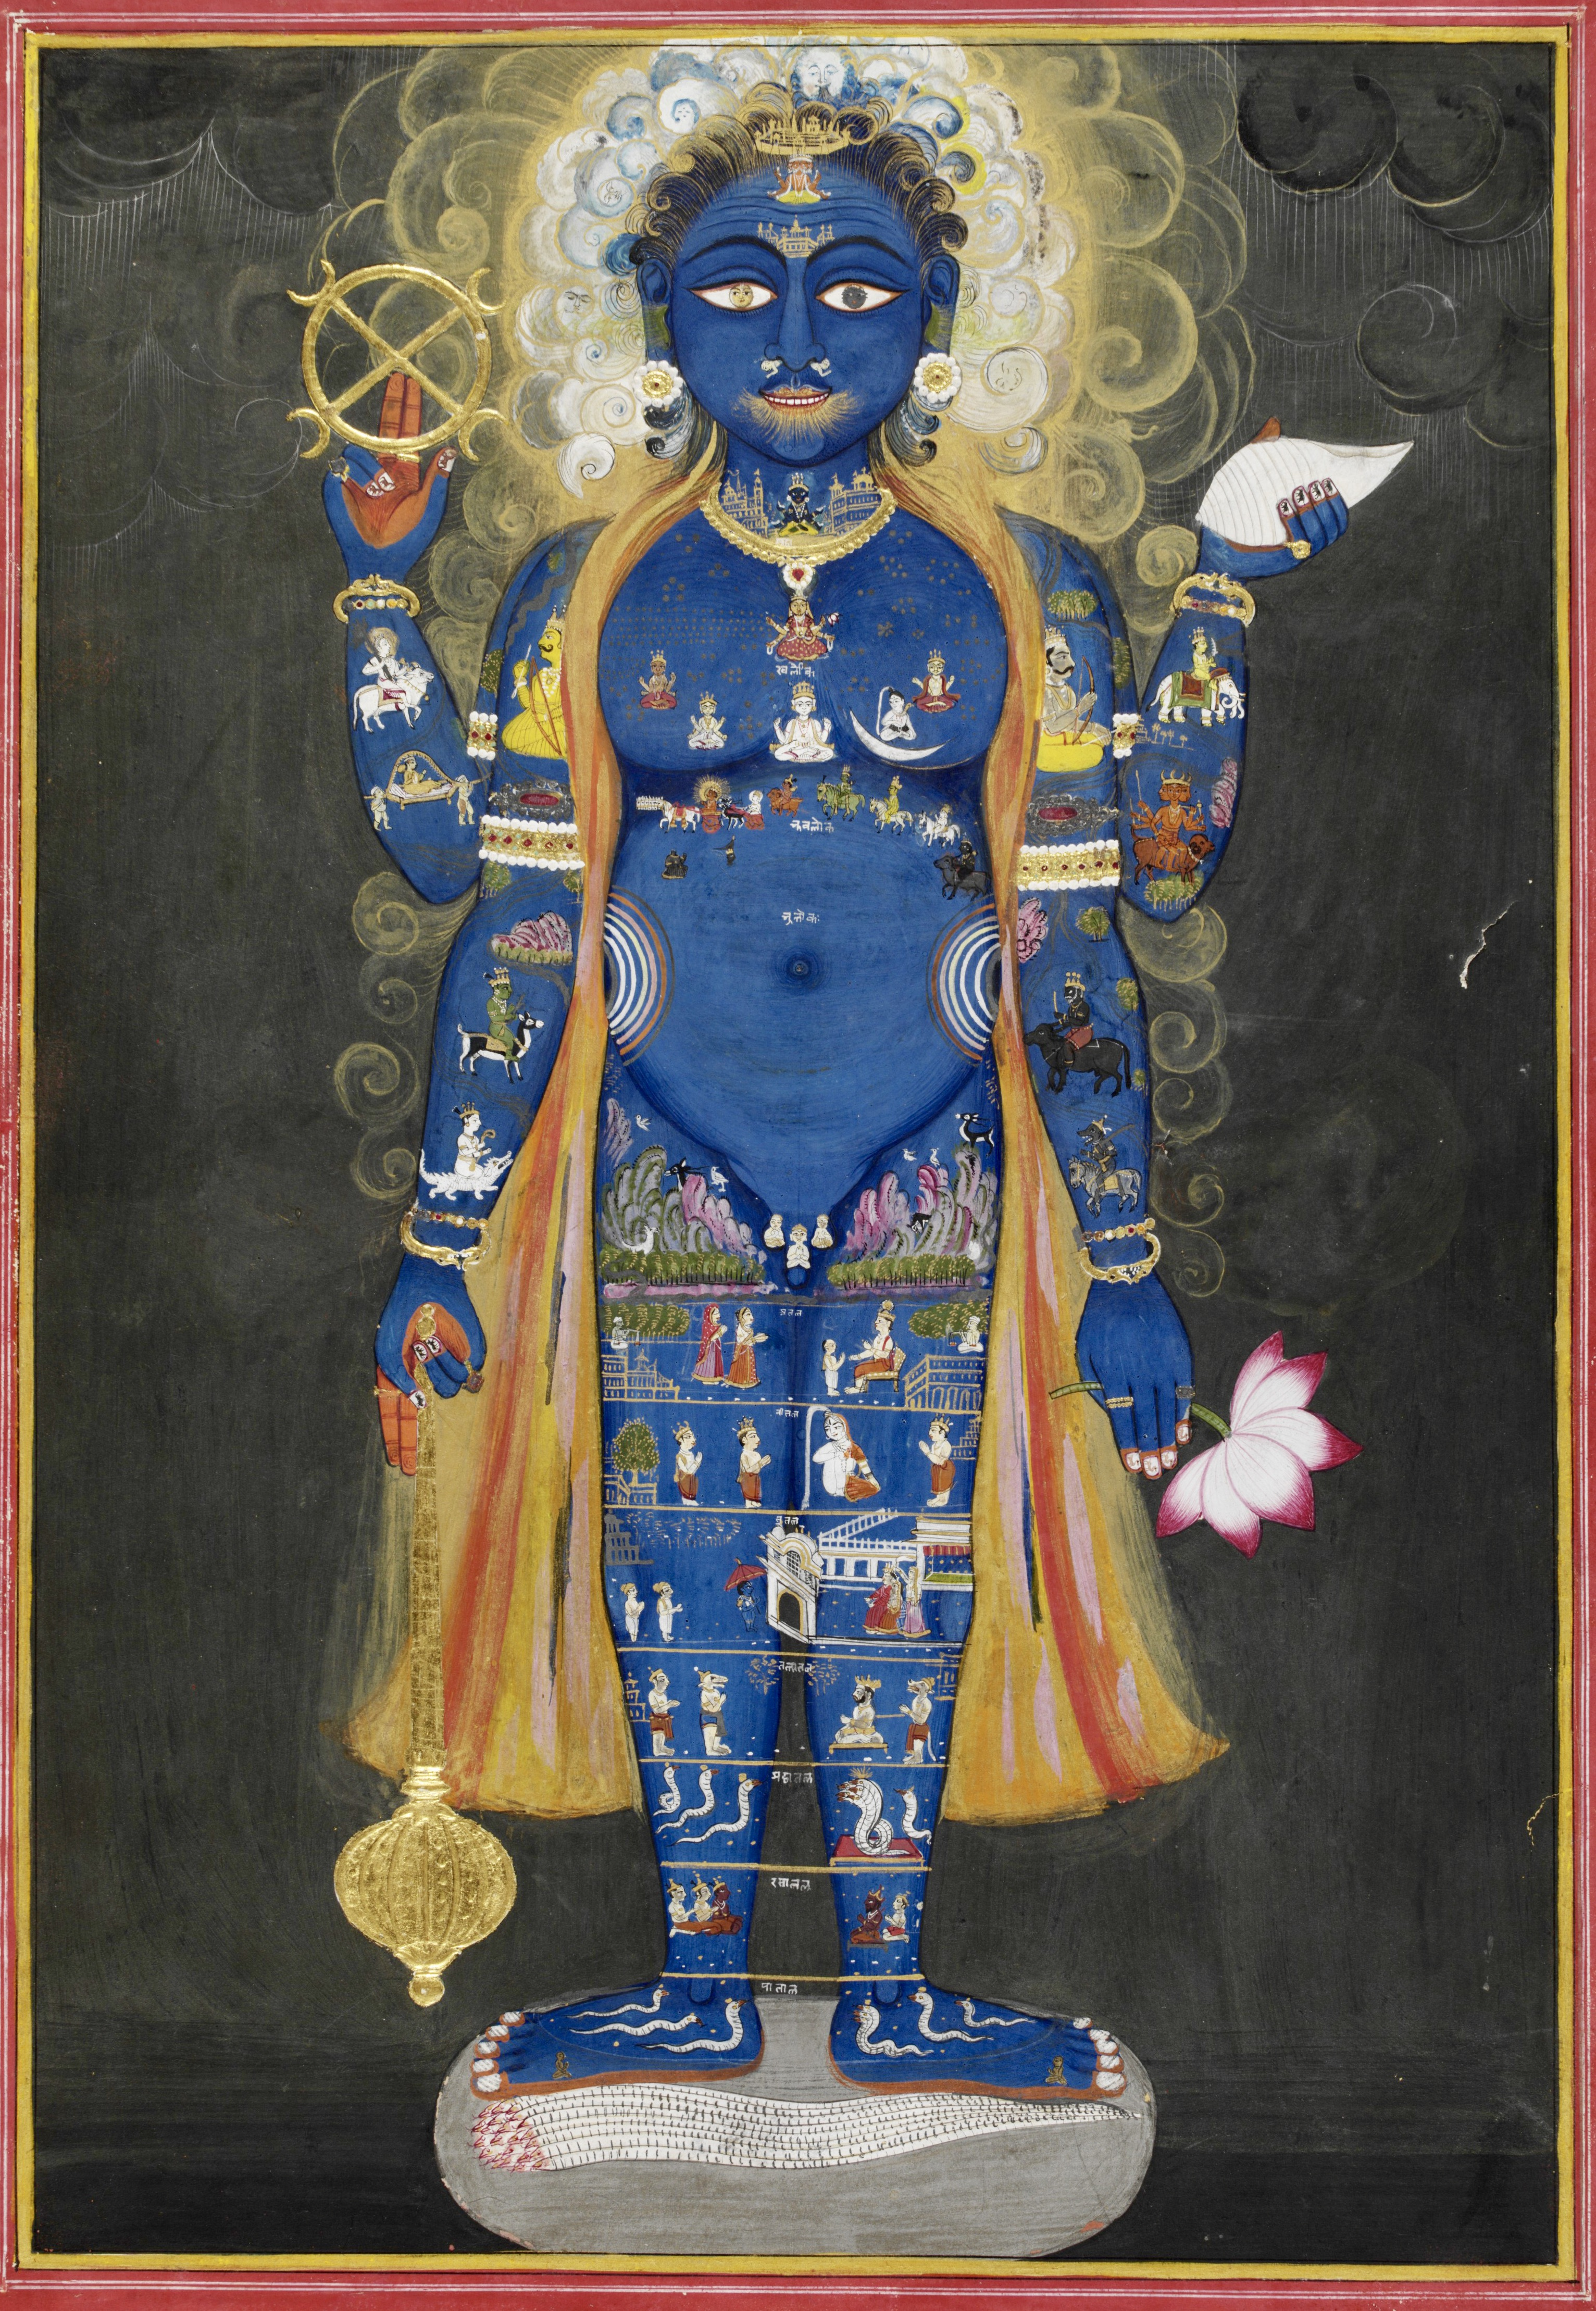
\includegraphics[width=1\textwidth]{pics/Vishnu_Vishvarupa_cropped.jpg}
	\caption{Viṣṇu Viśvarūpa, India, Rajasthan, Jaipur, ca. 1800–1820, Opaque watercolor and gold on paper, 38.5 × 28 cm, Victoria and Albert Museum, London, Given by Mrs. Gerald Clark.}
	\label{fig1}
      \end{figure}
\clearpage
  \begin{figure}[ht]
	\centering
  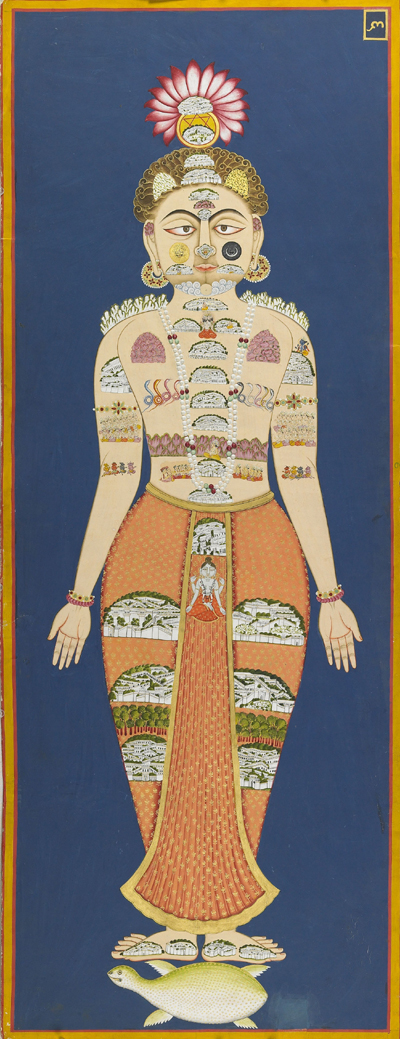
\includegraphics[width=0.5\textwidth]{pics/The_Equivalence_of_Self_and_Universe_(detail),_folio_6_from_the_Siddha_Siddhanta_Paddhati,_(Bulaki),_1824_(Samvat_1881);_122_x_46_cm._Mehrangarh_Museum_Trust..jpg}
	\caption{The Equivalence of Self and Universe (detail), folio 6 from the \textit{Siddhasiddhāntapaddhati} (Bulaki), India, Rajasthan, Jodhpur, 1824 (Samvat 1881), 122 x 46 cm, RJS 2378, Mehragarh Museum Trust.}
	\label{fig2}
      \end{figure}
      % \end{landscape}


\chapter{Bibliography}
 \label{sec:bibli}
   \clearpage
\newpage 
\thispagestyle{empty}
\quad  \addtocounter{page}{-1}

\printbibliography[heading=subbibintoc, title=Consulted Manuscripts, keyword=codex]

\printbibliography[heading=subbibintoc, title=Printed Editions, keyword=printsource]

\printbibliography[heading=subbibintoc, title=Secondary Literature, keyword=seclit]

\printbibliography[heading=subbibintoc, title=Online Sources, keyword=onlinesource]

\end{document}
